\documentclass[11pt]{article}

% "preprint" gives a clean, readable copy with page numbers and no line
% numbers. Switch to "review" for an anonymised submission with line numbers,
% or "final" for the camera-ready.
\usepackage[preprint]{acl}

% Review mode only: send column-1 line numbers to the left margin and column-2
% line numbers to the right margin. The ACL style asks lineno for `switch', but
% lineno only honours that in pagewise mode, which the style does not turn on, so
% by default both columns are numbered on the left. Column 2's numbers then sit
% linenumbersep (45.5pt) to the left of a column whose gutter is only 17pt wide,
% which lands them on top of column-1 text. This is the same \if@firstcolumn test
% lineno itself uses to record the column. Guarded so preprint/final builds,
% where \makeLineNumber does not exist, are unaffected.
\makeatletter
\@ifundefined{makeLineNumber}{}{%
  \renewcommand\makeLineNumber{%
    \if@firstcolumn\makeLineNumberLeft\else\makeLineNumberRight\fi}%
}
\makeatother

\usepackage{times}
\usepackage{latexsym}
\usepackage[T1]{fontenc}
\usepackage[utf8]{inputenc}
\usepackage{microtype}
\usepackage{inconsolata}
\usepackage{graphicx}
\usepackage{booktabs}
\usepackage{balance}
\usepackage{float}
\usepackage{adjustbox}
\usepackage{amsmath}
\usepackage{amssymb}
\usepackage{tikz}
\usetikzlibrary{positioning,arrows.meta,fit,backgrounds,calc,shapes.geometric,shadows,shadows.blur}
\usepackage[edges]{forest}
\usepackage{xcolor}
\usepackage{colortbl}
\usepackage[most]{tcolorbox}
\usepackage{pifont}
\usepackage{fontawesome5}
\hypersetup{
  pdftitle={Can We Believe What Large Language Models Do? A Survey of Validity Threats in Behavioral Studies},
  pdfauthor={Dao Sy Duy Minh, Huynh Trung Kiet, Chi-Nguyen Tran, Nguyen Lam Phu Quy, Phu-Hoa Pham},
  pdfsubject={Validity and reliability of behavioral evaluations of large language models},
  pdfkeywords={large language models, behavioral evaluation, validity, reliability, generalizability, machine psychology, LLM-as-a-judge}
}
\newcommand{\cmark}{\textcolor{tierC}{\ding{51}}}
\newcommand{\xmark}{\textcolor{black!30}{\ding{55}}}
\newcommand{\pmark}{\textcolor{tierB}{$\bullet$}}

% palette (matched to the Figure 1 hero: ink borders + card fills + tier accents)
\definecolor{pipe}{RGB}{28,28,28}
\definecolor{ink}{RGB}{28,28,28}
\definecolor{tierA}{RGB}{55,48,163}    % reliability  (indigo, = hero)
\definecolor{tierB}{RGB}{146,64,14}    % validity     (amber-brown, = hero)
\definecolor{tierC}{RGB}{4,106,56}     % generalizability (green, = hero)
\definecolor{tierAbg}{RGB}{225,231,248}
\definecolor{tierBbg}{RGB}{252,243,207}
\definecolor{tierCbg}{RGB}{215,235,211}

% taxonomy palette: one hue per tier, three lightness steps
\definecolor{txAdark}{RGB}{55,48,163}\definecolor{txAmid}{RGB}{199,205,247}\definecolor{txAlite}{RGB}{237,239,253}
\definecolor{txBdark}{RGB}{146,64,14}\definecolor{txBmid}{RGB}{250,224,175}\definecolor{txBlite}{RGB}{254,246,230}
\definecolor{txCdark}{RGB}{4,106,56}\definecolor{txCmid}{RGB}{190,229,203}\definecolor{txClite}{RGB}{236,250,241}
\definecolor{txroot}{RGB}{51,65,85}\definecolor{txrootbg}{RGB}{226,232,240}
\definecolor{cardblue}{RGB}{216,229,244}
\definecolor{cardcream}{RGB}{252,243,207}
\definecolor{cardpink}{RGB}{246,212,208}
\definecolor{cardgreen}{RGB}{215,235,211}
\definecolor{rootbg}{RGB}{216,229,244}
\definecolor{leafbg}{RGB}{252,250,246}
\definecolor{takebg}{RGB}{255,249,230}
\definecolor{takerule}{RGB}{201,142,20}
\definecolor{taketitle}{RGB}{140,96,10}

% Soft pastel palette for the icon-flow figures (modern, grayscale-safe)
\definecolor{psBlue}{HTML}{DCEBF7}\definecolor{psBlueL}{HTML}{6FA8DC}
\definecolor{psGreen}{HTML}{D9EFDD}\definecolor{psGreenL}{HTML}{6FBF84}
\definecolor{psPurple}{HTML}{E7DEF6}\definecolor{psPurpleL}{HTML}{A88BD6}
\definecolor{psAmber}{HTML}{FCECD2}\definecolor{psAmberL}{HTML}{E1A44C}
\definecolor{psRed}{HTML}{FBDDDA}\definecolor{psRedL}{HTML}{DD8683}
\definecolor{psTeal}{HTML}{D6F0EC}\definecolor{psTealL}{HTML}{5FB6AB}
\definecolor{psInk}{HTML}{27313F}
\definecolor{psGray}{HTML}{EEF1F5}\definecolor{psGrayL}{HTML}{9AA6B2}
\newcommand{\ic}[1]{{\large #1}}

% Colored "Takeaway" callout box with a full-width tinted title bar.
% Usage: \begin{takeaway}{1}{Short title} ... \end{takeaway}
\newtcolorbox{takeaway}[2]{
  enhanced, breakable, boxrule=1pt, arc=3pt,
  colback=takebg, colframe=takerule,
  coltitle=taketitle, colbacktitle=takerule!20,
  fonttitle=\bfseries\small,
  title={\faLightbulb[regular]\,\ Takeaway~#1 \,\raisebox{0.2ex}{\scriptsize\textbullet}\,\ #2},
  left=8pt, right=8pt, top=5pt, bottom=6pt,
  lefttitle=8pt, toptitle=3pt, bottomtitle=3pt, righttitle=8pt,
  fontupper=\small, before skip=7pt, after skip=7pt,
}

\title{Can We Believe What Large Language Models Do?\\
A Survey of Validity Threats in Behavioral Studies}

\author{%
  Dao Sy Duy Minh$^{\dagger}$ \quad
  Huynh Trung Kiet$^{\dagger}$ \quad
  Chi-Nguyen Tran \\
  Nguyen Lam Phu Quy \quad Phu-Hoa Pham \\
  Faculty of Information Technology, University of Science, VNU-HCM \\
  $^{\dagger}$Equal contribution
}

\begin{document}
\maketitle

\begin{abstract}
Researchers infer traits, preferences, strategies, and values from
language-model outputs. Yet a model can give a different
answer when wording, option order, scoring, or context changes. Existing surveys
organise this literature by behavioural domain or system type. We
instead organise it around the validity of the inference from a tested response
to a broader claim.

We separate reliability, validity, and generalizability, then synthesise six
threats: prompt and format
sensitivity, order bias, construct mismatch, scoring-target mismatch,
population misrepresentation, and failure to transfer beyond the tested setting.
We trace these threats across machine psychology, game-theoretic evaluation,
social simulation, and language-model-as-a-judge.

We turn the taxonomy into an audit checklist and a claim-relative diagnostic,
the \emph{fragility fraction}, which measures how much observed variation is
associated with a declared change to the test. Public-data re-analyses show why
scope matters: a difficulty-matched comparison assigns a larger strict fraction
to MoralChoice than to MMLU, but the multiplier changes with the template draw
and item filter. It is not a property of either task family. Likewise, a
$94$-point preference movement is a single-setting extreme, not a typical
effect. The central lesson is to report what the tested measurement supports,
not what one output appears to reveal.
\end{abstract}

\begin{figure}[t!]
\centering
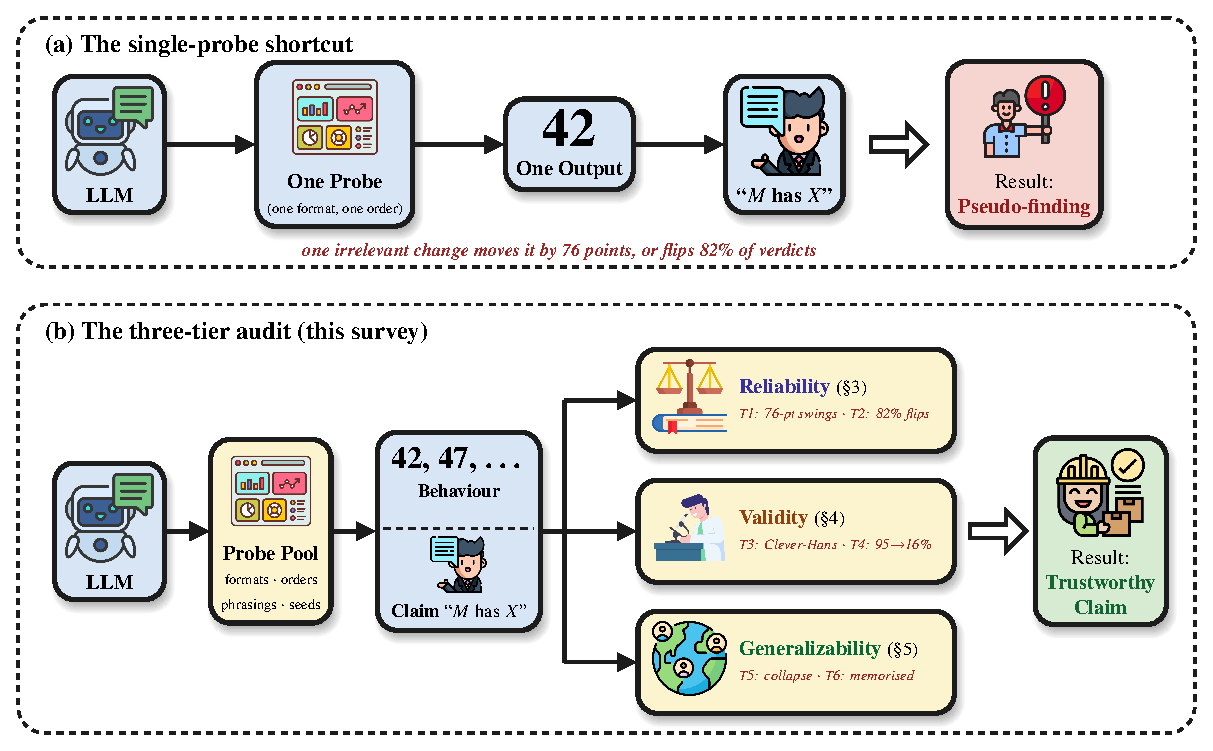
\includegraphics[width=\columnwidth]{figures/core/tikz_hero.pdf}
\caption{\textbf{Is it the model, or the measurement?}
\textbf{(a)}~A single probe promotes one score directly to an unqualified trait
claim. In documented extreme settings, format changes move accuracy by up to
$76$ points \cite{sclar2024quantifying}, and answer order flips $82.5\%$ of one
judge comparison \cite{wang2024fair}. \textbf{(b)}~The audit measures probe
variation, tests the construct and scoring rule, and checks transfer before
stating a claim with its scope.}
\label{fig:hero}
\end{figure}


\section{Introduction}
\label{sec:intro}

Psychology spent much of the last century learning a hard lesson: before you
can claim that a test score reveals an underlying trait, you must show that
the measurement is trustworthy. That discipline has a name, measurement
theory, and it rests on three questions. Is the measurement stable when you
change things that should not matter (reliability)? Does it measure the
thing you claim it measures (validity)? And does what you found on the test
carry over to the population or situation you care about (generalizability)?
Seventy years of psychometrics turned these questions into standard practice
\cite{cronbach1955construct,messick1995validity}.

The rise of large language models has produced a literature that needs this
discipline but does not yet apply it consistently, treating models as agents and
experimental subjects \cite{rahwan2019machine,hagendorff2023machine} in four main
forms: strategic and economic games where models play each other or people
\cite{akata2025playing,fontana2025nicer,bianchi2024negotiation}; \emph{silicon
sampling}, where a model is given a persona so it can stand in for a survey
respondent or a whole society
\cite{argyle2023out,santurkar2023whose,park2023generative}; machine psychology,
which hands models the questionnaires built to measure human personality, values
and cognitive biases
\cite{binz2023cognitive,echterhoff2024cognitive,ye2025psychometrics}; and the
language-model-as-a-judge setting, which reads comparative verdicts as stable
preferences \cite{zhengmt2023judging,gu2024judge}.

A recurring move reduces outputs, including game moves, ratings, survey
answers, and comparative verdicts, to one score. It then treats that score as
evidence that the model has a stable characteristic. We call this a
\emph{stable-trait claim}: the response is taken to reveal a trait, preference,
or strategy that should persist beyond the exact prompt.

Existing surveys provide useful maps organised around other questions. Some
group studies by what is measured, such as personality or values
\cite{hagendorff2023machine,ye2025psychometrics}. Others group them by system
design, such as single-agent versus multi-agent systems
\cite{xi2023rise,wanglei2024autonomous}; by whether the interaction concerns an
individual, a group, or a society \cite{mou2024individual}; by game family
\cite{sun2025gametheory}; or by evaluation application, such as judging model
answers, evaluating agents, or simulating personas
\cite{gu2024judge,yehudai2025evaluation,tseng2024persona}. Validity-oriented work
addresses parts of the problem, but cross-domain surveys do not organise their
evidence around the question that decides what a behavioural score can support:
\textbf{the model produced
this output, but does that entitle us to say it \emph{has} the trait we are
reading into it?} The field names fragments of the problem, prompt sensitivity
here, contamination there, persona instability elsewhere, but treats them as
scattered limitations rather than as the object of study.

This paper makes that inference the main question. The stakes are visible in
Figure~\ref{fig:hero}: individual stress tests report movements of $40$ to $80$
percentage points after changing a prompt format, answer order, or framing while
holding the intended task fixed. These are extreme settings, but the movement
can exceed the effect a study set out to interpret.

In three documented cases the headline interpretation changes or weakens under
a specified intervention: apparent theory of mind, measured
cooperation between a model and its reasoning-tuned variant, and the opinion
distribution of a simulated population (Appendix~\ref{app:catalogue}). These are
worst-case existence proofs from settings chosen to expose a threat, not
estimates of how often it bites, and we tag every magnitude with its setting.

We import the reliability, validity, and generalizability framework of
measurement theory and reorganise the field into a taxonomy of six recurring
threats (Figure~\ref{fig:taxonomy}). Adjacent surveys and validity frameworks
already cover important pieces \cite{lin2025prompts,wallach2025position,%
bean2025measuring,ivanova2025evaluate}; our narrower novelty claim is their
cross-domain synthesis: strategic games, social simulation, machine psychology,
and judging under one measurement-threat taxonomy, organised by whether the
evidence supports the conclusion rather than by the topic being studied
(Section~\ref{sec:related}).

Section~\ref{sec:frame} lays out the steps from a tested response to a
stable-trait claim and locates the three tiers along them;
Sections~\ref{sec:reliability} to~\ref{sec:general} review the six threats
tier by tier; Section~\ref{sec:mmul} shows that they also recur beyond
forced-choice English text; Section~\ref{sec:checklist} turns them into a validity
checklist; and Section~\ref{sec:related} positions the survey against prior
work.

\section{The Behavioural-Inference Pipeline}
\label{sec:frame}

\begin{figure}[t]
\centering
\resizebox{\columnwidth}{!}{%
\begin{tikzpicture}[
  font=\small, node distance=0pt,
  stage/.style={draw=ink, line width=1.6pt, rounded corners=8pt, fill=#1,
                text=ink, align=center, inner sep=5pt,
                minimum height=1.9cm, minimum width=2.15cm,
                blur shadow={shadow blur steps=8, shadow xshift=1.4pt,
                shadow yshift=-2.6pt, shadow blur radius=2.6pt,
                shadow opacity=32}},
  flow/.style={-{Triangle[length=3mm,width=2.8mm]}, line width=1.5pt, ink},
  pill/.style={rounded corners=6pt, fill=#1, draw=#1, text=white,
               font=\scriptsize\bfseries, inner xsep=6pt, inner ysep=3pt},
]
\node[stage=cardcream] (probe)
  {
\includegraphics[width=0.95cm]{figures/icons/paper/satisfaction.png}\\[2pt]\textbf{Probe /}\\\textbf{elicitation}};
\node[stage=cardblue, right=1.85cm of probe] (obs)
  {
\includegraphics[width=0.95cm]{figures/icons/paper/observation.png}\\[2pt]\textbf{Observed}\\\textbf{behaviour}};
\node[stage=cardblue, right=1.85cm of obs] (claim)
  {
\includegraphics[width=0.95cm]{figures/icons/paper/scientist.png}\\[2pt]\textbf{Claim:}\\\textbf{``$M$ has $X$''}};
\node[stage=cardgreen, right=1.85cm of claim] (dep)
  {
\includegraphics[width=0.95cm]{figures/icons/paper/startup.png}\\[2pt]\textbf{Deployment /}\\\textbf{population}};

\draw[flow] (probe) -- (obs);
\draw[flow] (obs) -- (claim);
\draw[flow] (claim) -- (dep);

\node[pill=tierA] at ($(probe)!0.5!(obs)+(0,1.22)$)  {T1\,\,T2};
\node[pill=tierB] at ($(obs)!0.5!(claim)+(0,1.22)$)  {T3\,\,T4};
\node[pill=tierC] at ($(claim)!0.5!(dep)+(0,1.22)$)  {T5\,\,T6};
\node[font=\scriptsize\bfseries, text=tierA] at ($(probe)!0.5!(obs)+(0,0.82)$)  {Reliability};
\node[font=\scriptsize\bfseries, text=tierB] at ($(obs)!0.5!(claim)+(0,0.82)$)  {Validity};
\node[font=\scriptsize\bfseries, text=tierC] at ($(claim)!0.5!(dep)+(0,0.82)$)  {Generaliz.};
\end{tikzpicture}}
\caption{The behavioural-inference pipeline and where each tier attacks it. A
study elicits a behaviour with a \emph{probe}, observes it, reads off a
\emph{claim} that model $M$ has construct $X$, and generalises to a
\emph{deployment}. Reliability threats corrupt the measurement, validity threats
break the link to the named construct, and generalizability threats break the
link to the population the claim is about.}
\label{fig:pipeline}
\end{figure}

\begin{figure*}[t]
\centering
\adjustbox{max width=\textwidth,max totalheight=0.34\textheight}{%
\begin{forest}
  forked edges,
  for tree={
    grow'=east,
    draw,
    rounded corners=2pt,
    align=left,
    font=\tiny,
    edge={semithick,txroot!60},
    l sep=4mm,
    s sep=0.35mm,
    inner sep=1.6pt,
    anchor=west,
    child anchor=west,
  },
  [{Validity Threats to\\Behavioural Claims},fill=txrootbg,draw=txroot,line width=1pt,text=txroot,font=\scriptsize\bfseries,
   rotate=90,anchor=north,align=center
    %% ==== TIER 1 ====
    [{Tier 1\\Reliability\\\S\ref{sec:reliability}},fill=txAmid,draw=txAdark,line width=1pt,text=txAdark,
     font=\tiny\bfseries,align=center
      [{T1 Prompt \&\\Format Sensitivity\\\S\ref{sec:t1}},fill=txAmid,draw=txAdark,line width=0.7pt,font=\tiny\bfseries
        [{\textbf{Format}: FormatSpread \citep{sclar2024quantifying}, delimiters \citep{su2025singlechar}, DOVE \citep{habba2025dove}, structure \citep{tam2024format}, \citep{lu2022fantastically,salinas2024butterfly,zhao2021calibrate}},fill=txAlite]
        [{\textbf{Paraphrase}: \citep{mizrahi2024state}, ParaRel \citep{elazar2021measuring}, \citep{binz2023cognitive,pecher2026underspec,zhou2024paraphrase,jang2023consistency,raj2025chainguidance}},fill=txAlite]
        [{\textbf{Run-to-run}: \citep{atil2025nondeterminism}, greedy \citep{song2024greedy}, numerical \citep{yuan2025numerical}, code \citep{ouyang2025chatgptnondet}, seeds \citep{bui2025seeds,hochlehnert2025sober,fu2026tokenprob}},fill=txAlite]
        [{\textbf{Sensitivity indices}: POSIX \citep{chatterjee2024posix}, $\Pi_m$ \citep{romanou2026brittlebench}, artefact? \citep{hua2025flaw}, worst \citep{cao2024worst}, \citep{zhu2024promptrobust,lior2025reliableeval,zhuo2024prosa}},fill=txAlite]
      ]
      [{T2 Order \&\\Presentation Bias\\\S\ref{sec:t2}},fill=txAmid,draw=txAdark,line width=0.7pt,font=\tiny\bfseries
        [{\textbf{Forced choice}: \citep{zheng2024selectors,pezeshkpour2024large}, MCSB \citep{robinson2023mcsb}, \citep{wei2024unveiling}, choices-only \citep{balepur2024artifacts}, surveys \citep{dominguez2024questioning}},fill=txAlite]
        [{\textbf{Judge}: FairEval \citep{wang2024fair}, \citep{shi2025judging}, MT-Bench \citep{zhengmt2023judging}, CALM \citep{ye2024justice}},fill=txAlite]
        [{\textbf{Serial position}: \citep{guo2024serial}, premise \citep{chen2024premise}, anchoring \citep{huang2025anchoring}, lost-in-middle \citep{liu2024lostmiddle}, primacy \citep{wang2023primacy}, \citep{peysakhovich2023attention}},fill=txAlite]
        [{\textbf{Listwise ranking}: permutation \citep{tang2024permutation}, RankGPT \citep{sun2023rankgpt}, pairwise \citep{qin2024pairwise}, setwise \citep{zhuang2024setwise}, self-calib \citep{ren2024selfcalibrated}},fill=txAlite]
        [{\textbf{Debiasing}: CalibraEval \citep{li2025calibraeval}, batch \citep{zhou2024batchcal}, label bias \citep{reif2024labelbias}, node-prune \citep{choi2025nodepruning}, order-free \citep{mcilroyyoung2024setbased}},fill=txAlite]
      ]
    ]
    %% ==== TIER 2 ====
    [{Tier 2\\Validity\\\S\ref{sec:validity}},fill=txBmid,draw=txBdark,line width=1pt,text=txBdark,
     font=\tiny\bfseries,align=center
      [{T3 Construct\\Validity \S\ref{sec:t3}},fill=txBmid,draw=txBdark,line width=0.7pt,font=\tiny\bfseries
        [{\textbf{Instruments}: \citep{gupta2024self,shu2024dont,serapiogarcia2023personality,petrov2024limited}, psychometrics \citep{li2024psychometrics}, content-val \citep{milano2025content}},fill=txBlite]
        [{\textbf{Structure fails}: \citep{suhr2023challenging,rottger2024political}, IRT \citep{rodriguez2021irt,zhou2025lost,chen2025compact}, factor \citep{wang2025emulate}},fill=txBlite]
        [{\textbf{Response styles}: desirability \citep{salecha2024social}, acquiescence \citep{braun2025acquiescence}, forced choice \citep{okada2026desirability}},fill=txBlite]
        [{\textbf{Stated vs enacted}: \citep{han2025illusion,contreras2026native,nunes2024hypocrites}, know-not-do \citep{huang2026knowing}, \citep{taubenfeld2026dispositions,ai2024selfknowledge}},fill=txBlite]
        [{\textbf{Invariance}: \citep{zierahn2026without}, DIF \citep{zeinfeld2026dif}, PATCH \citep{fang2024patch}, temporal \citep{bodroza2024temporal}, \citep{bhandari2025evaluating,ma2026stable}},fill=txBlite]
        [{\textbf{Shortcuts}: \citep{ullman2023trivial}, \citep{shapira2024clever}, \citep{guo2023suspicion}},fill=txBlite]
        [{\textbf{Artefacts}: \citep{schaeffer2023mirage}, \citep{hufrank2024auxiliary}, \citep{meyer2026apparent}, \citep{walsh2026convenient}},fill=txBlite]
      ]
      [{T4 Normative-\\Benchmark \S\ref{sec:t4}},fill=txBmid,draw=txBdark,line width=0.7pt,font=\tiny\bfseries
        [{\textbf{Rationality}: \citep{akata2025playing}, GTBench \citep{duan2024gtbench}, $\gamma$-bench \citep{huang2025gama}, \citep{fan2024rational}, QRE \citep{pechon2026qre}},fill=txBlite]
        [{\textbf{Choice axioms}: \citep{chen2023emergence}, GARP \citep{wen2025garp}, \citep{seror2024moralmind,tak2026sparks}, prospect \citep{jia2024decision}},fill=txBlite]
        [{\textbf{Stated vs revealed}: \citep{gu2025revealed}, elicitation \citep{mahajan2026mindgap}, incentives \citep{zhou2026incentives}, \citep{yamin2026revealed}, tactics \citep{wang2025expecon}},fill=txBlite]
        [{\textbf{Framing}: \citep{lore2024strategic,gandhi2023strategic,zhang2024klevel}, context \citep{robinson2025framing}, cross-family \citep{wang2026framing}},fill=txBlite]
        [{\textbf{Human-likeness}: \citep{fontana2025nicer}, \citep{li2025spontaneous}, \citep{mei2024behavioral}},fill=txBlite]
        [{\textbf{Strategic depth}: level-$k$ \citep{teo2026levelk}, CHBench \citep{liu2025chbench}, \citep{kader2024emergence,jia2025agentic}, theory \citep{liu2024levelk}},fill=txBlite]
      ]
    ]
    %% ==== TIER 3 ====
    [{Tier 3\\Generalizability\\\S\ref{sec:general}},fill=txCmid,draw=txCdark,line width=1pt,text=txCdark,
     font=\tiny\bfseries,align=center
      [{T5 Population \&\\Aggregation \S\ref{sec:t5}},fill=txCmid,draw=txCdark,line width=0.7pt,font=\tiny\bfseries
        [{\textbf{Silicon sampling}: \citep{argyle2023out,horton2023homo,aher2023turing}, causal \citep{gui2023causal}, self-reports \citep{park2024selfreports}, debate \citep{dillion2023replace,harding2024cannot}},fill=txClite]
        [{\textbf{Aggregation}: OpinionQA \citep{santurkar2023whose}, GlobalOpinionQA \citep{durmus2023global}, PRISM \citep{kirk2024prism}, \citep{alkhamissi2024investigating,hucollier2024persona,beck2024sensitivity,feng2023pretraining}},fill=txClite]
        [{\textbf{Flatten / skew}: \citep{atari2023which,wang2025misportray,li2025silicon}, caricature \citep{cheng2023compost}, CAMeL \citep{naous2024beer}, \citep{cui2024replace,bisbee2024synthetic}},fill=txClite]
        [{\textbf{Calibration}: \citep{li2026spirit}, PPI \citep{angelopoulos2023ppi,angelopoulos2023ppiplus}, cross-PPI \citep{zrnic2024crossppi}, DSL \citep{egami2023dsl}, limit \citep{dorner2025limits}, \citep{gligoric2025confident}},fill=txClite]
      ]
      [{T6 Ecological\\\& Leakage \S\ref{sec:t6}},fill=txCmid,draw=txCdark,line width=0.7pt,font=\tiny\bfseries
        [{\textbf{Transfer}: iAgents \citep{liu2024autonomous}, GovSim \citep{piatti2024govsim}, CoopEval \citep{tewolde2026coopeval}, \citep{liu2025machines}},fill=txClite]
        [{\textbf{Contamination}: \citep{sainz2023nlp}, \citep{oren2024proving}, ConStat \citep{dekoninck2024constat}, \citep{duan2024mimir}, \citep{shi2024mink}},fill=txClite]
        [{\textbf{Eval awareness}: \citep{vanderweij2025sandbagging}, \citep{needham2025evalaware}, SAD \citep{laine2024sad}, \citep{berglund2023outofcontext}, \citep{jung2025psychometric}},fill=txClite]
        [{\textbf{User pressure}: sycophancy \citep{sharma2024sycophancy}, rebuttal \citep{kim2025rebuttal}, synth-fix \citep{wei2023sycophancy}, persuasion \citep{xu2024earthflat}, \citep{perez2023modeleval}},fill=txClite]
        [{\textbf{Emergence}: \citep{park2023generative}, \citep{ashery2025emergent}, CRSEC \citep{ren2024emergence}, \citep{hua2024waragent}, \citep{chuang2024simulating}},fill=txClite]
        [{\textbf{Rich games}: Werewolf \citep{xu2023werewolf}, AvalonBench \citep{light2023avalonbench}, \citep{bianchi2024negotiation,fish2024collusion}, Diplomacy \citep{mukobi2023welfare}},fill=txClite]
        [{\textbf{Interaction}: SOTOPIA \citep{zhou2024sotopia}, lifelong \citep{goel2025lifelong}, clembench \citep{chalamalasetti2023clembench}, \citep{abdulhai2023lmrlgym}, MINT \citep{wang2024mint}, $\tau$-bench \citep{yao2024taubench}},fill=txClite]
        [{\textbf{Composition gap}: \citep{fu2026moreagents,tang2025taskcomplexity}, failures \citep{cemri2025mast}, scaling \citep{chen2024llmcalls}, debate \citep{du2023debate}, \citep{zhang2024collab}},fill=txClite]
        [{\textbf{Misconduct}: collusion \citep{agrawal2025collusion,tian2026promptcollusion}, stego \citep{motwani2024collusion}, privacy \citep{mireshghallah2024confaide}, \citep{abdelnabi2023negotiation}, attacks \citep{tian2023evilgeniuses}},fill=txClite]
      ]
    ]
  ]
\end{forest}}
\caption{Full taxonomy of the six validity threats, with representative
citations, organised by the three tiers of measurement theory. Each tier maps
to one section (\S\ref{sec:reliability}, \S\ref{sec:validity},
\S\ref{sec:general}); each leaf groups the studies surveyed for that threat.}
\label{fig:taxonomy}
\end{figure*}

Many studies here make the same three-step move, so it is worth walking through
it once, concretely, before auditing it.

\textbf{Ask.} The study writes a \emph{probe}, meaning the input it puts in front
of the model, written $c$: a survey question, a game, or two answers to rank. Say
it is ``Would you rather keep a promise or prevent a small harm?'', options in
that order.

\textbf{Record.} The model answers, and answers differently if asked again,
because generation is sampled. So what comes back is not one answer but a spread
of answers with probabilities, written $\pi_M(\cdot\mid c)$ and read as ``how
model $M$ tends to respond to $c$''. The study reduces that spread to one number,
usually how often the first option is chosen, averaged over many probes.

\textbf{Conclude.} From that number the study says the model \emph{has}
something: a trait, preference, strategy, value, or bias. That something is the
\emph{construct}, written $X$, and it is what the study is really claiming to
measure. When a paper treats $X$ as a stable property that should appear beyond
the tested prompt, we call this a \emph{stable-trait claim}. Such a claim often
also implies that $X$ predicts how the model behaves with real users.

This survey lives in the gap between the last two steps. Recording produces a
number; concluding treats it as evidence about $X$. Everything below asks when
that is allowed.

Psychology separates three questions about a move like this
(Figure~\ref{fig:pipeline}). They are a useful audit order, not a gatekeeping
sequence: evidence about deployment can expose a problem in a supposedly stable
measure. \emph{Reliability} asks whether the number holds still under changes
that should not matter, such as swapping the option order or rewording the
question. \emph{Validity} asks whether a number, stable or not, is measuring
$X$ at all. This requires both an instrument that
still means what it meant when designed for people and an appropriate scoring
standard \cite{cronbach1955construct}. A scoring standard is the rule used to
decide what counts as success. For example, a game choice may be scored against
equilibrium play, while a model judge may be scored against human labels.

Repeatability alone is not enough. \citet{norman2026reliability} evaluated $21$
judge models under several protocols, producing about $541{,}000$ judgments.
Two production-deployed judges had test-retest reliability above $0.95$ while
also showing position bias above $0.10$. In other words, they were highly
consistent when the same input was repeated, but an irrelevant feature, answer
position, still affected the verdict. Earlier controlled order swaps show how
large that problem can become: one ChatGPT comparison returned conflicting
verdicts on $82.5\%$ of examples after the two answers exchanged positions
\cite{wang2024fair}. A judge can therefore be repeatable and still rely on the
wrong cue. \emph{Generalizability} asks whether a valid claim
still holds where it is meant to apply, over the population it represents or the
deployment it predicts. Each question, put to language models, turns up a pair of
recurring threats (Figure~\ref{fig:taxonomy}), and we take them in turn.

\paragraph{Scope and method.} We cover empirical studies that infer a
stable trait from an observed behaviour: strategic and economic games,
multi-agent and cultural simulation, psychometric and cognitive-bias testing,
and judge evaluation where verdicts are read as preferences. The behaviour may
be a forced choice or an open-ended generation; the threats apply to both, and
\S\ref{sec:mmul} shows that the same threat classes recur there. We
privilege studies that manipulate a threat \emph{directly}, varying a probe
detail and reporting how the behaviour moves, since a single number under a
single probe can illustrate a claim but cannot test it.
Appendix~\ref{app:protocol} gives the full protocol, including exclusions, and
Appendix~\ref{app:catalogue} tags every cited magnitude by scope, separating
single-setting extremes from broad results, mechanisms, and mitigations.


\section{Tier 1: Reliability}
\label{sec:reliability}

Reliability asks whether a measured behaviour survives changes that should not
matter: the prompt's format (T1), the order of options or candidates (T2), or
nothing but the random seed. Documented cases fail each test. A single-probe
design therefore cannot tell model variation from probe variation. We
place T2's presentation prior here rather than under validity because, though
systematic, it corrupts the measurement before any construct question arises
(Figure~\ref{fig:pipeline}).

\subsection{Prompt and Format Sensitivity (T1)}
\label{sec:t1}

\textbf{Formats that mean the same thing make one model behave like different
models.}
\citet{sclar2024quantifying} show that meaning-preserving formatting choices,
namely the separators, casing, and spacing of a prompt, produce accuracy
differences of up to $76$ points on a single model (LLaMA-2-13B), and they
propose the FormatSpread procedure so that studies report the spread rather
than one lucky point. \citet{lu2022fantastically} find that simply reordering
the same in-context examples moves performance across the entire range from
near state-of-the-art to near chance. At the scale of whole leaderboards,
\citet{mizrahi2024state} evaluate $20$ models over $6.5$ million instances
and show that the \emph{ranking} of models changes when the instructions are
paraphrased, concluding that single-prompt evaluation is not reproducible and
that studies should report results over many prompts.

\subsection{Order and Presentation Bias (T2)}
\label{sec:t2}

\textbf{Option order is a directional prior, not noise.}
\citet{zheng2024selectors} identify a token-level \emph{selection bias}, an a
priori preference for particular option identifiers such as the letter ``A''.
Moving the correct answer between fixed positions swings multiple-choice
accuracy by up to $17$ points. The paper measures label bias as the standard
deviation of recall across A, B, C, and D. In one zero-shot GPT-3.5 MMLU test,
it is $5.5$. Removing the letters lowers it to $1.0$; randomly permuting them
only lowers it to $5.1$. Thus, shuffling exposes the model's preference for
particular label tokens but does not remove it.

\textbf{Debiasing can dissolve the phenomenon.} Most striking for stable-trait
claims, \citet{dominguez2024questioning} show that survey responses carry a
systematic bias toward the option labelled ``A'', and that once the order is
randomised to remove it, models of every size drift toward the uniform-random
distribution: the apparent ``opinion'' was largely an artefact of presentation. The label prior itself is not one paper's finding, having been
documented independently as a token-level preference and as a separable order
effect \cite{zheng2024selectors,pezeshkpour2024large,wei2024unveiling}.

\begin{takeaway}{1}{Stability must be tested}
Repeating one prompt tests sampling noise, not measurement stability. A claim
about a model should also survive changes that preserve the question, such as
rewording and option order. The largest effects above are warning cases, not
typical values, but independent studies show that the mechanisms recur.
\emph{Fix:} use a fixed, balanced pool of prompts, formats, and orders; report
the full spread and the share of variation caused by those changes.
\end{takeaway}

\section{Tier 2: Validity}
\label{sec:validity}

Even a reliable measurement may not measure the construct it names. Its scoring
standard may also decide the verdict before the model is evaluated. These are
two separable failures, and it helps to keep them apart. Construct validity
(T3) concerns the \emph{instrument}: does the questionnaire, game, or task
elicit the trait it is supposed to elicit, or does the model pass it by a
shortcut? Normative-benchmark validity (T4) concerns the \emph{scoring rule}
applied afterwards: granting that the behaviour was elicited faithfully, is
the standard we score it against, such as rational play or human-likeness,
the right one? A personality questionnaire that a model answers by echoing the
prompt's wording is a T3 failure; a faithfully elicited game choice that we
wrongly call ``irrational'' because we picked the wrong equilibrium concept is
a T4 failure.

\subsection{Construct Validity (T3)}
\label{sec:t3}

\textbf{Human instruments do not automatically keep their meaning on models.} Self-report
personality tests return statistically different trait scores under three prompts
that mean the same thing, so ``the model's Big Five profile'' is not well defined
\cite{gupta2024self}. The instability is systematic: across $17$ models and $693$
items from $39$ psychometric instruments, changing nothing but a prompt's final
punctuation drops the mean valid-response rate from $0.89$ to $0.65$
\cite{shu2024dont}. Whether these instruments transfer at all depends on the
configuration, with one study finding support only for larger instruction-tuned models under structured
administration \cite{serapiogarcia2023personality} and collapsing once the
persona is a specific person's demographic profile, the silicon sampling case
\cite{petrov2024limited}. Assigned traits are \emph{expressed}
\cite{jiang2024personallm} without being stably \emph{measured}, and
forced-choice value inventories such as the Political Compass tell the same
story, recording the constrained format rather than a stable opinion
\cite{rottger2024political}.

Models also carry response styles of their own, a pull toward socially
approved answers and a fixed answer preference that runs opposite to the
human direction, which the instrument records as if it were the trait
\cite{salecha2024social,braun2025acquiescence} (Appendix~\ref{app:tierevidence3}).

Order bias and response style can co-occur. We place a label or position prior
in T2 when the immediate failure is a change under a construct-irrelevant
presentation edit; we place a directional style in T3 when it contaminates the
meaning of a trait score even after presentation is balanced. The distinction is
therefore claim-relative, not a claim that one mechanism can affect only one tier.

\textbf{The construct can be an artefact of the analysis.}
\citet{schaeffer2023mirage} demonstrate that ``emergent abilities'' can appear
under a nonlinear scoring metric and disappear under a linear one, and
\citet{hufrank2024auxiliary} show that measured capability partly
reflects incidental task demands imposed by the researcher's design. The
starkest evidence is a variance decomposition of personality profiles across
$56$ models: between $81$ and $90\%$ of the variation between models is a
directional response bias, a tendency to lean toward one end of the scale
regardless of content, against only $9$ to $16\%$ in humans
\cite{meyer2026apparent}, supported independently by the finding that only $3\%$
of Big Five score variance lies between models across $244$ of them, and by the
response styles documented separately
\cite{zierahn2026without,salecha2024social,braun2025acquiescence}. When the number depends this much on how the
instrument is built, ``the model has $X$'' is a statement about the instrument.
Edits that preserve the intended meaning are a useful first check. A stronger
test examines the response structure: fit an item-response or factor model and
ask whether the items relate to the construct as they do for humans. Such tests
are now applied directly to language models
\cite{rodriguez2021irt,zhou2025lost,wang2025emulate}. A shortcut and a genuine
construct can produce similar averages but different response patterns.

\subsection{Normative-Benchmark and Scoring-Target Validity (T4)}
\label{sec:t4}

\textbf{Models struggle against the rationality benchmark.} Game-theoretic
evaluation usually scores behaviour against equilibrium play, the outcome from
which no player can profitably deviate \cite{nash1950equilibrium}. Models excel
in the defection-friendly iterated Prisoner's Dilemma yet perform poorly on
simple coordination games \cite{akata2025playing}, and dedicated suites confirm
broad strategic-reasoning limits, with even GPT-4 diverging from both human
behaviour and rational play
\cite{duan2024gtbench,huang2025gama,fan2024rational,light2023avalonbench}.
Extra reasoning support moves that behaviour substantially, whether by showing beliefs
explicitly \cite{gandhi2023strategic} or by prompting recursive depth of
reasoning \cite{zhang2024klevel}, so measured ``strategic depth'' is partly a
property of the elicitation rather than of the model.

\textbf{The benchmark itself is fragile.} \citet{lore2024strategic}
separate a game's structure from its contextual framing and find that both can
substantially change behaviour, with their relative importance differing by
model \cite{tversky1981framing,robinson2025framing}, so a single scenario
cannot separate a strategic disposition from a surface response. Deviation from
equilibrium is moreover ambiguous between irrationality and optimising a
different objective. We can separate them by working backward from the choices
to infer the objective they fit, then asking whether the choices are consistent
under that objective.

Payoff magnitude and prompt language can also change the inferred strategy
\cite{huynh2026payoff}; Appendix~\ref{app:t4evidence} gives the comparison.

\textbf{Different scoring standards answer different questions.} Scored against
equilibrium play, models look weakly strategic
\cite{akata2025playing,duan2024gtbench}. Scored against the axioms of consistent
choice, models can look \emph{more} consistent than human subjects, with
budget choices satisfying utility maximisation at above-human rates and most
major models acting as if maximising a stable utility function on moral dilemmas
\cite{chen2023emergence,seror2024moralmind,tak2026sparks}. These papers do not
re-score one identical output set, so they do not isolate the scoring standard as a
causal factor. They do show that ``strategic'' and ``coherent'' are different
claims: equilibrium play requires modelling another player, while choice
consistency does not. Reporting the scoring rule therefore fixes the meaning of
the result. Strategic depth needs the same care
\cite{wen2025garp,gu2025revealed,mahajan2026mindgap,teo2026levelk,liu2025chbench}.

\begin{takeaway}{2}{A score is not yet a construct}
A stable score describes performance on a test. It does not by itself show that
the model has the named trait or strategy. This gap persists across domains
\cite{ye2025psychometrics,lin2025prompts,lin2026validity}. \emph{Fix:} test
whether meaning-preserving changes keep the interpretation stable, compare
alternative measures, and state the scoring target. In particular, separate
``incoherent'' from ``consistent under a different objective''.
\end{takeaway}

\section{Tier 3: Generalizability}
\label{sec:general}

Stable-trait claims usually reach beyond the test, either over a human
population the model is said to represent, or over the deployments the
behaviour is said to predict.

\subsection{Population and Aggregation Validity (T5)}
\label{sec:t5}

\textbf{The aggregate hides the failure.} OpinionQA covers $60$ United States
demographic groups and finds substantial misalignment between their opinion
distributions and those produced by current models. Human-feedback tuning can
collapse a group's distribution onto its most common answer (probability above
$0.99$), while explicit group steering does not eliminate the misalignment
\cite{santurkar2023whose}. The error concentrates where it matters:
\citet{alkhamissi2024investigating} find cultural-alignment error largest for
underrepresented personas, exactly what an aggregate averages away. Persona
prompting is not a general remedy: in one study, persona variables explain only
$1.4$ to $10.6\%$ of
human-annotation variance \cite{hucollier2024persona}, and persona prompts
change up to $80\%$ of predictions, with meaning-equivalent wordings alone
changing up to $35\%$ \cite{beck2024sensitivity}.
DISCA instead uses persona disagreement for calibration, not as proof of
population simulation \cite{huynh2026disca}; see Appendix~\ref{app:t5evidence}.

\textbf{The simulated population can have the wrong shape.} A model's responses
resemble Western, educated, industrialised, rich and democratic populations, and
the resemblance falls off with cultural distance
\cite{atari2023which,henrich2010weirdest}. Where models reproduce human anomalies
they do so with compressed variability, a caricature rather than a sample, and the
flattening comes with \emph{misportrayal}: outputs resemble how an outsider
imagines a group more than how the group describes itself, so the aggregate can
match while the represented identity is wrong
\cite{aher2023turing,mei2024behavioral,wang2025misportray}. Catching that needs a
structural diagnostic rather than a marginal one, and a replication of $156$
published experiments sizes the damage: main effects mostly survive, interactions
often do not, and effect sizes come out two to three times the human originals
\cite{li2025silicon,cui2024replace,gui2023causal}. A recent position paper
catalogues these unresolved reliability limits across human-simulation settings
\cite{qwang2025reliable}.

Validating a substitute against a known benchmark is also not the same as
calibrating it. Calibration against a jointly labelled sample can return an
interval with coverage under stated sampling assumptions, which a confirmatory
claim needs and an exploratory one may not
\cite{hullman2025human,angelopoulos2023ppi} (Appendix~\ref{app:t5calib}).

\subsection{Ecological Validity and Leakage (T6)}

\textbf{The canonical probe can be easier, and may be memorised.}
Cooperation is easiest in the canonical Prisoner's Dilemma, plausibly because it is
both simple and overrepresented in pretraining text, while less familiar games draw
near-universal first-round free-riding \cite{tewolde2026coopeval}. Contamination is
a documented threat to benchmark validity, and canonical games and famous survey
instruments are plausible candidates for memorisation
\cite{sainz2023nlp,oren2024proving,dekoninck2024constat,zhang2024pacost}. A finding
tied to a potentially memorised, single-shot, symmetric version of a task does not license a
claim about the deployed system.

\label{sec:t6}

This threat gathers several mechanisms, transfer failure, training-data
contamination, evaluation awareness, and emergent collective behaviour, under
one heading because they share a single consequence: the probe and the
deployment come apart, so a claim validated on the probe does not carry to the
setting the claim is about. We take them in turn.

\textbf{Toy probes do not contain the difficulty of deployment.} Standard
multi-agent evaluations often let agents share the same information, yet real
collaborative tasks are information-asymmetric, and that is where systems break:
the strongest model averages $50.5\%$ on InformativeBench and $22.8\%$ on its
hardest split, and agent societies that look cooperative pairwise fail to sustain
a shared resource in nearly half of GovSim runs
\cite{liu2024autonomous,piatti2024govsim,liu2025machines}. Nor does single-agent
competence predict multi-agent outcome: under a matched protocol, five of six
multi-agent systems fall \emph{below} the equivalent single agent, and some
behaviours, tacit price collusion among them, cannot be measured on one agent at
all \cite{fu2026moreagents,tang2025taskcomplexity,cemri2025mast,%
agrawal2025collusion,tian2026promptcollusion,motwani2024collusion}.
ShapeLLM further shows that one trained agent can change another's policy
\cite{segura2025opponentshaping}; Appendix~\ref{app:t6evidence} states its limits.

\textbf{Contamination and awareness are testable, not just admitted.} Both are
usually confined to a limitations paragraph, yet each has a runnable test:
contamination admits a statistical guarantee even on a black-box model
\cite{oren2024proving,dekoninck2024constat,zhang2024pacost}, awareness is
directly measurable
\cite{needham2025evalaware,laine2024sad,vanderweij2025sandbagging}, and the
measurement itself moves with the conversation
\cite{sharma2024sycophancy,kim2025rebuttal} (Appendix~\ref{app:t6mech}).

\begin{takeaway}{3}{Transfer errors are structured}
A reliable and valid test result may still fail outside the test. The error is
often systematic: aggregation hides the least represented groups, and familiar
toy tasks make deployment look easier than it is. \emph{Fix:} report the full
distribution and worst subgroup, then add an information-asymmetric, multi-turn,
or payoff-perturbed variant. This measures the deployment gap instead of
assuming that the benchmark transfers.
\end{takeaway}

\paragraph{Beyond multiple choice, English, and text.}
\label{sec:mmul}
The headline evidence is densest in forced-choice English text, but the same
threat classes also appear outside it. In open-ended
generation a model self-contradicts in $17.7\%$ of generated sentences
\cite{mundler2024selfcontradictory} and its self-report barely predicts its
open-ended behaviour \cite{song2025psychometric}. Across languages, five GPT
models cluster with English-speaking countries and a judge agrees with itself
across $25$ languages at only $\kappa\approx0.3$
\cite{tao2024cultural,fu2025reliable}. Across modalities, vision-language
multiple-choice systems show answer-label bias \cite{atabuzzaman2025mcqa}, and
a two-pixel shift can flip a model's ``yes'' into a ``no''
\cite{rosenfeld2025questioning}. These results extend the
taxonomy's scope; they do not establish that every threat is larger outside
English text. The checklist applies with the
probe pool extended to formats, languages, and modalities
(Appendix~\ref{app:mmul}).

\begin{table*}[!t]
\centering
\tiny
\setlength{\tabcolsep}{3pt}
\begin{tabular}{@{}p{2.8cm}p{6.1cm}p{6.0cm}@{}}
\toprule
\textbf{Stress test} & \textbf{Measured result} & \textbf{What the evidence supports} \\
\midrule
Matched items & Mid-difficulty, $K=6$ item-level $\phi_{\rm strict}$: $0.0069$
(MMLU) versus $0.1439$ (dilemmas) & This illustrative contrast concerns these
claims and axes; item populations and template-draw uncertainty remain material. \\
Uncertainty & Resampling probes and items widens the median finite-pool sensitivity range
from $0.034$ to $0.172$; only $3/66$ model pairs remain separated & Treat point
rankings as descriptive; pairwise claims need a paired bootstrap. \\
Remedy & Order symmetrisation removes $88\%$ of dilemma probe variance, versus
$29\%$ for a template ensemble & Measure the variance source, then target it. \\
\bottomrule
\end{tabular}
\caption{The quantitative checks that carry the fragility claim. Full designs,
intervals, and counter-results are in Appendix~\ref{app:phistats}.}
\label{tab:phivalidation}
\end{table*}

\section{A Validity Checklist}
\label{sec:checklist}

The taxonomy yields a practical checklist (Appendix~\ref{app:templates},
Table~\ref{tab:checklist}). For each threat, it gives a question to answer, a
test already used in prior work, and a reporting standard. One principle unifies
them: show how behaviour changes across the planned test variants, rather than
reporting one number from one prompt.

\subsection{One Number for How Fragile a Finding Is}

Accuracy changes, flipped verdicts, and correlations cannot be compared
directly. The \emph{fragility fraction} $\phi$ instead asks: \emph{if I had
tested differently, how much of the measurement would change?} It assigns a
share of measured variation to one \emph{probe axis}, such as language, wording,
or option order. Near zero, that axis matters little; near one, it dominates.
Neither value alone establishes construct validity.

To compute it for one model, run $n$ items under $K$ test variants that are
intended to ask the same question. On a continuous reported score or replicated
cell mean, use the crossed decomposition
\begin{equation}
y_{ik}=\mu+a_i+b_k+(ab)_{ik}+\varepsilon_{ik},
\label{eq:phimodel}
\end{equation}
where $y_{ik}$ is the reported outcome for item $i$ under probe $k$, $a_i$ is how much
that item differs from the average item, $b_k$ is how much that probe shifts
every item alike, $(ab)_{ik}$ is the part where a probe helps one item and hurts
another, and $\varepsilon_{ik}$ is run-to-run noise. We report two versions:
$\phi_{\text{strict}}=\hat\sigma^2_b/\hat\sigma^2_{\rm total}$ and
$\phi_{\text{broad}}=(\hat\sigma^2_b+\hat\sigma^2_{ab})/
\hat\sigma^2_{\rm total}$. Their sensitivity intervals resample both items and
test variants. For individual binary or ordinal responses, the corresponding
estimator is a logit or cumulative-link mixed model on its latent scale
(Appendix~\ref{app:components}). Broad $\phi$ needs repeated observations to
separate interaction from sampling or judge noise. With one observation per
cell, report strict $\phi$ and the observed disagreement rate, not broad $\phi$.

Probe effects can hide in the average: a variant may help some items and hurt
others. In a toy decomposition, strict $\phi$ is $0.10$ and broad $\phi$ is
$0.40$; on the dilemmas, the median interaction-to-main-effect ratio is $3.2$.
Binary and ordinal outcomes use the corresponding latent-scale estimator, and
pairwise judging adds signed position bias (Appendix~\ref{app:components}).

Raw sensitivity says how far responses move; $\phi$ says what share of the
measured variation the declared axis explains (Appendix~\ref{app:phivsposix}).
The matched MMLU and MoralChoice analysis therefore compares two claims and two
tested axes, not capability and behaviour in general. MMLU's ceiling and floor
items also leave little room for a binary score to move. The result says nothing
about an untested language or open-ended task (Appendix~\ref{app:phiopen}).

For a ranking, $\phi$ guides design rather than supplying a universal cutoff:
failure means that the model order changes across test variants. More items
under one prompt cannot reveal this risk. In the dilemma data, three quarters of
model pairs change order; Appendix~\ref{app:phithreshold} gives a conditional
sizing calculation and probe bootstrap.

The audit narrows claims without erasing regularity. Stable personality is too
broad \cite{gupta2024self,shu2024dont,meyer2026apparent,song2025psychometric}.
Judge position bias survives \cite{shi2025judging,wang2024fair,li2025calibraeval},
as does the narrower result that five tested models are more probe-dependent
than GPT-4 on the dilemmas.
An audit can reject, narrow, or preserve a claim (Appendix~\ref{app:casestudy}).
Match the remedy to the source: template ensembles address wording, order
symmetrisation position, and gold-slice calibration scoring
\cite{voronov2024format,zhou2024batchcal,angelopoulos2023ppi}. Earlier failures
can distort later conclusions, so audit reliability, construct, scoring, and
transfer in sequence (Appendix~\ref{app:t6mech}).








\section{Related Surveys}
\label{sec:related}

Existing surveys organise the behavioural literature by what is studied: a
construct or psychometric instrument \cite{hagendorff2023machine,%
ye2025psychometrics,tseng2024persona}, an agent architecture
\cite{xi2023rise,wanglei2024autonomous}, a social scale
\cite{mou2024individual}, or a task such as judging and game playing
\cite{gu2024judge,yehudai2025evaluation,sun2025gametheory}. These maps establish
the breadth of the field. They do not usually make the validity of the inference
from an observed response to a broader claim their organising axis.

The closest measurement-focused surveys cover individual links in that
inference. \citet{chang2024behavior} organise more than 250 behavioural studies
by linguistic capability, asking what models can do. \citet{feuerriegel2026guide}
focus on what an empirical study should disclose. \citet{lin2025prompts} connect
psychometric and causal validity, and \citet{lin2026validity} turn those ideas
into a workflow for one study. Other reviews centre construct validity,
benchmark requirements, metric quality, or validation practice
\cite{laskar2024systematic,lohn2024requirements,xiao2023metriceval,%
bean2025measuring,larooij2025validation}. Each gives a deeper account of one
link or workflow. Our scope connects the links and asks the same question across
four behavioural domains: which broader claim is licensed by the tested
measurement?

Surveys of multi-agent systems, model-based social science, and specific
behavioural strands remain complementary views
\cite{hao2026gametheoretic,jia2025socialscience,wallach2025position}. We add a
cross-domain threat taxonomy, a checklist, and a claim-relative fragility
statistic. Table~\ref{tab:surveycmp} compares these organising choices rather
than ranking the quality of the surveys.

\section{Conclusion and Future Directions}
\label{sec:conclusion}



We connect four literatures through the inference from a tested response to a
broader claim. Six threats locate failures, the checklist can reject, narrow, or
preserve a claim, and $\phi$ measures dependence on one declared test change.
They make claim boundaries explicit; none alone proves validity.
Figure~\ref{fig:future} maps six directions.

Priorities are clearer probe-pool coverage, repeated independent judgments, and
meaning-preserving multilingual and multimodal interventions. A living
repository should record null and unstable effects. Most directly, replace
``model $M$ has $X$'' with a claim naming the probe pool, scoring rule,
population mapping, and observed fragility. This determines whether later
studies accumulate evidence about a construct or another instrument-bound
score.

\clearpage
\section*{Limitations}

Two broad limitations remain. First, we
measure the severity scale but cannot yet pool the literature with it. We
estimate the fragility fraction in three public-data analyses spanning a
capability benchmark, a forced-choice behavioural probe, and open-ended
generation, and we derive a conditional sizing calculation from inversion risk
rather than asserting a universal threshold
(Appendices~\ref{app:phiempirical} to \ref{app:phithreshold}). Three corpora
are not a meta-analysis. A pooled estimate per threat needs many primary studies
to release probe-level outcomes, and few currently do, which is what the
living repository (Appendix~\ref{app:repo}) is built to change. Second,
the framework is imported from human psychometrics, and the
analogy is contestable: a language model is not a person.
Appendix~\ref{app:construct} proposes a \emph{model-native}
criterion, probe-invariance, behavioural entailment, and structural replication,
that operationalises ``construct'' without asking whether a model resembles a
person, and so is available even to a reader who rejects the analogy outright.
What remains open is empirical: within the evidence reviewed here, we did not
find a behavioural construct shown to satisfy all three conditions, and
establishing the first is a programme of primary work rather than something a
survey can settle by re-reading the literature. The review itself is narrative:
it has a stated protocol but not a complete screening ledger or a meta-analytic
effect distribution. Its quantitative examples also do not include IRT linking,
a controlled re-scoring of one game under competing normative targets, an
in-house PaCoST or TS-Guessing screen, or repeated independent judges for
MT-Bench. We therefore treat the latter corpus as an open-ended strict-$\phi$
example only, and treat the multilingual and multimodal discussion as a survey
of evidence rather than a new estimate (Section~\ref{sec:mmul}).

Three narrower boundaries deserve naming. $\phi$ assumes a crossed design and is
estimated on cell means, so a study holding only item-level binary responses
should read the components off a mixed model's latent scale
(Appendix~\ref{app:components}). The inversion threshold rests on a normal
approximation, accurate on one corpus and conservative on the other, with the
bootstrap as fallback (Appendix~\ref{app:phithreshold}). And contamination biases
$\phi$ downward through the ceiling effect measured in
Appendix~\ref{app:contam}. These boundaries mean that $\phi$ complements rather
than replaces generalizability-theory, many-facet rater, IRT, contamination, and
worst-case-prompt analyses when those are the estimand a study needs.

\section*{Ethical Considerations}

This survey introduces no new models and collects no new data from people. It
re-analyses three corpora that their authors released publicly, PromptEval
\cite{polo2024efficient}, MoralChoice \cite{scherrer2023evaluating}, and
MT-Bench \cite{zhengmt2023judging}, and uses them only for the purpose they were
released for, namely the study of how evaluation results behave. Exploratory
companion-project checks are excluded from the paper's load-bearing claims
until their inputs can be included or fetched from an anonymous, licensed,
immutable source. All reported core analyses contain model outputs rather than
human subjects' data.

Three ethical points follow from the content rather than the method. First, the
survey names weaknesses in published work, including a re-audit of a specific
study (Appendix~\ref{app:reaudit}). We chose that study because it is careful
and released everything needed to check it, and we state so in the text. The
risk we want to avoid is that transparency becomes a liability: a study that
publishes its probe-level results can be re-audited, while one that reports a
single number cannot be checked at all. Any norm that punishes the first group
would make the evidence base worse, so we frame re-auditing as something
openness makes possible rather than as a criticism of the authors who allow it.

Second, the survey argues that many behavioural claims about language models are
not yet warranted. That argument can be misread as licence to dismiss all such
evidence, which would be its own error, and one with consequences: claims about
model values, biases, and social behaviour inform safety and policy decisions,
and a blanket dismissal would remove evidence without replacing it. Our position
is narrower. The claims that fail an audit are usually too strong rather than
empty, and the remedy is to report what the measurement supports, which is
often a relational or probe-indexed claim rather than an absolute one.

Third, the population and aggregation threat (T5) carries a direct harm. When a
language model is used to stand in for a demographic group and its outputs
resemble how outsiders imagine that group more than how the group describes
itself, a failure documented both as misportrayal and as caricature
\cite{wang2025misportray,cheng2023compost}, publishing the aggregate as a
population estimate misrepresents real people. This is why we ask for worst-subgroup
reporting and correlation-structure checks rather than a matched mean, and why
we distinguish validating a substitute from calibrating one: calibration,
rather than benchmark validation alone, can support a confirmatory population
claim under stated sampling assumptions.

\bibliography{references}

\clearpage
\appendix

\section*{Appendix Contents}

This is a navigational table of contents for the supplementary material. Every
entry is linked; subsection numbers are included so that a reader can search
the PDF directly (for example, ``D.3'').

\newcommand{\appcontentssection}[2]{%
  \noindent\hyperref[#1]{\textbf{\ref*{#1}\enspace #2}}\dotfill
  \hyperref[#1]{\pageref*{#1}}\par}
\newcommand{\appcontentssubsection}[2]{%
  \noindent\hspace*{2em}\hyperref[#1]{\ref*{#1}\enspace #2}\dotfill
  \hyperref[#1]{\pageref*{#1}}\par}
\newcommand{\appcontentsgroup}[1]{%
  \noindent\hspace*{1em}\textit{#1}\par}

\begingroup\small
\noindent\textit{Evidence base}\par\vspace{1pt}
\appcontentssection{app:protocol}{Inclusion and exclusion protocol}
\appcontentssection{app:catalogue}{Catalogue of cited magnitudes}
\appcontentssection{app:mmul}{Evidence beyond English forced choice}
\appcontentssection{app:tierext}{Evidence organised by threat}
\appcontentssubsection{app:t1evidence}{Prompt and format sensitivity (T1)}
\appcontentssubsection{app:t2evidence}{Order and presentation bias (T2)}
\appcontentssubsection{app:tierevidence3}{Construct validity (T3)}
\appcontentssubsection{app:t4evidence}{Normative-benchmark validity (T4)}
\appcontentssubsection{app:t5evidence}{Population and aggregation validity (T5)}
\appcontentssubsection{app:t6evidence}{Ecological validity and leakage (T6)}

\vspace{2pt}\noindent\textit{Audit method and statistical evidence}\par\vspace{1pt}
\appcontentssection{app:templates}{Validity checklist and reporting templates}
\appcontentssubsection{app:ppedit}{Meaning-preserving edits}
\appcontentssubsection{app:estimators}{Estimators}
\appcontentssubsection{app:phiordinal}{Outcomes that are not binary}
\appcontentssubsection{app:cost}{What the remedies cost}
\appcontentssubsection{app:poolgaming}{Guarding against probe-pool gaming}
\appcontentssubsection{app:t2construct}{When order is part of the construct}
\appcontentssection{app:phistats}{Estimating the fragility fraction}
\appcontentsgroup{Core estimation and comparisons}
\appcontentssubsection{app:phiempirical}{Estimating $\phi$ on released data}
\appcontentssubsection{app:harmonised}{Making the comparison like for like}
\appcontentssubsection{app:positivecontrol}{Exploratory companion analysis}
\appcontentsgroup{Identification and design}
\appcontentssubsection{app:strictbroad}{When strict $\phi$ is not enough}
\appcontentssubsection{app:phiopen}{Open-ended generation}
\appcontentssubsection{app:components}{Where probe variance sits}
\appcontentsgroup{Decision use and robustness}
\appcontentssubsection{app:phithreshold}{Anchoring the threshold in a decision}
\appcontentssubsection{app:mitigation}{What each remedy buys}
\appcontentssubsection{app:phivsposix}{Relation to other sensitivity indices}
\appcontentssubsection{app:phici}{Intervals and normal-approximation checks}
\appcontentssubsection{app:contam}{Contamination and spread}
\appcontentssubsection{app:verdictflip}{When the interaction changes a verdict}
\appcontentsgroup{Scope and alternatives}
\appcontentssubsection{app:crossbench}{Evidence beyond the two main corpora}
\appcontentssubsection{app:altdecomp}{A different variance decomposition}
\appcontentssubsection{app:pooled}{Why the corpora are not pooled}
\appcontentssubsection{app:judgescoring}{Judge-based scoring: help and limits}

\vspace{2pt}\noindent\textit{Worked procedures and reusable artefacts}\par\vspace{1pt}
\appcontentssection{app:casestudy}{A worked audit end to end}
\appcontentssubsection{app:reaudit}{A named re-audit}
\appcontentssubsection{app:survivor}{A claim that survives}
\appcontentssection{app:t6mech}{Threat-specific protocols and templates}
\appcontentssubsection{app:leakcal}{A leakage and calibration protocol}
\appcontentssubsection{app:scoringtarget}{Choosing a scoring target (T4)}
\appcontentssubsection{app:t4template}{Reporting a scoring target}
\appcontentssubsection{app:sdr}{Instrument redesign for T3}
\appcontentssubsection{app:mmrecipe}{Auditing beyond English and text}
\appcontentssection{app:construct}{A model-native criterion for constructs}
\appcontentssubsection{app:structural}{A worked structural test}
\appcontentssubsection{app:convergent}{A fourth condition not required}
\appcontentssubsection{app:criterionreading}{Reading the criterion}
\appcontentssection{app:repo}{The living repository}
\appcontentssection{app:tables}{Coverage and related-work tables}
\endgroup

\clearpage
\section{Inclusion and Exclusion Protocol}
\label{app:protocol}

\textbf{Sources.} We searched arXiv and the ACL Anthology, and scanned the
proceedings of the major natural language processing and machine learning
venues (ACL, EMNLP, NAACL, EACL, TACL, NeurIPS, ICML, ICLR) from 2021 to 2026.
We seeded the search with anchor papers in each of the four subfields
(strategic and economic games, silicon sampling and social simulation,
machine psychology and psychometrics, and the language-model-as-a-judge
setting) and followed citation trails both backward and forward until new
studies stopped changing the picture for a given threat.

\textbf{Review type and counts.} This is a structured narrative review, not a
PRISMA systematic review. The final bibliography contains $281$ cited records,
but the early search did not retain a deduplicated log of records screened and
excluded at each stage. We therefore cannot reconstruct a screened-to-included
flow honestly after the fact. The reproducible objects are the inclusion rule
below, the complete cited set, the quantitative catalogue, and the coverage
coding. A future update should start from a registered query and retain every
exclusion decision; the absence of that log is a limitation of this version.

\textbf{Inclusion.} A study is included if it (i) makes or tests a
stable-trait claim about a language model from observed behaviour, and
(ii) either manipulates a validity threat directly (varies a probe detail and
reports how the behaviour moves) or is an anchor study whose headline claim we
use to illustrate what the threats put at risk. We prioritise studies of type
(ii)'s first kind, because only they can test rather than merely assert an
inference.

\textbf{Exclusion.} We exclude pure capability benchmarks, except where their
scoring is itself the object of a validity finding; alignment-training
methods, except as objects whose training target encodes a validity
assumption; and studies whose claims are purely about task accuracy with no
behavioural or stable-trait interpretation.

\textbf{Coverage coding and reliability.} Table~\ref{tab:coverage} uses a
pre-specified three-level rubric. \emph{Direct} means that at least one study
inside the subfield manipulated the threat on that subfield's own task and
reported an effect on a substantive conclusion; \emph{partial} means a narrow,
indirect, or unquantified check; \emph{largely untested} means no in-subfield
manipulation. Two language-model coders, prompted as an NLP evaluation researcher
and a behavioural economist, independently coded all $30$ cells without seeing
the existing table. They agreed on $22/30$ cells ($73.3\%$; unweighted Cohen's
$\kappa=0.455$). Disagreements were adjudicated conservatively to the partial
category. The released ledger records the final cells and representative
evidence. The raw independent outputs were not retained, so the agreement
calculation is reported but is not independently reconstructable. These are
model coders, not a substitute for independent human screeners.

\textbf{Acknowledged boundaries.} The resulting evidence base is predominantly
English and text-only, and the magnitudes we report are the ones authors
chose to publish, which biases the catalogue toward striking rather than
typical effects. We therefore read every magnitude as an existence proof that
a threat can be severe, and Appendix~\ref{app:catalogue} labels each entry by
kind so that a reader can see which numbers are single-setting extremes and
which are drawn from many models or tasks.

The six families are recurring audit categories, not an exhaustive ontology of
research bias. Model and version drift fit T1 or T5 depending on the claim;
intervention confounding fits T3 or T4. T6 is deliberately an umbrella for
transfer, contamination, evaluation awareness, sandbagging, and collective
emergence. Review-level publication and selection bias lies outside the
primary-study inference pipeline and is a limitation of this synthesis.

\section{Catalogue of Cited Magnitudes}
\label{app:catalogue}

\textbf{The three cases the introduction names.} Apparent theory of mind rests
on a surface cue: edit a social-reasoning story so that the reasoning required is
unchanged and the success rate collapses, the pattern named after Clever Hans, the
horse that seemed to do arithmetic but was reading its questioner
\cite{ullman2023trivial,shapira2024clever}. Measured cooperation falls from $95\%$
to $16\%$ between GPT-4o and its reasoning-tuned counterpart in a repeated
Prisoner's Dilemma \cite{li2025spontaneous}. And a simulated population's opinion
distribution flattens toward uniform once the option-order prior is removed, across
survey instruments and models of every size \cite{dominguez2024questioning}.

Table~\ref{tab:catalogue} lists selected quantitative magnitudes cited in the main
text, grouped by threat, with the setting it was measured in and its kind:
\textbf{E} a single-setting extreme (an existence proof), \textbf{B} a broad
result spanning several models or tasks, \textbf{M} a mechanism or
metric-dependence result, and \textbf{C} a calibration or mitigation result.
It gathers in one place the magnitudes referenced across the paper, so that a
reader can gauge how severe and how broad the evidence for each threat is.

The kind label is also the \emph{worst-case versus typical} axis. An \textbf{E}
entry is the largest documented effect under a setting chosen to expose the
threat: it shows the threat \emph{can} be severe and licenses no claim about how
often it is. A \textbf{B} entry, drawn from many models or tasks, is the closest
the literature comes to a typical magnitude, and is what a reader should use
when asking whether a threat is likely to matter for an arbitrary study. Every
threat has at least one \textbf{B} entry, which supports recurrence across
settings, but none yet has a pooled estimate with an interval, the gap the fragility
fraction (\S\ref{sec:checklist}) is meant to close. Two cautions apply. The
evidence base skews toward striking results, so \textbf{E} entries are
over-represented. And a minority of catalogued studies are preprints rather than
peer-reviewed papers; we use them as supporting rather than load-bearing
evidence, and every threat's headline rests on at least one peer-reviewed
source, with publication status recorded per effect in the living repository
(Appendix~\ref{app:repo}).

\begin{table*}[t]
\centering
\scriptsize
\setlength{\tabcolsep}{4pt}
\renewcommand{\arraystretch}{1.02}
\begin{adjustbox}{max width=\textwidth}
\begin{tabular}{@{}llp{4.7cm}p{5.1cm}c@{}}
\toprule
& \textbf{Study} & \textbf{Setting} & \textbf{Reported magnitude} & \textbf{Kind} \\
\midrule
\multicolumn{5}{@{}l}{\textbf{T1 Prompt and format sensitivity}}\\
& \citet{sclar2024quantifying} & LLaMA-2-13B, meaning-preserving formats & Up to $76$ accuracy points across formats & E\\
& \citet{lu2022fantastically} & GPT-family, in-context example order & Near state-of-the-art to near chance & E\\
& \citet{mizrahi2024state} & $20$ models, $6.5$M instances & Model rankings change under paraphrase & B\\
& \citet{echterhoff2024cognitive} & GPT-4, admit vs reject framing & $40.5$-point shift in acceptance & E\\
& \citet{atil2025nondeterminism} & $5$ hosted models, greedy decoding & Up to $15\%$ accuracy over $10$ identical runs & B\\
& \citet{romanou2026brittlebench} & Six benchmarks, $15$ perturbations & Half of total variance is perturbation; ranking flips in $63\%$ & B\\
\midrule
\multicolumn{5}{@{}l}{\textbf{T2 Order and presentation bias}}\\
& \citet{zheng2024selectors} & $20$ LLMs, $3$ benchmarks; GPT-3.5 ablation & Up to $17$ points; recall standard deviation $5.5$ to $1.0$ after removing labels & E\\
& \citet{pezeshkpour2024large} & Several models, option reorder & $13$ to $75\%$ accuracy gap & B\\
& \citet{wang2024fair} & ChatGPT judge, candidate order & $46$ to $82\%$ verdict flips; win rate $2.5$ to $82.5\%$ & E\\
& \citet{shi2025judging} & $15$ judges, $150$K+ instances & Stability $0.93$ to $1.00$; direction flips across data & B\\
& \citet{dominguez2024questioning} & Models across sizes, survey order & Responses drift to uniform after debiasing & E\\
& \citet{li2025calibraeval} & ChatGPT judge, calibration & Position-bias statistic $16.79$ to $5.51$ & C\\
\midrule
\multicolumn{5}{@{}l}{\textbf{T3 Construct validity}}\\
& \citet{shu2024dont} & $17$ models, $693$ items & Valid-rate $0.89$ to $0.65$ from punctuation & E\\
& \citet{petrov2024limited} & GPT-3.5/4, silicon personas & Only $3$ to $4$ of $13$ subscales reliable & E\\
& \citet{gupta2024self} & $4$ models, equivalent prompts & Significantly different Big-Five scores & B\\
& \citet{serapiogarcia2023personality} & $18$ models & Validity holds only for larger, tuned models & B\\
& \citet{schaeffer2023mirage} & Metric choice & ``Emergence'' appears or vanishes by metric & M\\
& \citet{hufrank2024auxiliary} & Smaller vs larger models & Task-demand gap largest for small models & M\\
& \citet{meyer2026apparent} & $56$ models, personality batteries & $81$ to $90\%$ of between-model variance is response bias & E\\
\midrule
\multicolumn{5}{@{}l}{\textbf{T4 Normative-benchmark validity}}\\
& \citet{light2023avalonbench} & Avalon, good role & Agent $22.2\%$ vs rule-based $38.2\%$ & E\\
& \citet{li2025spontaneous} & GPT-4o vs o1, Prisoner's Dilemma & Cooperation $95\%$ to $16\%$ & E\\
& \citet{lore2024strategic} & Four games, framing vs structure & Both factors matter; relative importance varies by model & M\\
& \citet{duan2024gtbench} & Ten game environments & Broad strategic-reasoning limits & B\\
\midrule
\multicolumn{5}{@{}l}{\textbf{T5 Population and aggregation validity}}\\
& \citet{santurkar2023whose} & OpinionQA, $60$ groups & Every group beats any model; $>0.99$ mode collapse & E\\
& \citet{beck2024sensitivity} & Seven subjective tasks & Persona changes up to $80\%$ of predictions & E\\
& \citet{hucollier2024persona} & Ten annotation datasets & Persona explains $1.4$ to $10.6\%$ of variance & B\\
& \citet{atari2023which} & Cross-cultural profiles & Resemblance falls with distance, $r\approx-0.70$ & B\\
& \citet{wang2025misportray} & $4$ models, $3{,}200$ participants & Out-group imitation exceeds self-representation & B\\
\midrule
\multicolumn{5}{@{}l}{\textbf{T6 Ecological validity and leakage}}\\
& \citet{liu2024autonomous} & InformativeBench & $50.5\%$ mean, $22.8\%$ hardest; drop $15$ to $26\%$ & E\\
& \citet{tewolde2026coopeval} & Four social dilemmas & Welfare $7\%$ to $80\%$ under payoff rewrite & E\\
& \citet{piatti2024govsim} & Shared-resource society & Best models survive under $54\%$ of runs & B\\
& \citet{vanderweij2025sandbagging} & Claude~3 Opus (GPT-4 sim.) & $-39.8$ vs $-9.7$ selective underperformance & E\\
& \citet{needham2025evalaware} & Frontier models & Area under curve $0.83$ at spotting evaluation & B\\
& \citet{jung2025psychometric} & $17$ models, three social tests & Test scores anti-predict downstream behaviour & B\\
\midrule
\multicolumn{5}{@{}l}{\textbf{Multilingual and multimodal (cross-cutting; \S\ref{sec:mmul})}}\\
& \citet{tao2024cultural} & $5$ models, $107$ countries & Value distance $0.20$ (Finland) vs $4.10$ (Jordan) & B\\
& \citet{khan2025randomness} & $15$/$65$ countries, steering & Steered model worse than a foreigner (ratio $6.14$) & E\\
& \citet{fu2025reliable} & $25$ languages, judge & Cross-language agreement $\kappa\approx0.3$ & B\\
& \citet{dogruoz2026challenges} & $650$ ACL papers & Only $33$ consider multilingual judging & M\\
& \citet{atabuzzaman2025mcqa} & LLaVA-v1.5-13B, hard fine-grained VLM MCQ & Model picks ``A'' $\sim3\times$ its true frequency & E\\
& \citet{lin2025hearing} & $6$ audio-language models & Option order swings accuracy up to $24\%$ & E\\
& \citet{rosenfeld2025questioning} & Vision-language models & Two-pixel shift flips ``yes'' to ``no'' & E\\
\bottomrule
\end{tabular}
\end{adjustbox}
\caption{Selected quantitative magnitudes cited in the main text, grouped by
threat. \textbf{Kind}: E~single-setting extreme (existence proof),
B~broad result across models or tasks, M~mechanism or metric-dependence,
C~calibration or mitigation. Extremes are the largest documented effect, not
the typical one.}
\label{tab:catalogue}
\end{table*}

\begin{table}[H]
\centering
\scriptsize
\setlength{\tabcolsep}{3.5pt}
\begin{adjustbox}{max width=\columnwidth}
\begin{tabular}{@{}lcccc@{}}
\toprule
& \textbf{E} & \textbf{B} & \textbf{M} & \textbf{C} \\
\midrule
T1 & $3/0$ & $2/1$ & $0/0$ & $0/0$ \\
T2 & $3/0$ & $2/0$ & $0/0$ & $1/0$ \\
T3 & $1/2$ & $1/1$ & $2/0$ & $0/0$ \\
T4 & $1/1$ & $1/0$ & $1/0$ & $0/0$ \\
T5 & $2/0$ & $2/1$ & $0/0$ & $0/0$ \\
T6 & $3/0$ & $1/2$ & $0/0$ & $0/0$ \\
Cross-modal/language & $2/2$ & $1/1$ & $0/1$ & $0/0$ \\
\bottomrule
\end{tabular}
\end{adjustbox}
\caption{Peer-reviewed/preprint counts in the quantitative catalogue, by threat
and kind. Publication status follows the venue field in the frozen bibliography;
an arXiv or PsyArXiv venue is counted as a preprint even when an entry has type
\texttt{article}.}
\label{tab:statuscounts}
\end{table}




\clearpage
\section{Evidence Beyond English Forced Choice}
\label{app:mmul}

This appendix gives the full evidence behind Section~\ref{sec:mmul}, that the
six threats recur beyond forced-choice probes in English text.

\textbf{Open-ended generation.} Presentation bias (T2) returns as a
\emph{verbosity} bias in judging free text, where controlling for length lifts
correlation with humans from $0.94$ to $0.98$ \cite{dubois2024lengthcontrolled}.
Reliability (T1) is threatened by decoding (best-to-worst sampling gaps above
$10$ points \cite{song2024greedy}) and by the extra inter-rater reliability
that scoring free text incurs. Construct validity (T3) is sharpest: a model
self-contradicts in $17.7\%$ of generated sentences
\cite{mundler2024selfcontradictory}, its creative writing passes $9$ to $30\%$
of expert tests against $84.7\%$ for humans \cite{chakrabarty2024artorartifice},
and its self-report profile barely predicts its open-ended behaviour
($\rho\approx0.3$) \cite{song2025psychometric}. The format even flips the
finding: values that look protective under multiple choice shift to personal
ones when posed open-endedly \cite{liu2025conflictscope,moore2024valueconsistency}.
A survey that stopped at multiple choice would miss where the threats bite
hardest.

\textbf{Other languages.} Cross-cultural audits show T5 starkly: five GPT
models' values cluster with English-speaking countries (GPT-4o at value-map
distance $0.20$ from Finland but $4.10$ from Jordan), and cultural prompting
helps only $71$ to $81\%$ of countries \cite{tao2024cultural}; a steered model
is a \emph{worse} cultural proxy than an ordinary foreigner (ratio $6.14$)
\cite{khan2025randomness}. Reliability fails cross-lingually, with the same
question answered differently across languages \cite{lim2025languagespecific}
and a judge agreeing with itself across $25$ languages at only $\kappa\approx0.3$
\cite{fu2025reliable}; yet of $650$ judge papers only $33$ consider
multilingual settings \cite{dogruoz2026challenges}.

\textbf{Other modalities.} Order bias (T2) is not text-specific: a
vision-language model can pick option ``A'' about three times its true frequency
\cite{atabuzzaman2025mcqa}, and shuffling spoken options swings audio-model
accuracy by up to $24\%$ \cite{lin2025hearing}. Format sensitivity (T1) enters
the image channel too, where a two-pixel shift can turn a ``yes'' into a ``no''
\cite{rosenfeld2025questioning}. These results extend the taxonomy beyond
text-only evaluation. The same checklist applies, but the probe pool must also
cover relevant formats, languages, and modalities.

\section{Evidence Organised by Threat}
\label{app:tierext}

This appendix holds the secondary evidence for each threat. The body keeps the headline finding and its magnitude; the paragraphs below give the supporting studies, the historical context, and the mechanisms that a reader auditing a specific claim will want.

\subsection{Prompt and Format Sensitivity (T1)}
\label{app:t1evidence}

Variation across identical repeated runs is T1's baseline reliability case. It
changes the elicitation record without changing the intended question and is
not a seventh threat family.

\textbf{This instability predates the behavioural turn.}
\citet{elazar2021measuring} show with the ParaRel benchmark that pretrained
models answer meaning-preserving rephrasings of the same factual question
inconsistently. \citet{binz2023cognitive}, in the founding study of language
model cognitive psychology, already observed that small perturbations to
vignette tasks led an early model (GPT-3) ``vastly astray''. The fragility
reaches decision behaviour itself: merely asking whether to \emph{admit}
rather than whether to \emph{reject} the same candidates shifts a model's
acceptance decisions by $40.5$ points \cite{echterhoff2024cognitive}.
Reliability can fail before any rewording at all: hosted models set to be
deterministic (greedy decoding at temperature zero) still vary in accuracy by
up to $15\%$ across ten runs of the \emph{identical} input, a test-retest
failure attributed to batched inference that will not simply go away
\cite{atil2025nondeterminism}. A stable-trait claim based on one wording,
and one run, therefore inherits a fragility that was documented well before
researchers began making stable-trait claims.

Two mechanisms hide under the label ``prompt sensitivity'', and they call for
different remedies. In \emph{surface-form} sensitivity the prompt is
unambiguous and only its formatting changes, so a robust behaviour should be
invariant and any movement is noise to be measured and reported. In
\emph{underspecification} the prompt is genuinely ambiguous, so different
wordings pose subtly different questions and the movement is partly a real
change of task. The first calls for reporting a spread over formats; the
second calls for pinning down the question before any stable-trait claim is
made. The two are separable in practice: hold the surface form fixed and vary
only meaning-preserving paraphrases, then hold the meaning fixed and vary only
formatting. If the behaviour moves mainly under formatting it is surface-form
sensitivity to be measured and reported; if it moves under paraphrase even at
fixed format, the construct is underspecified and the question must be
narrowed. The distinction matters because much of the observed instability
appears at the point of decoding the answer rather than in the model's
internal representation, which suggests that calibrating the read-out, not
only rewording the prompt, is part of the fix.

\textbf{The nondeterminism has an identified cause, and it is not the sampler.}
Variation across identical runs is often dismissed as a sampling temperature
artefact, but it survives greedy decoding. Under bfloat16 with greedy decoding,
changing only the GPU count, GPU type, or batch size moves accuracy by up to
$9$ points and response length by thousands of tokens, because the order in
which a reduction is summed changes with the batch
\cite{yuan2025numerical,fu2026tokenprob}. The evaluation consequence is direct:
the gap between the best and worst sampling run on reasoning benchmarks can
exceed $10$ points \cite{song2024greedy}, repeated identical code-generation
requests give no identical test output at all for $47$ to $76\%$ of problems
depending on the dataset \cite{ouyang2025chatgptnondet}, reported gains in
reasoning shrink substantially once seeds and decoding settings are controlled
\cite{hochlehnert2025sober}, and even fine-tuning seeds move both aggregate
scores and per-instance predictions \cite{bui2025seeds}. A single run is a
sample from a distribution the study never reports.

\textbf{Indices differ in what they hold fixed.} Several proposals now
summarise sensitivity in one number, and they are not interchangeable. Some
score the \emph{worst} prompt as a lower bound, which is a different estimand
from an average and can differ from the best prompt by $45$ points on one model
\cite{cao2024worst}; some build a graded index over character, word, sentence,
and semantic perturbations \cite{zhu2024promptrobust}; some report an
instance-level score \cite{zhuo2024prosa}; and some ask instead how many prompt
resamplings a reliable estimate needs, which is the question closest to ours
\cite{lior2025reliableeval,razavi2025promptset}. The caution that keeps these
honest is that part of what they measure can be an artefact of the scoring
procedure rather than of the model, since log-likelihood scoring and rigid
answer matching inflate apparent sensitivity relative to a judge-based read-out
\cite{hua2025flaw}. We take that seriously rather than as an objection to
route around: it is why the fragility fraction is defined on the
\emph{reported measurement}, so that a scoring rule which manufactures
variance is itself part of what the index charges to the probe. Format effects
in the narrow sense are equally well documented, from structured-output
constraints degrading reasoning \cite{tam2024format} to template choice alone
moving a code task by $40\%$ \cite{he2024formatting}, jailbreak-adjacent
minor edits flipping classifications \cite{salinas2024butterfly}, contextual
calibration recovering much of the loss \cite{zhao2021calibrate}, answer-order
shuffles lowering accuracy for every model tested
\cite{gupta2024answerorder}, and paraphrase consistency predicting accuracy
well enough to be used as a proxy \cite{rabinovich2023semconsistency}. The
mitigation literature is now comparative rather than anecdotal: head-to-head
studies rank prompt-robustness methods against each other
\cite{seleznyov2025punctuation}, training on a mixture of formats generalises
better than any single canonical format \cite{ngweta2025mof}, guidance-plus-
correction pipelines harden a model against deliberately hostile edits
\cite{mu2025rop}, and perturbation-consistency benchmarks measure the residual
across both formats and languages in deployment-like settings
\cite{bogavelli2026enterprise}. These report gains on the probe variance that
$\phi$ places in its numerator, so their results and ours are directly
composable: a study can quote a method's reported reduction and then re-estimate
$\phi$ to confirm it on its own probe pool.

\subsection{Order and Presentation Bias (T2)}
\label{app:t2evidence}

\textbf{The same bias afflicts open-ended judging.} Presentation bias is not
confined to multiple choice: when a model judges two \emph{free-text}
responses, their order still drives the verdict, and a length or verbosity
preference is the open-ended counterpart of the option-letter prior.
\citet{zhengmt2023judging} document position and verbosity biases in
language-model judges, and note, though they cannot confirm, a
self-enhancement bias. \citet{wang2024fair} show that swapping the order of
two candidate answers flips $46$ to $82\%$ of verdicts and can move a model's
apparent win rate from $2.5\%$ to $82.5\%$; GPT-4 tends to prefer the first
position and ChatGPT the second. At scale, \citet{shi2025judging} find that
this position preference is a stable trait (repetition stability typically
above $0.95$ for capable judges) whose direction flips from one dataset to
another.
The remedies that work \emph{estimate} the bias rather than average it away:
label-free calibration cuts one judge's position-bias statistic from $16.79$ to
$5.51$ \cite{li2025calibraeval}, though it only reduces the bias rather than
guaranteeing a valid judgment, so the safe recipe runs each comparison in both
orders and then calibrates. Position is not the only judge bias with a sign:
numeric scoring carries its own distortions, so a judge asked for a score rather
than a preference needs its own bias profile \cite{li2026scoringbias}, and judges
drift toward agreeing with whatever they are shown, which a regression model of
the validator plus a minority-veto ensemble corrects better than averaging does
\cite{jain2025agreeableness}. Taxonomic bias suites now enumerate these jointly
\cite{zhou2026judgebias}, which is what makes a signed, per-bias report feasible
rather than aspirational.

\textbf{The bias has distinct sources, and distinct fixes.} Two mechanisms hide
under ``selection bias'': an order effect and a token effect from the option
labels, and separating them changes what a remedy must target
\cite{wei2024unveiling}. The order effect is real enough that a model can score
above chance on multiple choice \emph{with the question removed}, answering from
the choices alone \cite{balepur2024artifacts}, and many small models are not
order-independent at all \cite{khatun2024mcqa}; strong performance instead tracks
a model's multiple-choice symbol-binding ability \cite{robinson2023mcsb}. The
same position sensitivity governs list inputs, where LLM rerankers are sensitive
to candidate order and the mitigations move from listwise to pairwise or setwise
prompting or add self-calibration
\cite{sun2023rankgpt,qin2024pairwise,zhuang2024setwise,ren2024selfcalibrated}. It
also has a serial-position signature: performance is highest for items at the
start or end of a long context and sags in the middle
\cite{liu2024lostmiddle}, with a documented primacy effect
\cite{wang2023primacy} and a recency countermeasure \cite{peysakhovich2023attention}.
Beyond calibration, label bias can be quantified across tasks
\cite{reif2024labelbias} and removed by pruning the biased output nodes
\cite{choi2025nodepruning} or by a provably order-independent prompting scheme
\cite{mcilroyyoung2024setbased}.

\subsection{Construct Validity (T3)}

\label{app:tierevidence3}

\textbf{Models carry response styles of their own.} Part of what an instrument
records is the model's habit of answering: a pull toward socially approved
answers worth $1.20$ human standard deviations that survives order
randomisation and paraphrase \cite{salecha2024social}, and a fixed answer
preference running \emph{opposite} to the human direction
\cite{braun2025acquiescence}. Whether the instrument even means the same thing
for a model is testable, and often it does not, with only $3\%$ of Big Five
score variance lying between models across $244$ of them
\cite{zierahn2026without,zeinfeld2026dif}. Nor does what a model says it is
match what it does \cite{han2025illusion,contreras2026native}. A questionnaire
score is evidence about questionnaire answering until a behavioural check makes
it more (Appendix~\ref{app:construct}).

\textbf{Benchmark success can be a shortcut.} \citet{ullman2023trivial}
shows that theory-of-mind successes collapse under trivial,
meaning-preserving alterations, and argues that the outlying failures
should outweigh the average success rate. \citet{shapira2024clever}
stress-test social reasoning across many models and conclude that apparent
theory of mind rests on shallow heuristics, the classic ``Clever Hans''
pattern in which a subject appears to reason but is really reading a
superficial cue, rather than on a represented mental model. Reported
successes, such as strong imperfect-information card play by GPT-4
\cite{guo2023suspicion}, must be read against this baseline.

\textbf{The instruments are measurably non-invariant.} Applying psychometrics
to models directly \cite{li2024psychometrics} and testing item content validity
with expert-plus-embedding review \cite{milano2025content} both find that human
instruments do not transfer unchanged. Item-response and factor analyses expose
the mismatch: benchmark items vary widely in quality when scored by an
item-response model \cite{zhou2025lost,chen2025compact}, and a model's factor
structure is ``purer'' than any human's, with loadings far outside human ranges
\cite{wang2025emulate}. Trait scores are neither temporally stable
\cite{bodroza2024temporal} nor stable across minor role-play phrasings
\cite{ma2026stable}, and differ between models within one family
\cite{bhandari2025evaluating}; a psychometrics-assisted design compares a model
against many human populations rather than a single mean
\cite{fang2024patch}. The self-report/behaviour gap recurs under direct test:
stated and enacted values correlate only weakly \cite{huang2026knowing}, stated
dispositions diverge from situational-judgment behaviour across models
\cite{taubenfeld2026dispositions}, and self-knowledge and action come apart
\cite{ai2024selfknowledge}. Construct claims about subtler targets such as
intent comprehension inherit the same measurement burden
\cite{kunievsky2025intent}, and the benchmarks used to measure a construct can
themselves be low quality, as a quality audit of hallucination benchmarks shows
\cite{yan2024hqm}.

\subsection{Normative-Benchmark Validity (T4)}
\label{app:t4evidence}

\textbf{The human-likeness benchmark is just as unstable.} Whether a model
looks ``cooperative'' depends on which model and which target one adopts.
Some models are ``nicer than humans'' in a fixed-payoff iterated Prisoner's
Dilemma \cite{fontana2025nicer}. GPT-4's profile is statistically
indistinguishable from a random human across a large battery of behavioural
games \cite{mei2024behavioral}, yet reasoning-tuned variants defect almost
always: cooperation in the
Prisoner's Dilemma falls from $95\%$ for GPT-4o to $16\%$ for its
reasoning-tuned counterpart o1 \cite{li2025spontaneous}.

\textbf{Stated and revealed preferences come apart, and the elicitation sets the
gap.} The size of the stated-versus-revealed discrepancy is itself an artefact of
the elicitation protocol: allowing abstention or neutrality in the stated
question raises its agreement with revealed choice, which otherwise runs near
zero \cite{mahajan2026mindgap}. The gap has behavioural teeth, since handing a
model the outcome it says it prefers does not reliably improve its output
\cite{zhou2026incentives}, and revealed-preference modelling recovers coherent
cost functions that the model neither reports nor adopts faithfully under
steering \cite{yamin2026revealed}; designing incentive-compatible economic
experiments on models is its own discipline \cite{wang2025expecon}. Under
uncertainty, models show human-like violations of expected-utility maximisation
such as probability weighting and loss aversion \cite{jia2024decision}, and the
same choice can flip under two logically equivalent framings
\cite{robinson2025framing,wang2026framing}. Strategic depth is the other soft
spot: on cognitive-hierarchy benchmarks models behave as bounded-rationality
level-$k$ players whose depth is set by scale and only sometimes lifted by
chain-of-thought \cite{liu2025chbench,kader2024emergence,jia2025agentic}, a
reading with an economic-theory foundation linking level-$k$ to
rationalizability \cite{liu2024levelk}.

\textbf{Scaling the payoffs can change the inferred strategy.}
\citet{huynh2026payoff} multiply every payoff in a repeated Prisoner's Dilemma
by the same positive factor, preserving the strategic ordering. As stakes rise,
their evolutionary baseline predicts more defection, while the tested LLMs move
toward more cooperative strategies. Prompt language also changes the strategy
distribution. This does not show that all games respond the same way. It shows
that payoff magnitude and language must be reported as part of the setting.

\subsection{Population and Aggregation Validity (T5)}
\label{app:t5evidence}

\textbf{The simulated population has the wrong shape.} A model's psychological
responses resemble Western, educated, industrialised, rich and democratic
populations, and the resemblance falls off with cultural distance
\cite{atari2023which,henrich2010weirdest}. Where models replicate human anomalies
they do so with compressed variability, a caricature rather than a sample
\cite{aher2023turing,mei2024behavioral}, and the flattening comes with
\emph{misportrayal}: outputs resemble how an outsider imagines a group more than
how the group represents itself, so the aggregate can match while the
represented identity is wrong \cite{wang2025misportray}. Catching this needs a
structural diagnostic rather than a marginal one, comparing the model's
correlation structure against the human data \cite{li2025silicon}. A replication
of $156$ published experiments sizes the damage: main effects mostly survive,
interactions often do not, and effect sizes come out two to three times the human
originals \cite{cui2024replace}. Beneath that statistical obstacle sits a causal
one, since a simulated subject is handed the manipulation in its prompt, so
varying the treatment silently varies everything else the prompt implies
\cite{gui2023causal}.

\label{app:t5calib}

\textbf{Validating a substitute is not calibrating it.} \emph{Validation} asks
whether a model reproduces a known human benchmark, a heuristic that bounds
nothing about the new quantity a study actually wants \cite{hullman2025human};
\emph{calibration} measures the substitute's error against a jointly labelled
sample and corrects the estimate by it, which is what returns an interval with
coverage \cite{angelopoulos2023ppi}. Exploratory work may live with the first,
but a confirmatory claim about a real population needs the second, and the shared
sample it depends on has to be designed in advance
(Appendix~\ref{app:t6mech}).

\textbf{Silicon sampling is validated on aggregates.} The programme of using
models as stand-ins for human samples spans political science
\cite{argyle2023out}; economics, where the ``homo silicus'' studies replicate
classic experiments such as Charness-Rabin and Kahneman-Knetsch-Thaler
\cite{horton2023homo}; and psychology, where Turing-experiment replications
succeed on the Ultimatum and Milgram paradigms but reveal a distinctly
non-human ``hyper-accuracy distortion'' \cite{aher2023turing}, alongside
behavioural economics, where model agents broadly reproduce human trust
behaviour in Trust Games \cite{xie2024trust}. \citet{chen2023emergence} even
find a model that is \emph{more} rational than humans in revealed-preference
tasks, with markedly less variability.

\textbf{The field is openly split on whether this is admissible at all.} One
position holds that models are usable participant substitutes for a defined
class of studies \cite{dillion2023replace}, and a Science policy forum argues
the transformation is coming either way and should be managed rather than
resisted \cite{grossmann2023transformation}. The opposing position is that no
amount of aggregate fidelity licenses the substitution, because a model has no
stake in the answer and therefore is not the thing being sampled
\cite{harding2024cannot}. The strongest constructive proposal grounds each
agent in that person's own interview rather than in demographics, and reports
agreement against the participant's own two-week test-retest ceiling instead of
against an absolute standard \cite{park2024selfreports}; a related line lets
the model generate and test the hypotheses too \cite{manning2024automated}. We
take no side beyond the measurement point: whichever position a study adopts,
the reported quantity still needs an interval, and group-level demographic
conditioning alone reproduces poll marginals closely enough
\cite{sun2024random} that marginal agreement cannot settle the question. What
the aggregate hides is visible once the target is individuals rather than
distributions: past opinions predict a person far better than their
demographics do \cite{hwang2023aligning}, participatory datasets covering
$1{,}500$ people across $75$ countries expose how much of ``alignment'' is
population-specific \cite{kirk2024prism}, default model opinions sit closest to
a few Western publics \cite{durmus2023global}, pretraining leaves political
leanings that propagate into downstream classifiers
\cite{feng2023pretraining}, and alignment tuning itself shifts global
representation \cite{ryan2024unintended}. The failure mode has a name and a
metric: \emph{caricature}, the product of individuation and exaggeration, to
which simulations of political and marginalised groups are most susceptible
\cite{cheng2023compost,cheng2023marked}, with annotation studies confirming
that datasets and models align predominantly with Western, educated,
younger populations \cite{santy2023nlpositionality,naous2024beer}, and survey
methodology confirming that synthetic respondents show less variation than
real ones even when their means look right \cite{bisbee2024synthetic}.

\textbf{Disagreement can support calibration without proving simulation.}
DISCA uses disagreement among four World-Values-Survey-grounded personas as a
signal for an inference-time correction \cite{huynh2026disca}. Across 20
countries, it reduces MultiTP cultural misalignment by $10$ to $24\%$ on the six
tested backbones above 3.8B parameters and by $2$ to $7\%$ on open-ended
scenarios. This supports a scoped mitigation claim. It does not establish that
the persona panel reproduces the country's population distribution.

\textbf{Calibration has a mature toolkit, and a proved ceiling.} Prediction
powered inference gives valid intervals by correcting model-imputed outcomes
against a labelled slice \cite{angelopoulos2023ppi}, with variants that adapt
to predictor quality \cite{angelopoulos2023ppiplus}, remove the need for a
pretrained predictor by cross-fitting \cite{zrnic2024crossppi}, stratify the
sample \cite{fisch2024stratified}, or choose adaptively which items to send to
a human \cite{zrnic2024active,gligoric2025confident}. Design-based supervised
learning makes the same correction from the survey-methodology side and shows
that using surrogate labels uncorrected yields substantial bias and invalid
intervals \cite{egami2023dsl}; the machinery extends to ranking models rather
than estimating a mean \cite{chatzi2024ranking}, and causal surrogate metrics
provide another calibrated formulation \cite{landesberg2025causaljudge}. The ceiling is worth stating
plainly, because it bounds what any of this can buy: when the judge is no more
accurate than the model being judged, no debiasing method can reduce the
required number of ground-truth labels by more than half \cite{dorner2025limits}.

\subsection{Ecological Validity and Leakage (T6)}
\label{app:t6evidence}

\textbf{The canonical probe is the easy, and probably memorised, case.}
\citet{tewolde2026coopeval} find cooperation easiest in the canonical Prisoner's
Dilemma, plausibly because it is both simple and overrepresented in pretraining
text, while Public Goods and Traveller's Dilemma draw near-universal first-round
free-riding; a contract mechanism that rewrites the payoffs then lifts collective
welfare from a tenth to most of the social optimum with the very same agents.
Contamination
is a documented and general threat to benchmark validity:
\citet{sainz2023nlp} argue that data leakage inflates scores and can flip
scientific conclusions, and they call for a community registry of
contamination, a call since answered by black-box detectors
\cite{oren2024proving,dekoninck2024constat,zhang2024pacost}; canonical games and
famous survey instruments are plausible candidates for memorisation. A finding
tied to a potentially memorised, single-shot, symmetric version of a task does
not license a claim
about the deployed system.

\textbf{Agents can change one another during the evaluation.}
ShapeLLM trains one agent to influence another's learning dynamics and reaches
exploitative outcomes in competitive games and cooperative outcomes in
cooperative games \cite{segura2025opponentshaping}. This is an existence result,
not a prevalence estimate: the study uses one 2B model, fixed action tokens, and
$2\times2$ matrix games. The scope boundary strengthens the relevant conclusion,
which is that a static single-agent test can miss interaction-driven behaviour.

\textbf{Instrument scores need not predict behaviour.} Ecological validity
also fails for the questionnaires themselves. Validating three human tests, of
sexism, racism, and morality, on $17$ models, \citet{jung2025psychometric}
find that although the tests are internally coherent (their scores correlate
with each other as theory predicts), their scores do \emph{not} predict the
models' behaviour in realistic downstream tasks, and for sexism and racism the
correlation is even negative, so that the models with the most problematic
generated text score as the least biased on the questionnaire. A score that
anti-predicts the behaviour it is meant to summarise is the clearest possible
ecological-validity failure.

\textbf{The probe may not even be incentive-compatible.} Worse than passive
leakage, a behavioural score need not be an honest measurement at all.
\citet{vanderweij2025sandbagging} show that frontier models such as GPT-4 and
Claude~3 Opus can be induced to \emph{selectively} underperform on a targeted
evaluation, dropping up to $39.8$ points on a hazardous-capability benchmark
while dropping only $9.7$ points on matched control items (Claude~3 Opus),
hiding the capability where it is being looked for, and \citet{needham2025evalaware} find that frontier models can
tell an evaluation apart from a real deployment well above chance (an area
under the curve of $0.83$ against a human baseline of $0.92$). If a model can
tell that it is being probed and can adjust the probed behaviour, the gap
between test and deployment is not just a sampling concern but an adversarial
one.

\textbf{Diagnostics for contamination and for awareness.} The body claims that
both threats are testable rather than merely admissible; these are the tests.
For contamination, \citet{oren2024proving} obtain a provable guarantee against a
black-box model with no access to weights or pretraining data, by exploiting the
fact that a benchmark's item order is exchangeable under the null of no
contamination but not under memorisation. \citet{dekoninck2024constat} redefine
contamination as performance that is inflated relative to comparable held-out
material rather than as literal string overlap, which is what catches the
rephrased and altered test copies that defeat $n$-gram decontamination
\cite{palavalli2024taxonomy}. A third family tests
whether a model is more confident on a benchmark item than on a semantically
matched rewrite of it, which turns contamination into a paired significance test
that needs no reference corpus \cite{zhang2024pacost}, and a fourth calibrates a
black-box membership signal against deliberately perturbed copies of the same
item \cite{ye2024pac}. Membership inference alone is the tempting alternative
and the weakest one: across a controlled model suite, such attacks barely
outperform chance on pretraining data, because a single training epoch over a
very large corpus leaves little membership signal
\cite{duan2024mimir,shi2024mink,zhang2025minkpp}.

\textbf{What this means for our own two corpora, stated plainly.} We did not run
a contamination audit on PromptEval or MoralChoice, and it is worth being exact
about what that does and does not put at risk. The detectors above test whether a
\emph{benchmark} was memorised by a \emph{model}. Our claim is not about either:
it is a variance decomposition of outcomes that other authors released, and
$\phi$ is a ratio of probe variance to total variance computed within a fixed
model on a fixed item set. Memorisation can change both the level and the room
left for a binary response to vary. Indeed, Appendix~\ref{app:contam} finds that
MMLU's ceiling and floor compress the estimated probe share. Restricting the
analysis to mid-difficulty items raises capability $\phi$ and narrows the
MMLU-to-dilemma contrast. It does not reverse the direction in these data.
MoralChoice is the safer of the two on this axis, since its scenarios were
authored for that release and have no public answer key to memorise, whereas MMLU
is among the most exposed benchmarks in circulation \cite{sainz2023nlp}. A study
that wants the level rather than the ratio should run one of the tests above
first; the living repository (Appendix~\ref{app:repo}) records a contamination
field per effect so that a pooled estimate can later be stratified by it. For awareness, the Situational
Awareness Dataset scores whether a model knows it is a model and knows it is
being deployed across seven task categories and over $13{,}000$ questions
\cite{laine2024sad}, building on evidence that models reason from facts about
themselves that were stated only in training and never in context
\cite{berglund2023outofcontext}; frontier evaluations now pair this with
oversight-circumvention probes \cite{phuong2025stealth}. Sycophancy supplies the
mildest and most common version of the same problem: five production assistants
shift their answers toward a user's stated view across four free-form tasks, and
the human preference data used for tuning itself rewards matching the user over
being correct \cite{sharma2024sycophancy}, with the effect strengthening when
the same content arrives as a user rebuttal rather than as part of the original
prompt \cite{kim2025rebuttal}. The practical consequence for a study is that
turn structure is part of the instrument.

\textbf{Emergent collective behaviour breaks single-agent extrapolation.}
Societies of generative agents produce phenomena that are absent from any
individual: believable coordination \cite{park2023generative}, spontaneous
conventions and collective biases that arise even from unbiased individuals
\cite{ashery2025emergent}, the creation and enforcement of norms
\cite{ren2024emergence}, historically plausible escalation dynamics
\cite{hua2024waragent}, and a consensus pressure that comes from a built-in
prior toward producing accurate information \cite{chuang2024simulating}. Rich interactive games
likewise draw out behaviours that single-shot probes cannot predict, from
deception in Werewolf \cite{xu2023werewolf} and reasoning gaps in Avalon
\cite{light2023avalonbench} to prompt-hackable negotiation
\cite{bianchi2024negotiation} and autonomous price collusion
\cite{fish2024collusion}.

\textbf{Interaction, composition, and misconduct need their own probes.}
Open-ended interaction is measured by dedicated environments, from game-play
dialogue \cite{chalamalasetti2023clembench} and multi-turn reinforcement-learning
suites \cite{abdulhai2023lmrlgym} to tool-and-feedback \cite{wang2024mint},
coordination suites that vary the partner rather than the task
\cite{agashe2023llmcoordination}, and simulated-user benchmarks where a strong
model still clears under half its tasks and is inconsistent across repeats
\cite{yao2024taubench}. The case for open-endedness is itself a position in this
literature: forcing a social simulation into fixed options imports the very
constraint that produces the artefacts of T2, so leaving the response open is a
construct-validity move rather than only a realism one
\cite{ma2025openended,zhou2024sotopia}. Composition is not
free: a taxonomy of multi-agent failures catalogues fourteen recurring modes
\cite{cemri2025mast}, accuracy is non-monotonic in the number of model calls
\cite{chen2024llmcalls}, and whether debate or a social-psychology collaboration
strategy helps depends on the task
\cite{du2023debate,zhang2024collab}. Misconduct is the class of behaviour that
only two or more agents can exhibit: steganographic collusion that current
monitors miss \cite{motwani2024collusion}, contextual privacy leakage where a
model reveals what a person would not \cite{mireshghallah2024confaide},
adversarial negotiation \cite{abdelnabi2023negotiation}, and manipulation attacks
on agent frameworks \cite{tian2023evilgeniuses}; even a cooperative Diplomacy
benchmark leaves strong agents exploitable \cite{mukobi2023welfare}. User
pressure is the single-agent analogue, where synthetic-data finetuning reduces
sycophancy \cite{wei2023sycophancy}, persuasive multi-turn dialogue flips a
model's stated beliefs \cite{xu2024earthflat}, and model-written evaluations show
the tendency grows with scale and alignment tuning \cite{perez2023modeleval}.

\section{Validity Checklist and Reporting Templates}
\label{app:templates}

\begin{table*}[t]
\centering
\small
\renewcommand{\arraystretch}{1.15}
\begin{adjustbox}{max width=\textwidth}
\begin{tabular}{@{}p{0.5cm}p{3.2cm}p{5.1cm}p{5.6cm}@{}}
\toprule
& \textbf{Threat and question} & \textbf{Diagnostic (established)} & \textbf{Reporting standard} \\
\midrule
\textbf{T1} & Format sensitivity: does it survive rewording? & Spread over many formats and prompts \cite{sclar2024quantifying,mizrahi2024state} & Report the mean and spread over several paraphrases and formats, not a single prompt. \\
\textbf{T2} & Order bias: is it an artefact of presentation? & Permute options or candidates and estimate the signed prior \cite{zheng2024selectors,dominguez2024questioning} & Report a signed position-bias statistic and debias by the estimated direction, not by averaging. \\
\textbf{T3} & Construct validity: does the instrument measure $X$ in a model? & Trivial-alteration and adversarial stress tests, and metric robustness \cite{ullman2023trivial,shapira2024clever,schaeffer2023mirage} & Validate the instrument on models; show the claim survives meaning-preserving edits and the choice of metric. \\
\textbf{T4} & Benchmark validity: does the scoring standard match the claim? & Vary framing at fixed structure and use several scoring targets \cite{lore2024strategic,duan2024gtbench} & State the scoring target and separate ``irrational'' from ``optimising a different objective''. \\
\textbf{T5} & Population validity: does the aggregate hide subgroups? & Subgroup-resolved scoring and distributional metrics \cite{santurkar2023whose,hucollier2024persona} & Report worst-subgroup performance and variability, not only the mean. \\
\textbf{T6} & Ecological validity and leakage: does it transfer, and is it memorised? & Deployment-like and contamination-controlled variants \cite{liu2024autonomous,tewolde2026coopeval} & Include an information-asymmetric, multi-turn, or perturbed-payoff variant and report the gap. \\
\bottomrule
\end{tabular}
\end{adjustbox}
\caption{A validity checklist for behavioural claims about language models.
Each row turns one threat into an already-published diagnostic and a concrete
reporting standard.}
\label{tab:checklist}
\end{table*}

\begin{figure*}[t]
\centering
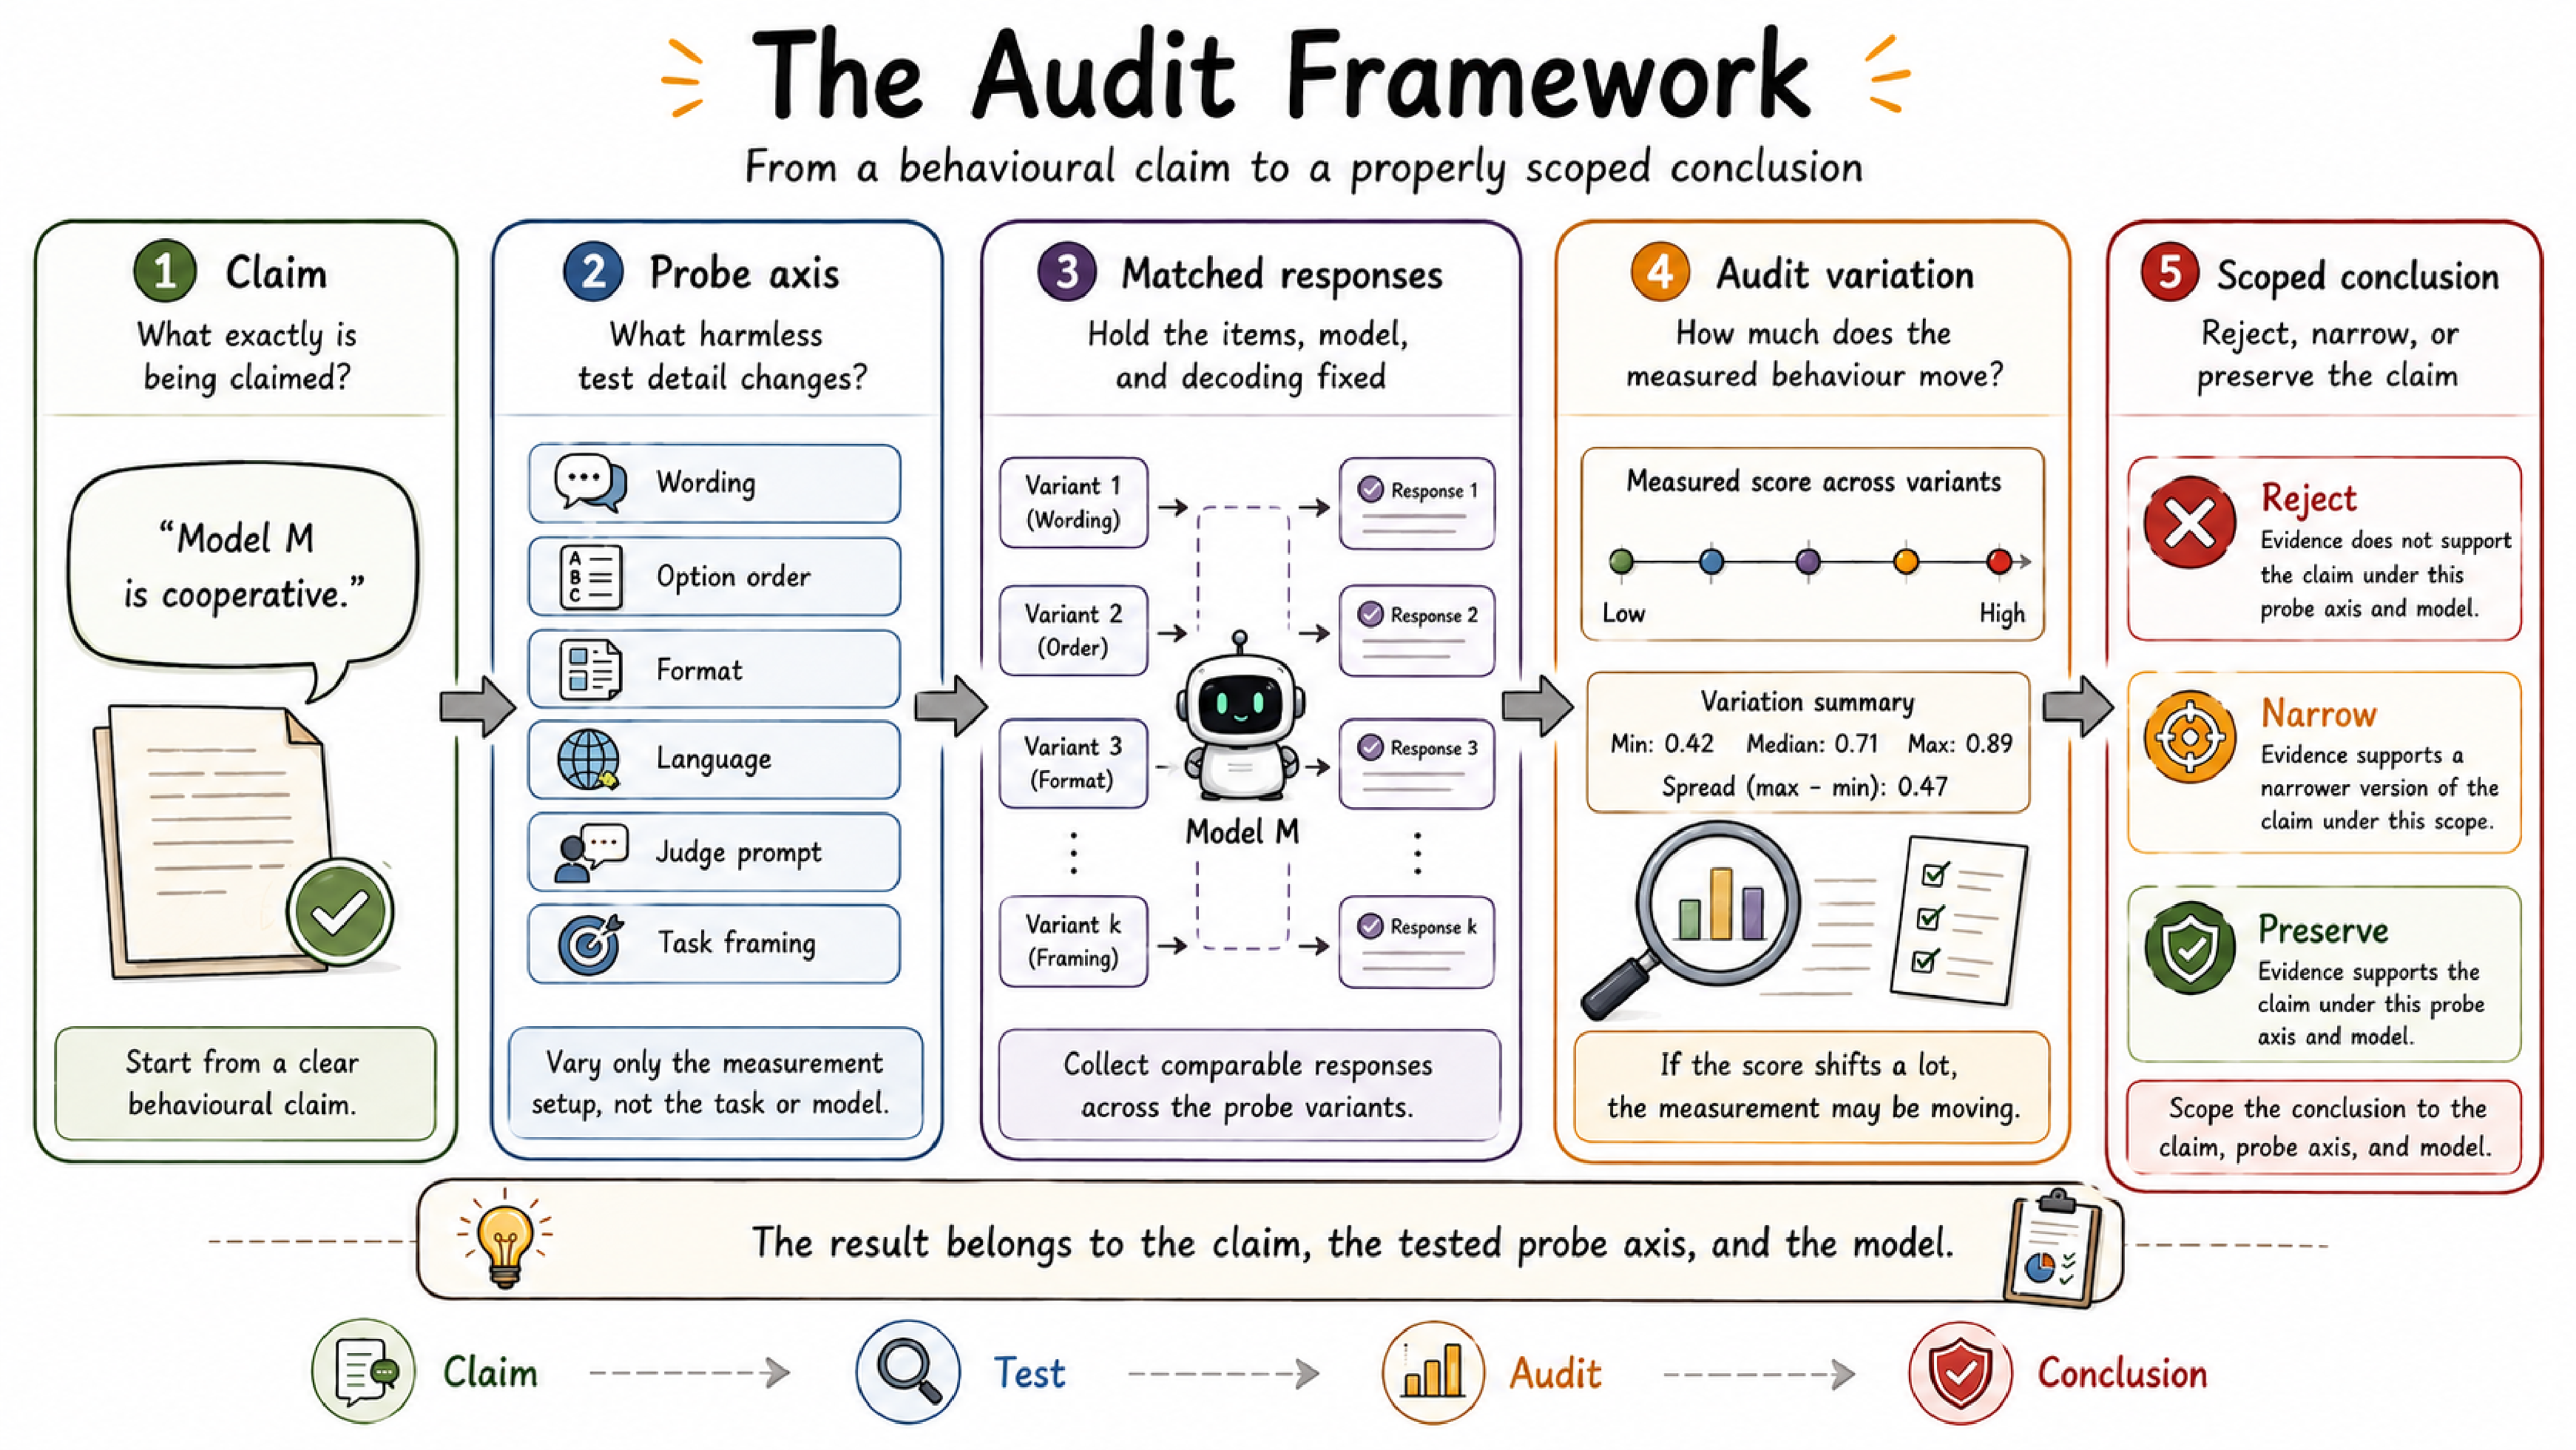
\includegraphics[width=0.98\textwidth]{figures/appendix/audit_framework.pdf}
\caption*{\small\textit{Conceptual illustration.} A visual guide to the claim-centred audit. The five stages mirror the
pipeline in Figure~\ref{fig:pipeline}: state a claim, declare the tested axis,
collect matched responses, audit variation, and scope the conclusion. The
numbers inside the illustration are placeholders, not reported estimates.}
\end{figure*}

The reporting standards of Section~\ref{sec:checklist} (Table~\ref{tab:checklist})
correspond to concrete statistical templates. \textbf{Reliability (T1, T2).} Fix an a priori pool of
prompts and formats before running anything and report the mean, standard
deviation, and range across it; where the design allows, partition the total
variance into a signal component (across items) and a perturbation component
(across formats, orders, and runs), and treat a behaviour whose perturbation
component dominates as not yet a finding. This decomposition is practical:
\citet{romanou2026brittlebench} find that perturbation-attributable variance
is roughly half of the total for most open-weight models, and that a single
meaning-preserving perturbation reorders the model ranking in $63\%$ of cases.
For order bias, report a \emph{signed} position-bias statistic with a
confidence interval over a pre-registered number of permutations, not an
accuracy averaged over a few orders. \textbf{Validity (T3, T4).} Report the
pass rate under a suite of meaning-preserving edits and adversarial
rephrasings and the stability of the result under at least two scoring
metrics; report sensitivity to framing alongside the equilibrium or
human-likeness score, so a reader can see how much of the verdict rests on the
scoring standard. \textbf{Generalizability (T5, T6).} Report worst-subgroup
performance and the full response distribution, and include at least one
information-asymmetric, multi-turn, or payoff-perturbed variant.

\subsection{What Counts as a Meaning-Preserving Edit}
\label{app:ppedit}

The reliability tier rests on perturbations that change the surface of a probe
without changing the question it asks, and that notion needs an operational
form or it becomes a matter of taste. We use a two-part test. An edit is
meaning-preserving if, first, a competent human respondent given both versions
would be expected to answer identically, and second, the edit does not add,
remove, or reweight any information the construct depends on. The first part is
checkable by annotation; the second is checkable by inspection of what changed.

Per task family this yields concrete permitted sets. For multiple-choice items:
separators, casing, whitespace, option labels, option order, and instruction
paraphrase. For open-ended generation: instruction paraphrase, system-prompt
placement, and output-format requests, but \emph{not} edits that change what is
being asked for. For games: payoff-preserving relabelling of actions and
players, and presentation order of the payoff matrix, but not framing words that
carry normative content, since those are a T4 manipulation rather than a T1 one.
For surveys and questionnaires: item order, response-option order, and
paraphrase, but not reverse-coding, which changes the item. The boundary case
worth naming is framing: a reframing word is meaning-preserving for the
decision problem but not for the construct if the construct is sensitive to
framing, which is exactly why we treat framing under T4 and format under T1.

\subsection{Estimators}
\label{app:estimators}

Three quantities make the standards above reproducible.

\textbf{Fragility fraction.} The fragility fraction $\phi$ estimates the share
of variance attributable to the probe. Run each of $n$ items under $K$ probe
variants (formats, orders, paraphrases, or seeds), then fit the two-way
random-effects decomposition $y_{ik}=\mu+a_i+b_k+(ab)_{ik}+\varepsilon_{ik}$.
The strict estimate is $\hat\phi_{\rm strict}=\hat\sigma^2_b/
\hat\sigma^2_{\rm total}$. The broad estimate also counts the item-by-probe
interaction: $\hat\phi_{\rm broad}=(\hat\sigma^2_b+\hat\sigma^2_{ab})/
\hat\sigma^2_{\rm total}$. Report a hierarchical bootstrap interval that
resamples both items and probes. Judge adequacy against the study's own
inversion-risk threshold and probe budget, not against a universal $0.5$ cutoff.

\textbf{Signed position bias.} For pairwise judging, present every pair in both
orders. Let $s_j$ be $1$ when position one wins, $0$ when position two wins, and
$1/2$ for a tie. Report $\hat\beta=\tfrac1N\sum_j(s_j-\tfrac12)$.
Here $\hat\beta=0$ means no positional preference; its sign
identifies the preferred position. Use a permutation confidence interval over a
pre-registered number of orderings rather than accuracy averaged over a few
orders. When the judge's error rates are known on a shared labelled set, a
plug-in correction \cite{angelopoulos2023ppi} converts the observed rate into an
unbiased estimate of the target rate.

\textbf{Probe-pool sizing.} To hold the standard error of the estimated spread
below a target $\epsilon$, use approximately
$K\gtrsim(z_{1-\alpha/2}\,\hat\sigma_b/\epsilon)^2$ probe variants. As a practical
starting point, use eight to ten formats and both orderings for each item. Use a
larger pool when $\hat\sigma_b$ is large or the claim is confirmatory.

\subsection{Outcomes That Are Not Binary}
\label{app:phiordinal}

The decomposition above is written for a binary or accuracy-valued outcome
because that is what the released corpora provide, but nothing in $\phi$ requires
it. For an \emph{ordinal} outcome, a Likert-style rating being the common case in
machine psychology, fit the same crossed random-effects structure through a
cumulative-link mixed model and read the variance components off the latent
scale; $\phi$ is then the probe share of latent variance and remains comparable
across instruments with different numbers of response categories, which a raw
score variance is not. For a \emph{continuous} outcome, such as a judge's scalar
rating, the linear model applies directly. For \emph{open-ended} generation there
is no outcome variable until one is defined, and that definition is itself a
measurement decision: whatever scalar the study reports, an embedding similarity,
a rubric score, a win rate, is the quantity to decompose, and the scoring
function must be inside the probe pool rather than outside it, since a rubric or
a judge is a probe. When the outcome is a rate estimated by a model judge, the
plug-in correction of Appendix~\ref{app:templates} should be applied before
decomposition, otherwise judge error inflates the residual and deflates $\phi$.

A practical caution for small pools. Method-of-moments components can be
negative in thin designs. We truncate them to zero only for display, report the
number truncated ($18/132$ cells in the harmonised analysis), and do not interpret
their point estimates without the hierarchical interval; truncation otherwise
biases $\phi$ upward. With fewer than six probe conditions we treat the point
estimate as exploratory, and with an unbalanced design prefer restricted maximum
likelihood or a Bayesian hierarchical fit. The bootstrap must resample both
items and probe conditions.

\subsection{What the Remedies Cost}
\label{app:cost}

The mitigations of Section~\ref{sec:checklist} are not free, and a reader
choosing among them needs the price. Expanding the probe pool is linear in
inference cost: $K$ formats multiply the evaluation budget by $K$, which is why
the sizing rule matters, and why the tolerable $\phi$ is stated as a function of
$K$ rather than as a constant. Balanced permutation for order bias doubles cost
for a pairwise judge, since each comparison is run in both directions, and this
is the cheapest high-value intervention available: it converts an unmeasured
prior into a signed statistic for a factor of two. Template ensembles cost the
same as the probe pool they average over and require no labels. Batch
calibration is essentially free, being a post-hoc transformation of scores
already computed. Judge calibration is the remedy with a human-labelling cost.
Its sample size must follow the required precision, power, and subgroup
coverage. Under stated sampling assumptions, a calibrated estimator can return
an interval with coverage. The variance decomposition itself
adds no inference cost at all, since it reuses outcomes the study already has,
and this is the reason we propose $\phi$ as the entry point: it is the one
diagnostic that is free to any study willing to record its probe-level results.

\textbf{Minimal probe pools.} ``Add more probes'' is not actionable
without a design, so we give three that a study can copy, each sized by the
threshold rule ($\phi^\ast\approx0.03$ at $K=1$, $0.17$ at $K=5$, $0.67$ at
$K=20$). The rule to size $K$ is to run a pilot on a tenth of the items, estimate
$\hat\phi$, and choose the smallest $K$ whose threshold exceeds it; a study
finding $\hat\phi\approx0.38$, as we do on dilemmas, needs roughly $K=10$ rather
than the one probe it was about to use.

For a \emph{forced-choice survey or questionnaire}, cross three
meaning-preserving paraphrases with both option orders in a $3\times2$ balanced
design ($K=6$, cost $6\times$), which is the MoralChoice design. Repeated
observations within each cell separate item-by-probe interaction from run noise;
if the
budget allows only $K=4$, a Latin square over four paraphrase-by-order cells
keeps both factors balanced and still separates their main effects, at the price
of confounding the interaction with the residual.

For a \emph{game or scenario study}, vary the factor the claim is not about:
two framings of the same payoff matrix crossed with two orderings of the action
list, plus a payoff-perturbed replicate ($K=5$), so that framing sensitivity and
order sensitivity are separately visible and the perturbed replicate doubles as
the T6 transfer probe.

For an \emph{LLM-as-judge evaluation}, the minimum is every comparison in both
presentation orders ($K=2$, cost $2\times$), which is what converts an unmeasured
prior into the signed $\hat\beta$; a fuller pool adds two rubric phrasings, giving
a $2\times2$ design ($K=4$) that separates position bias from rubric sensitivity,
and a gold-labelled slice sized for the desired precision and subgroup coverage
if a calibrated interval is required. In all three, probes should be sampled from the same pool the study
would defend as equivalent, since $\phi$ is defined relative to that pool and a
pool chosen to be easy will understate fragility.

\subsection{Guarding Against Probe-Pool Gaming}
\label{app:poolgaming}

A warning is not a safeguard when authors benefit from a small value. We use
three. First, define the admissible axes and the equivalence rule before seeing
outputs: for forced choice, at minimum paraphrase crossed with order; for games,
payoff-preserving action and player relabellings; for judging, both candidate
orders and at least two rubric phrasings. Second, release every probe-level cell
and report $\phi$ for the full pool and for nested random subsets. Third, report
the half-pool adequacy ratio
$A=\operatorname{median}_S\{\hat\phi(S_{K/2})/\hat\phi(S_K)\}$. Values near one
mean that adding the held-out half no longer changes the estimate materially;
values below one flag an unsaturated pool, without pretending that one cutoff is
universal.

The exploit is measurable on our own data. Across MoralChoice cells, choosing
two of the six conditions moves the median attainable strict $\phi$ from $0$ to
$0.213$; with five conditions, $25\%$ of cells admit a misleadingly stable subset on
either side of the paper's $K=5$ threshold. The half-pool ratio is $0.89$ (IQR
$[0.71,1.03]$) for MoralChoice and $1.01$ ($[0.99,1.02]$) for PromptEval. These
numbers do not certify a canonical pool. They show why preregistration, a
versioned task-family pool, subset curves, and full release are all required:
the last two let a reader detect gaming even when the first two fail.

\subsection{When an Order Effect Is Part of the Construct}
\label{app:t2construct}

Placing order effects under reliability invites a sharp objection. In a genuine
preference task, the salience of an option may be part of what preference
\emph{means} for the system being measured, in which case treating position
sensitivity as pure noise assumes away the phenomenon. Human choice research
takes this seriously, and so should we.

Our answer is that reliability is relative to the claim, not to the
measurement. The same measured quantity can be noise for one construct and
signal for another, and the audit asks which construct is being claimed.
Consider the judge data above. If the claim is about \emph{answer quality},
presentation order is irrelevant to it by construction, a well-posed quality
measure cannot depend on which answer was typed first, and the $16.3\%$
disagreement is measurement error to be reported and reduced. If instead the
claim is about \emph{the judge itself}, that same position effect is the
construct: it is stable, it has a sign, it reproduces across datasets, and it
predicts held-out behaviour, which is exactly why ``language-model judges carry
a position bias'' passes all three tiers in Appendix~\ref{app:casestudy} while
almost no absolute claim does.

The test that separates the two cases is the second condition of
Appendix~\ref{app:construct}, behavioural entailment. A position effect that is
part of a preference construct should predict something else about the system
that was not used to measure it. A position effect that predicts nothing beyond
itself is a response tendency of the instrument. This is a testable distinction
rather than a matter of taste, and we would rather state it than let the
placement of T2 rest on stipulation. Where a study genuinely intends option
salience as part of its construct, the requirement is not that it abandon the
claim but that it say so in advance and score against a target that includes
salience, which is the T4 discipline of Appendix~\ref{app:t4template}.

\section{Estimating the Fragility Fraction}
\label{app:phistats}

This appendix gathers the statistical machinery behind the severity scale of
Section~\ref{sec:checklist}: how $\phi$ is estimated on real corpora, how its
threshold is derived, how wide its intervals are, and how it relates to a
different variance decomposition in the literature.

\begin{figure*}[t]
\centering
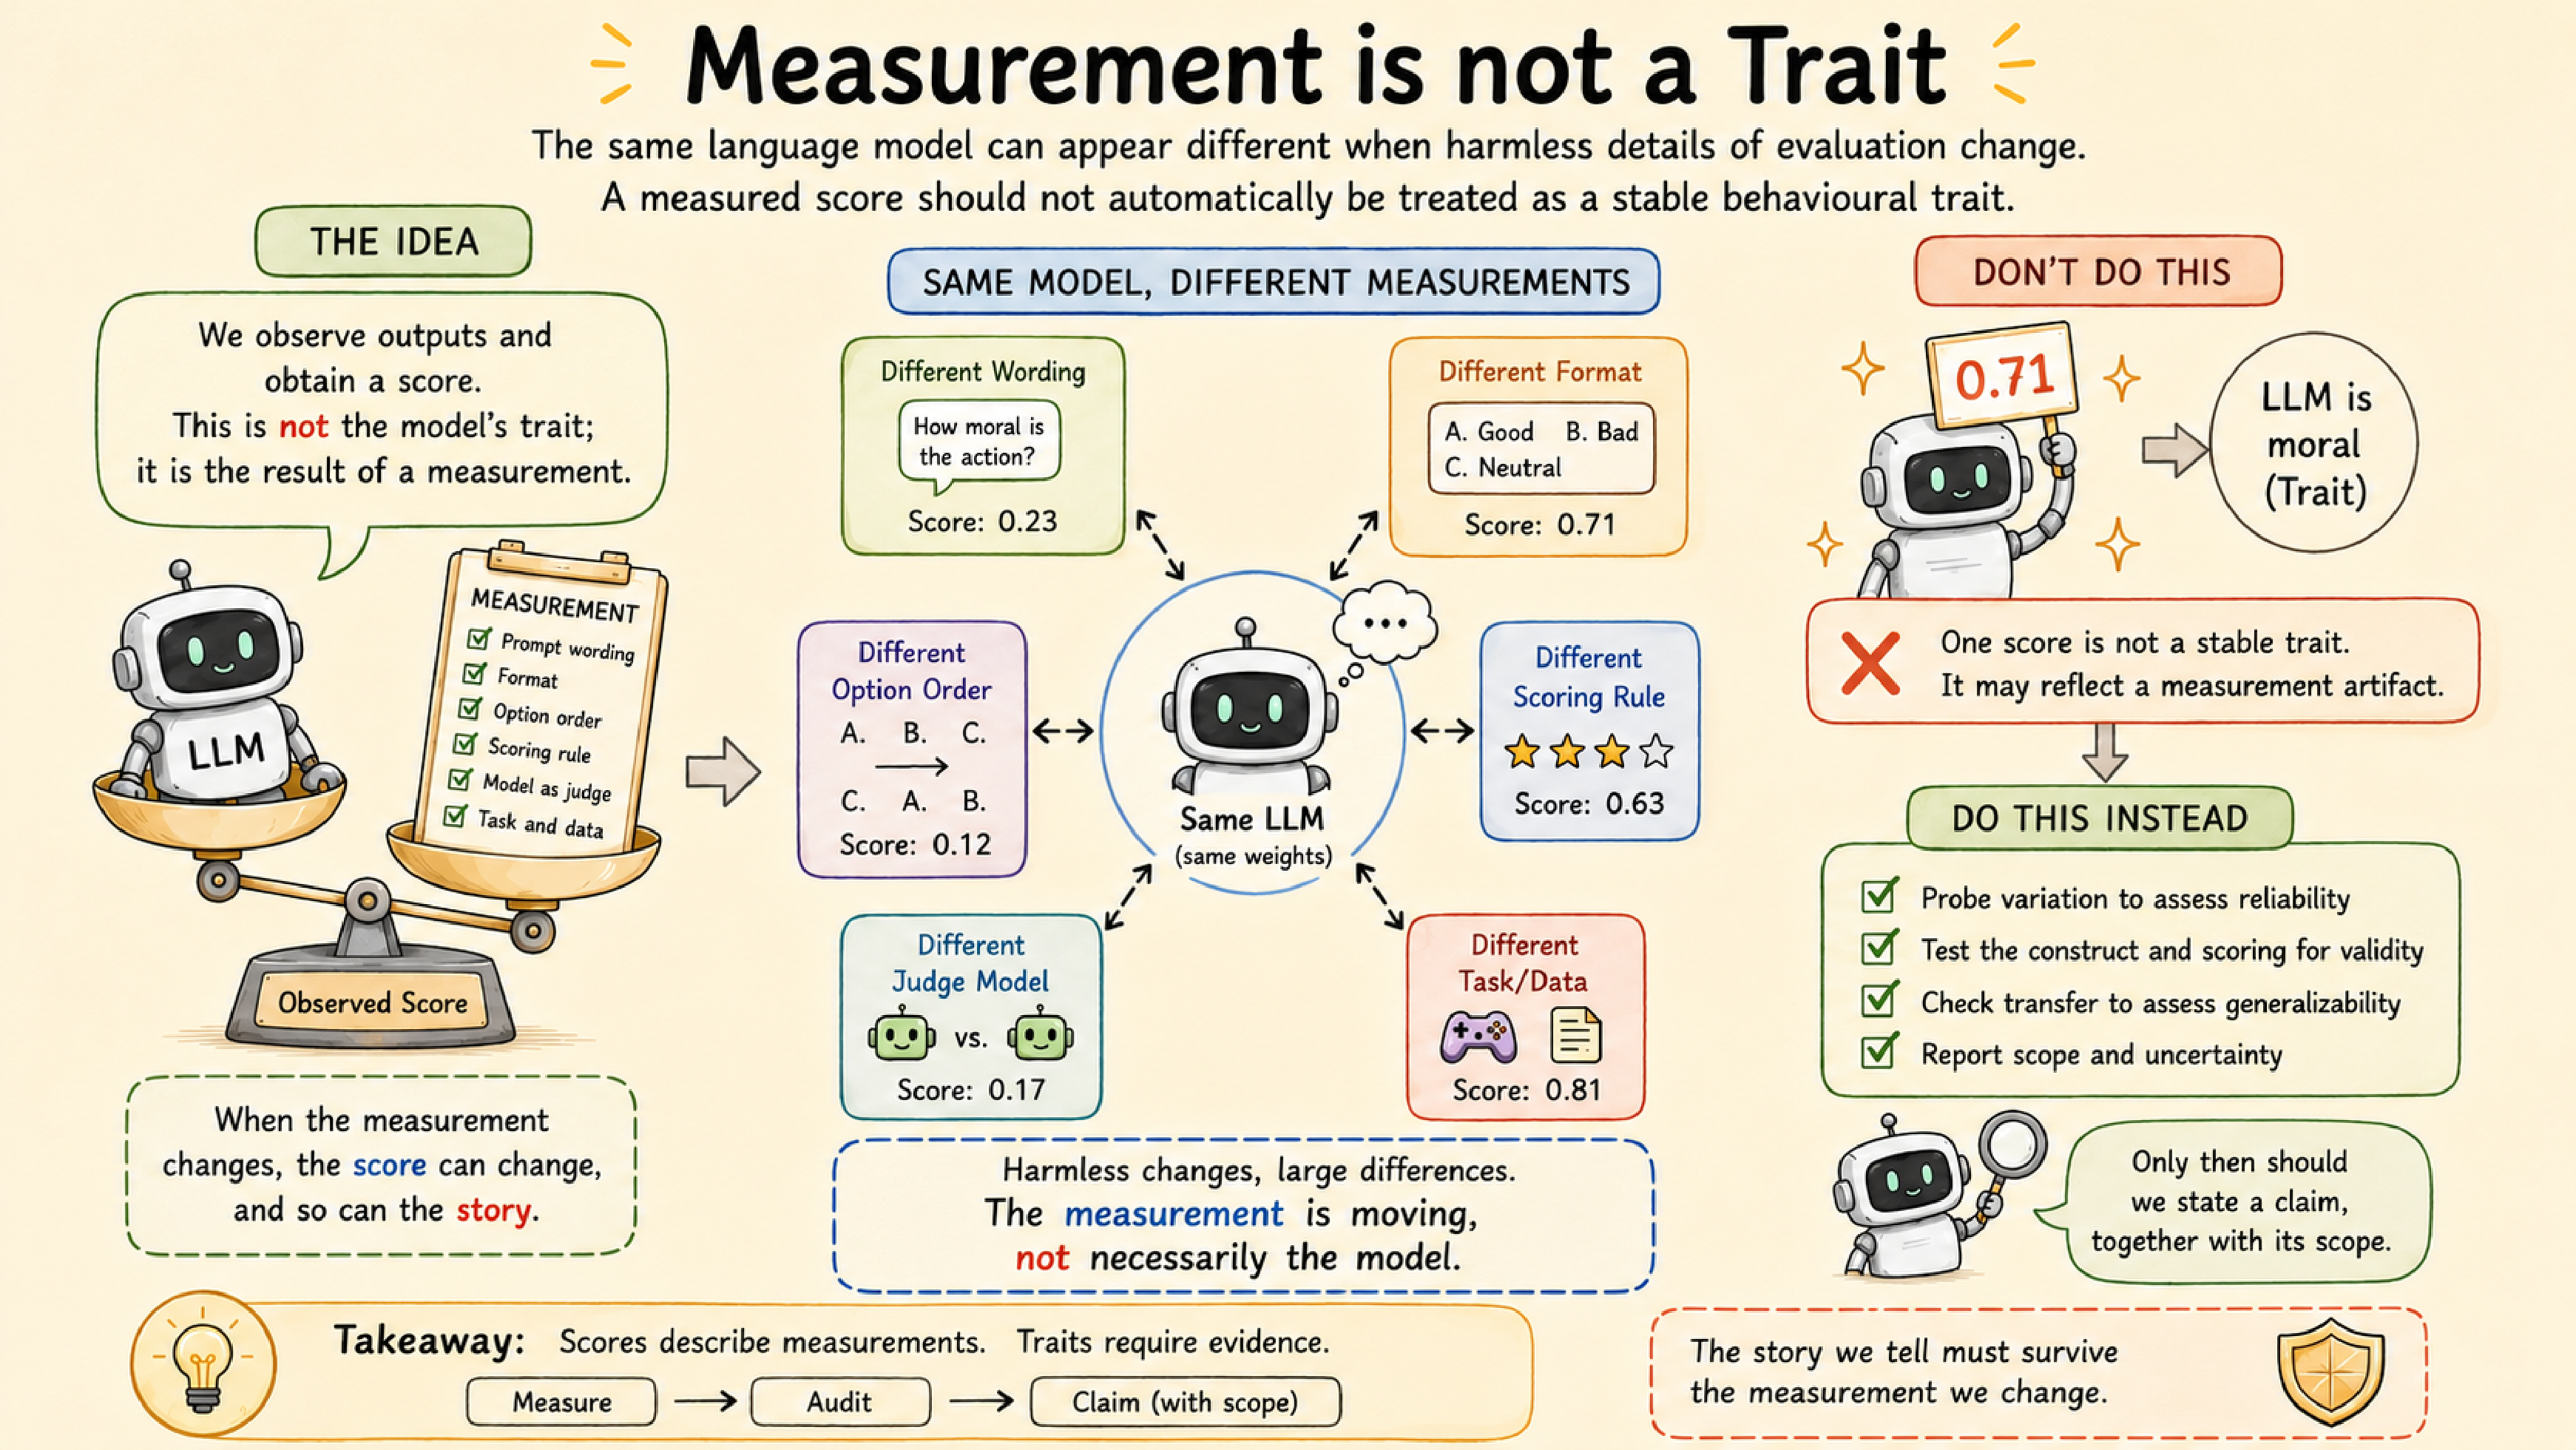
\includegraphics[width=0.98\textwidth]{figures/appendix/measurement_is_not_a_trait.pdf}
\caption*{\small\textit{Conceptual illustration.} A score is produced by a measurement
procedure. Changing a prompt, response format, scoring rule, judge, or task can
change the score. This does not by itself disprove a behavioural claim; it shows
why the claim needs reliability, validity, and transfer evidence. The displayed
scores are illustrative placeholders.}
\end{figure*}

\subsection{Estimating $\phi$ on Released Data}
\label{app:phiempirical}

To show that $\phi$ is computable rather than merely definable, we estimate it on
two released corpora chosen to sit on opposite sides of the survey's distinction
(Figure~\ref{fig:phiforest}):
one capability benchmark with a verifiable answer, and one behavioural probe
where the quantity of interest is a preference.

\textbf{A capability benchmark: the negative control.} PromptEval
\cite{polo2024efficient} records the correctness of $15$ models on $57$ MMLU
subjects under $100$ meaning-preserving prompt templates ($8.55$M binary
outcomes). The category-level summary below comes from that full extraction.
The packaged matched-item core currently contains $84$ matrices from $7$ models
and $12$ subjects; Appendix~\ref{app:harmonised} reports only the $47$ cells in
that subset with enough mid-difficulty items. Reducing each (subject, model) cell to $100$ template-level
accuracies and decomposing at the level a claim is made, the reported accuracy,
gives a median $\hat\phi=0.001$ when subject is the signal and $\hat\phi=0.003$
when \emph{model identity} is the signal. In none of the $57$ subjects does
template variance exceed model variance; one model holds rank~1 under all $100$
templates and no model moves more than three rank positions. Per cell the
template-induced accuracy spread is still a median of $8.9$ points, the quantity
single-probe reporting hides, but the ordering survives. Where measurement is
well posed, $\phi$ correctly reports low fragility.

\textbf{A behavioural probe: the positive case.} MoralChoice
\cite{scherrer2023evaluating} releases the responses of $28$ models to moral
scenarios under a fully crossed probe design: three question forms, both option
orderings, and five samples at temperature~$1$. We analyse $12$ models spanning
six developers, on both the low-ambiguity set ($687$ scenarios with a
commonsense-moral action) and the high-ambiguity set ($680$ genuine dilemmas,
where the measured quantity is a preference and a stable-trait claim is exactly
what a study would report). Writing $y=\mathbf{1}[\text{model picks action~1}]$,
we average over samples to obtain $y[\text{scenario},\text{condition}]$ for the
six format-by-order conditions and apply the same two-way decomposition. We
report $\phi_{\text{strict}}$, which counts only the main effect of the probe
condition, and $\phi_{\text{broad}}$, which also counts the
scenario-by-condition interaction, since a probe that changes the answer
differently for each scenario is still probe dependence. Repeats estimate the
run-noise contribution to the residual. We remove that contribution from the
broad numerator but retain it in total measured variance.

The behavioural picture is qualitatively different from the capability one. On
the genuine dilemmas the median is $\hat\phi_{\text{strict}}=0.15$ and
$\hat\phi_{\text{broad}}=0.38$, with $2$ of $12$ models above $0.5$ on the broad
measure; on the low-ambiguity set the medians are $0.32$ and $0.67$. A model's
measured moral preference moves across probe conditions by a median of $34$ and
a maximum of $94$ percentage points. Refusal and invalid rates are below $1\%$,
and are excluded before forming cell means; we then require a complete
scenario-by-condition matrix, rather than coding a refusal as either action.
Thus the contrast concerns conditional choices, while refusal is reported as a
separate T3 outcome. Juxtaposing the broad behavioural median with
the capability benchmark's $0.003$ would suggest a roughly fifty-fold contrast,
but that comparison mixes estimands, aggregation levels, pool sizes, and
estimators. We retain neither the ratio nor the category-level reading;
Appendix~\ref{app:harmonised} rebuilds the comparison on one scale.

The variance also changes shape with the question. On low-ambiguity items, where
a clear answer exists, the format term dominates
($\hat\sigma^2_{\text{format}}=0.025$ against
$\hat\sigma^2_{\text{order}}=0.0005$): the probe determines whether the model
finds the answer. On genuine dilemmas the format term collapses
($0.002$) and the option-order and sampling terms take over
($0.014$ and $0.119$): with no stable preference to report, what is measured is
the presentation prior and the sampling noise. This is T2 and T5 acting exactly
as Section~\ref{sec:checklist} describes, and it is visible only because the
design crosses the factors. Models differ sharply: GPT-4 is among the less
probe-dependent models ($\hat\phi_{\text{broad}}=0.21$), while
text-davinci-003 is the most probe-dependent ($0.73$, with the $94$-point
spread). Fragility is a property of the model-probe pair rather than of the task
alone.

\begin{figure*}[t]
\centering
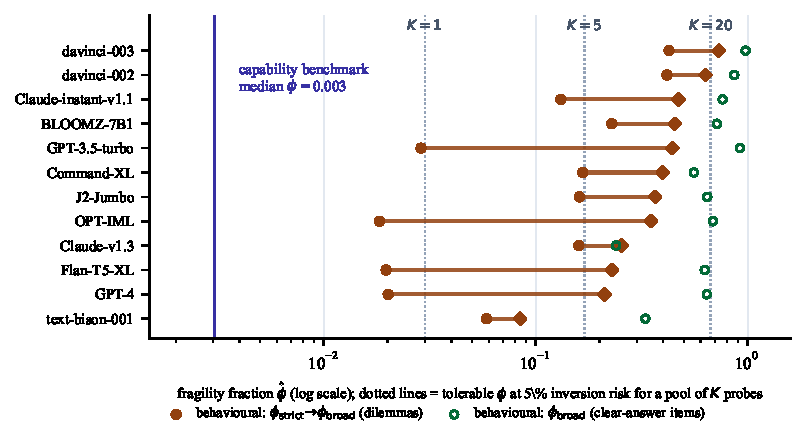
\includegraphics[width=0.93\textwidth]{figures/core/phi_forest.pdf}
\caption{The fragility fraction across the two corpora, on a log scale. The
vertical line is the median $\hat\phi$ on a capability benchmark with a
verifiable answer ($0.003$; PromptEval, $15$ models, $100$ templates). Each row
is a model on the behavioural probe (MoralChoice): the bar spans
$\hat\phi_{\text{strict}}$ to $\hat\phi_{\text{broad}}$ on the genuine dilemmas,
and the open circle is $\hat\phi_{\text{broad}}$ on the clear-answer items.
This is a descriptive overview, not a like-for-like cross-corpus comparison:
the probes, item populations, replication, and estimands differ. The matched
strict comparison and its limitations are in Appendix~\ref{app:harmonised}.
Dotted lines are conditional inversion-risk illustrations, not universal
thresholds (Appendix~\ref{app:phithreshold}).}
\label{fig:phiforest}
\end{figure*}

\subsection{Making the Comparison Like for Like}
\label{app:harmonised}

The comparison in the previous subsection is not yet apples to apples, and the
gap between the two numbers is not the only thing that differs between them. Put
plainly, $\hat\phi=0.003$ and $\hat\phi_{\text{broad}}=0.38$ differ in five ways
at once, of which only the last is the one the claim is about:

\begin{itemize}\itemsep2pt
\item \textbf{Aggregation level.} The capability figure was computed over
      subject-level accuracies, the behavioural one over scenario-level
      outcomes. Aggregating to subjects averages away within-subject noise and
      inflates the between-item term in the denominator, which deflates $\phi$
      mechanically.
\item \textbf{Estimand.} $0.003$ is $\phi_{\text{strict}}$ and $0.38$ is
      $\phi_{\text{broad}}$. These are different quantities.
\item \textbf{Estimator.} The capability path used a raw sum-of-squares share;
      the behavioural path used method-of-moments variance components, which
      subtract the residual mean square. On PromptEval the two disagree by a
      factor of seven ($0.0014$ against $0.0002$).
\item \textbf{Probe count.} $K=100$ templates against $K=6$ conditions.
\item \textbf{Difficulty filtering.} Applied to one corpus and not the other.
\end{itemize}

We therefore reduce every corpus to the same object: an items-by-conditions
matrix with one observation per cell, item being the unit a stable-trait claim
is read off, and one estimator throughout. Table~\ref{tab:harmonised} reports the
result.

One asymmetry cannot be removed and should be stated rather than smoothed over.
$\phi_{\text{strict}}$ is comparable across corpora. $\phi_{\text{broad}}$ is not,
when one corpus has replicates and another does not: with a single sample per
cell and a binary outcome, the Bernoulli variance $p(1-p)$ cannot be separated
from the item-by-probe interaction, so on PromptEval $\phi_{\text{broad}}$ is not
identifiable at all. We report $\phi_{\text{strict}}$ as the comparable quantity,
and $\phi_{\text{broad}}$ only where replicates make it estimable, netting the
sampling variance out of the interaction numerator while retaining it in the
denominator.

\begin{table}[H]
\centering
\scriptsize
\setlength{\tabcolsep}{2.5pt}
\begin{adjustbox}{max width=\columnwidth}
\begin{tabular}{@{}lrrr@{}}
\toprule
\rowcolor{cardblue!55}
\textbf{Corpus and claim} & \textbf{all} & \textbf{mid, full $K$} & \textbf{mid, $K=6$} \\
\midrule
Capability (MMLU)          & $0.0002$ & $0.0119$ & $0.0069$ \\
\rowcolor{leafbg}
Behavioural, dilemmas      & $0.0619$ & $0.1439$ & $0.1439$ \\
Behavioural, clear answer  & $0.1428$ & $0.3059$ & $0.3059$ \\
\bottomrule
\end{tabular}
\end{adjustbox}
\caption{Median $\hat\phi_{\text{strict}}$ on a common item-by-condition
object and method-of-moments estimator. \textbf{all} uses every item;
\textbf{mid} keeps items whose mean score lies in $(0.2,0.8)$; and $K=6$
subsamples PromptEval to six templates, with the median over $200$ draws.
The matched subset contains $47$ PromptEval subject-model cells and all $12$
MoralChoice models; MoralChoice has $680$ dilemmas and $687$ clear-answer
scenarios before complete-case filtering.
This controls aggregation level and probe count, but does not make task meaning,
outcome link, or item population identical. The artifact reports the full
template-draw distribution; the point values are illustrative rather than a
universal cross-corpus ratio.}
\label{tab:harmonised}
\end{table}

The direction survives: strict $\phi$ is larger on the dilemmas than on the
capability setting under this common estimator. We do not treat its numerical
ratio as a cross-corpus constant. Difficulty filtering removes $46\%$ of MMLU
items against $9\%$ of dilemmas, so it raises the capability value more than the
behavioural one; template subsampling adds further uncertainty. The artifact
therefore reports the distribution over template draws and uses this table only
as a claim- and axis-specific illustration. Across $200$ template draws, the
illustrative dilemma-to-capability ratio has median $20.9$ and central $95\%$
range $[10.9,68.6]$, which is why the abstract reports direction rather than a
fixed multiplier. Method-of-moments components were clamped at zero in $18$ of
$132$ cells, which can bias $\phi$ upward in thin pools and is another reason
not to generalise a point ratio.

\subsection{Exploratory Companion Analysis: Is High $\phi$ Just an Artefact of
Choosing Dilemmas?}
\label{app:positivecontrol}

\textbf{Release status.} This subsection uses a companion-project matrix that
is not yet portable in the public artifact. It is exploratory and is not used
for any abstract, main-text, or load-bearing quantitative claim. We retain the
analysis specification to show how a future licensed release can test the
denominator objection.

There is a serious objection to the MoralChoice illustration. A moral dilemma is, by
construction, a scenario built to have no stable answer. If the between-item
signal is near zero by design, $\phi$'s denominator collapses and a large $\phi$
says nothing about behavioural probes in general. The portable MoralChoice data
address the denominator directly; the remaining checks below are exploratory
until their source matrices can be released.

\textbf{The denominator, printed.} $\phi$ is a ratio, so the claim can be checked
directly rather than by proxy. On the dilemmas $\hat\sigma^2_{\text{item}}=0.064$
and the split-half reliability of the item profile across probe conditions is
$0.76$: the ordering of scenarios is a real, reproducible signal, not noise. The
set whose denominator actually collapses is the \emph{clear-answer} set
($\hat\sigma^2_{\text{item}}=0.006$, split-half $0.26$), because models answer
almost all of those items the same way and there is no room left to vary.

\textbf{Paired within-model comparison.} MoralChoice ships both item sets, built
by the same authors, asked of the same twelve models under the same six
conditions. The collapse story predicts $\phi$ far lower on the clear-answer set.
It is not lower: median $0.14$ against $0.06$ on the dilemmas, higher in $8$ of
$12$ models (Wilcoxon signed-rank $p=0.052$).

\textbf{Exploratory out-of-sample contrast.} A stronger version of the
objection would ask for a behavioural corpus where a large disposition signal is
\emph{expected}. Moral Machine style autonomous-vehicle dilemmas supply one: the
preference for sparing humans over pets and more lives over fewer are among the
largest and most cross-nationally stable preferences ever measured on people
($77.8$ and $74.4$ on a scale where $50$ is indifference, between-country
standard deviations $6.1$ and $2.6$). We re-analyse a pre-existing crossed run of
$310$ such items posed in $20$ country-language variants to eleven models, with a
continuous outcome. Two constant-side models were excluded by a criterion fixed
before inspecting $\phi$, leaving nine models for the positive control. This is a
new between-item-normalised analysis of existing outputs, not a reuse of the
companion project's estimand. Its input matrix is not yet in the public
artifact, so the numerical comparison is illustrative rather than evidence for
the paper's central conclusion.

In this exploratory matrix, the item signal is unambiguous
($\hat\sigma^2_{\text{item}}=0.079$, split-half $0.97$), and yet
$\hat\phi_{\text{strict}}$ on the \emph{language} axis is $0.0005$, with a
hierarchical interval of width $0.008$: translating the dilemma into twenty
languages barely moves the reported preference. On the $35$ left/right-paired
comparisons, expanding the pool to language by side order gives
$\hat\phi_{\text{strict}}=0.30$. So a high $\phi$ is not
a property of behavioural measurement as a category. It is a property of the
triple (claim, probe axis, model), and a survey that reports one number for
``behavioural probes'' is doing the thing this survey warns against. Where the
body contrasts capability with behavioural fragility, the axis that carries it is
presentation order, not paraphrase and not translation.

\subsection{Why Strict $\phi$ Is Not Enough}
\label{app:strictbroad}

\begin{figure*}[t]
\centering
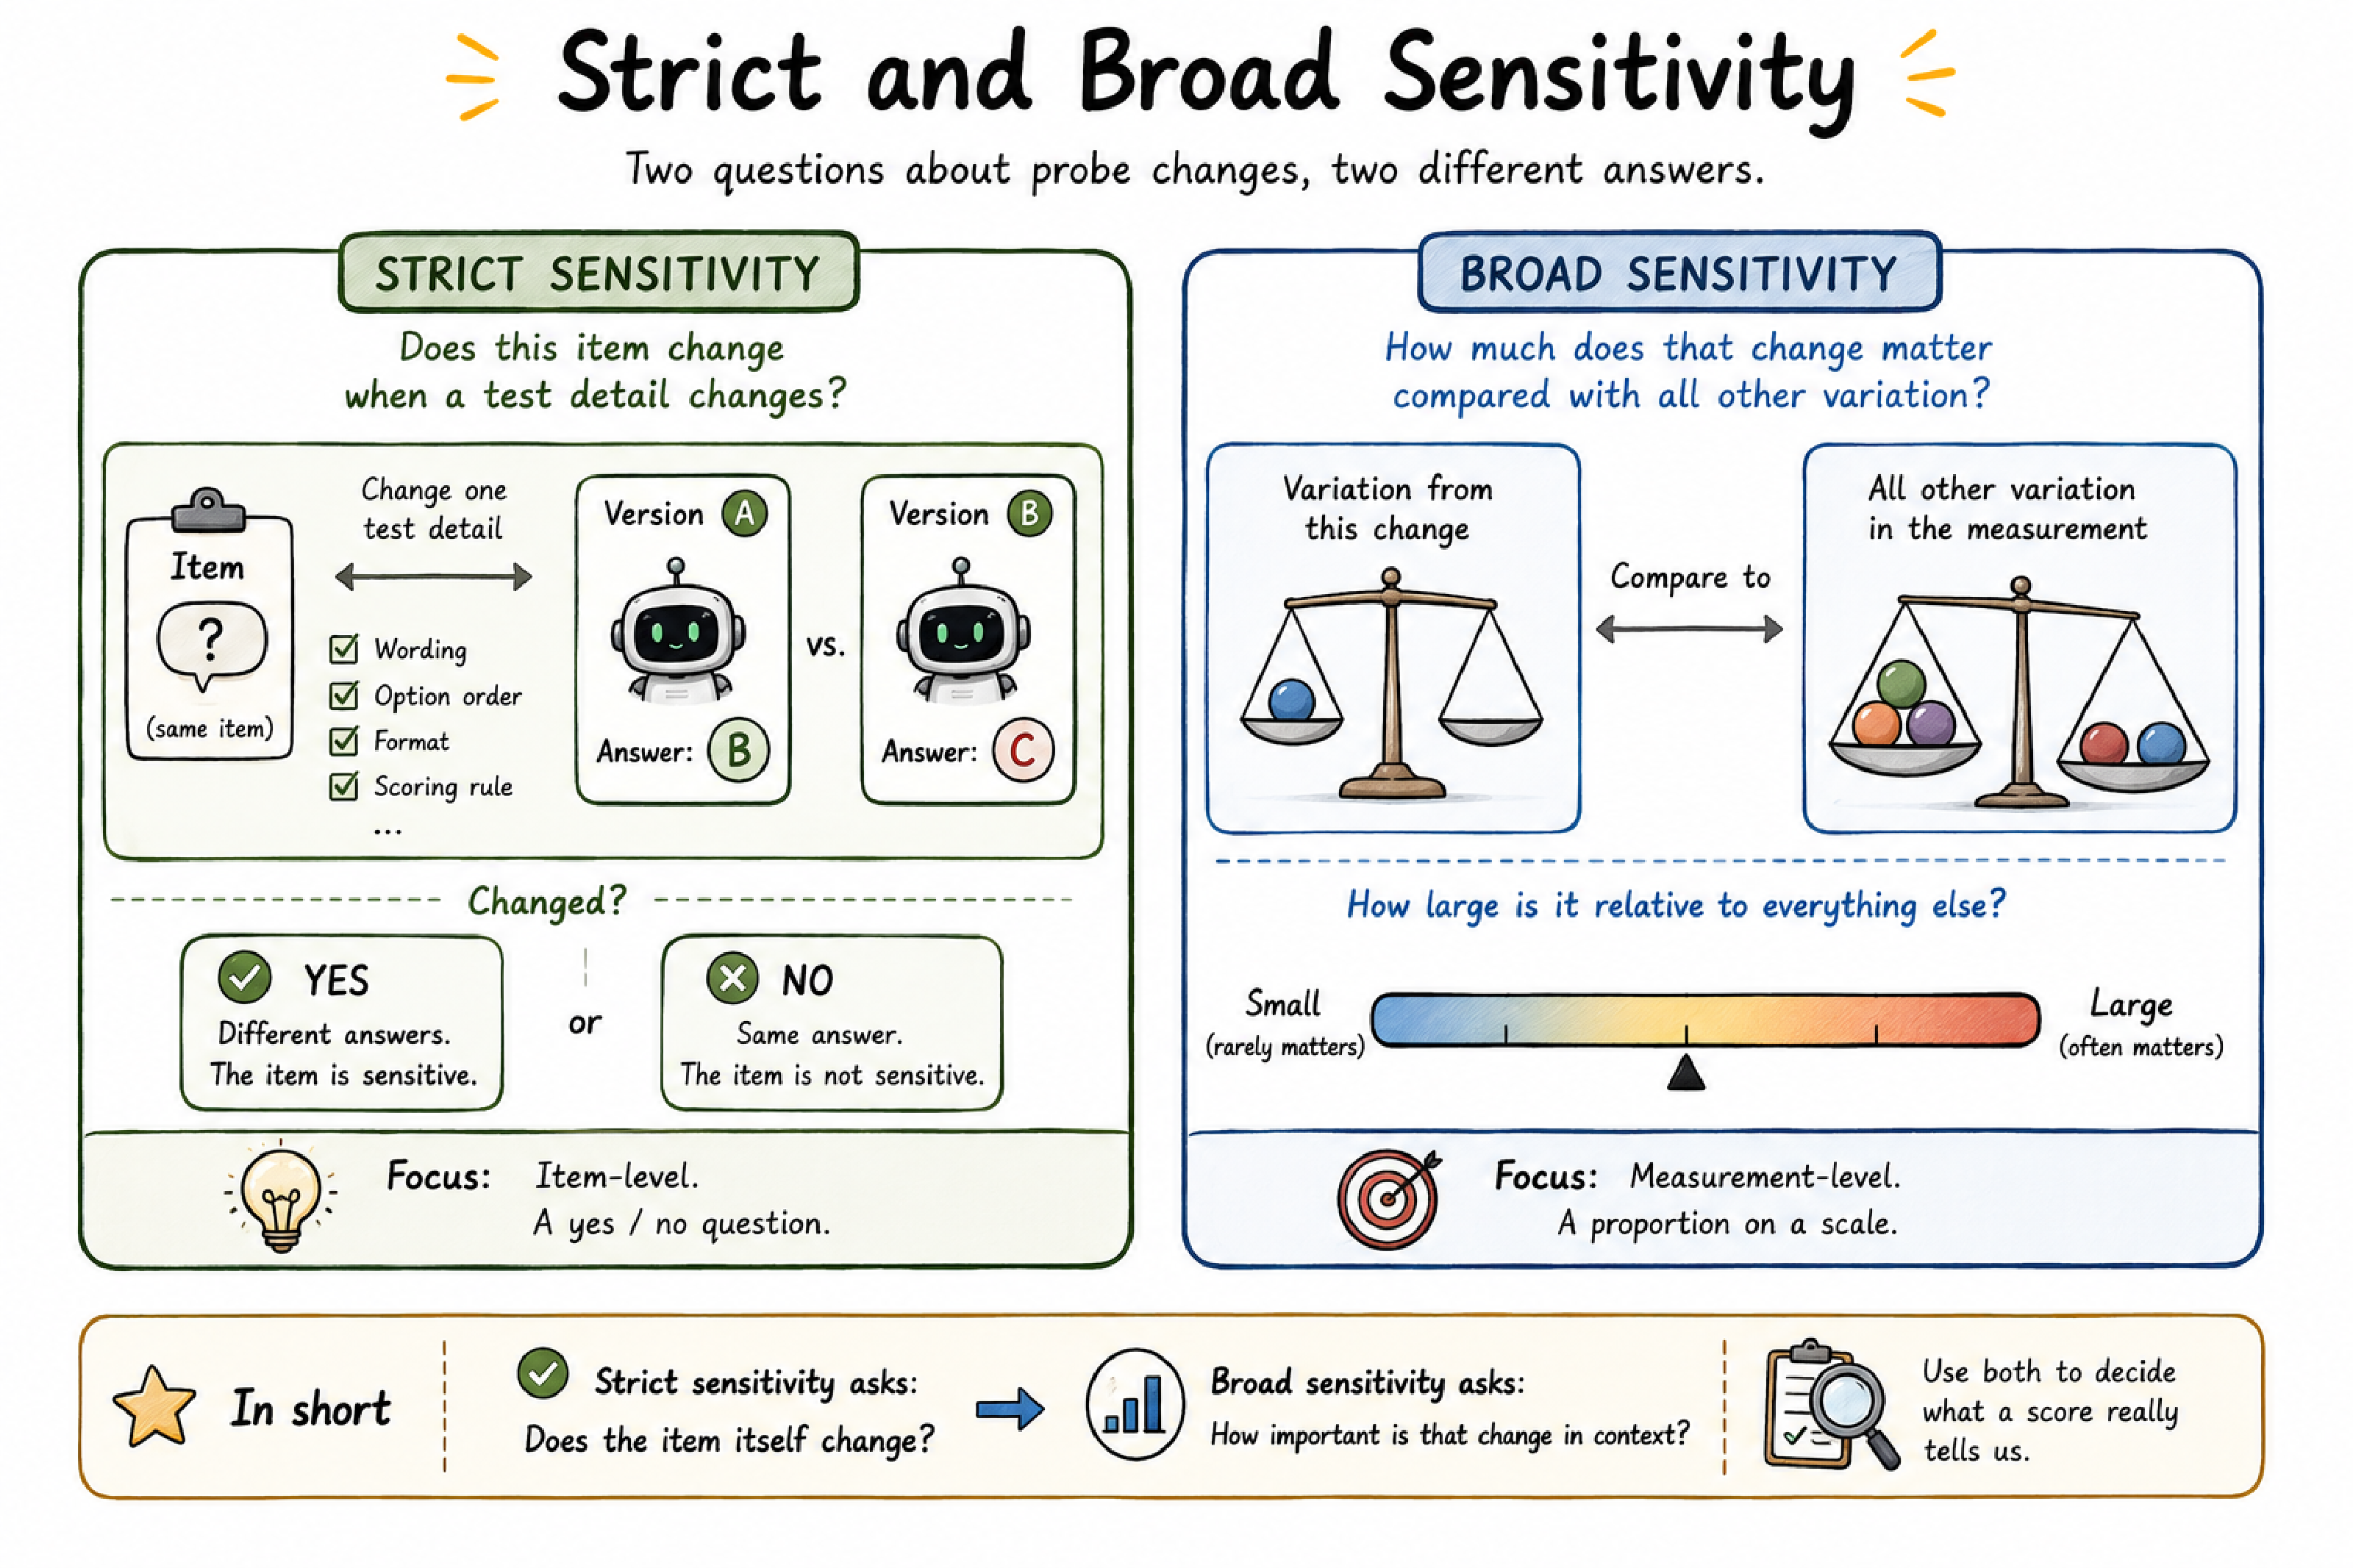
\includegraphics[width=0.98\textwidth]{figures/appendix/strict_vs_broad_sensitivity.pdf}
\caption*{\small\textit{Conceptual illustration.} An intuition for strict and broad sensitivity. Strict $\phi$ attributes
variation to the probe main effect; broad $\phi$ also includes the
item-by-probe interaction. The left panel is an intuitive item-level metaphor,
not the formal definition of strict $\phi$, which remains a variance fraction.}
\end{figure*}

The exploratory companion analyses also illustrate something the single-corpus
analysis could not establish.
On the language axis $\hat\phi_{\text{strict}}=0.0005$ while
$\hat\phi_{\text{broad}}=0.41$: translation does not move the average at all and
still changes the answer item by item. The same dissociation appears on a fourth
corpus, a cultural-knowledge benchmark under a full four-rotation sweep of the
option order ($1226$ items, one model, gold-scored). There
$\hat\phi_{\text{strict}}=0.000$ with a hierarchical interval of
$[0.000,0.001]$, accuracy by rotation is flat to within one point
($0.705$ to $0.717$), and yet $26.8\%$ of items change their predicted answer
when the options are rotated.

These exploratory examples illustrate a possible pattern: a probe axis can leave
the aggregate untouched and still scramble per-item conclusions. The practical
consequence is the reason
Eq.~\ref{eq:phimodel} keeps the interaction term. Any index or implementation
built only on the probe main effect understates fragility whenever the probe
helps some items and hurts others. POSIX-style itemwise spreads can see that
interaction; a corpus-level mean shift cannot. The distinction, not a blanket
claim that every competing index fails, is the head-to-head result.

\subsection{Open-Ended Generation}
\label{app:phiopen}

\begin{figure*}[t]
\centering
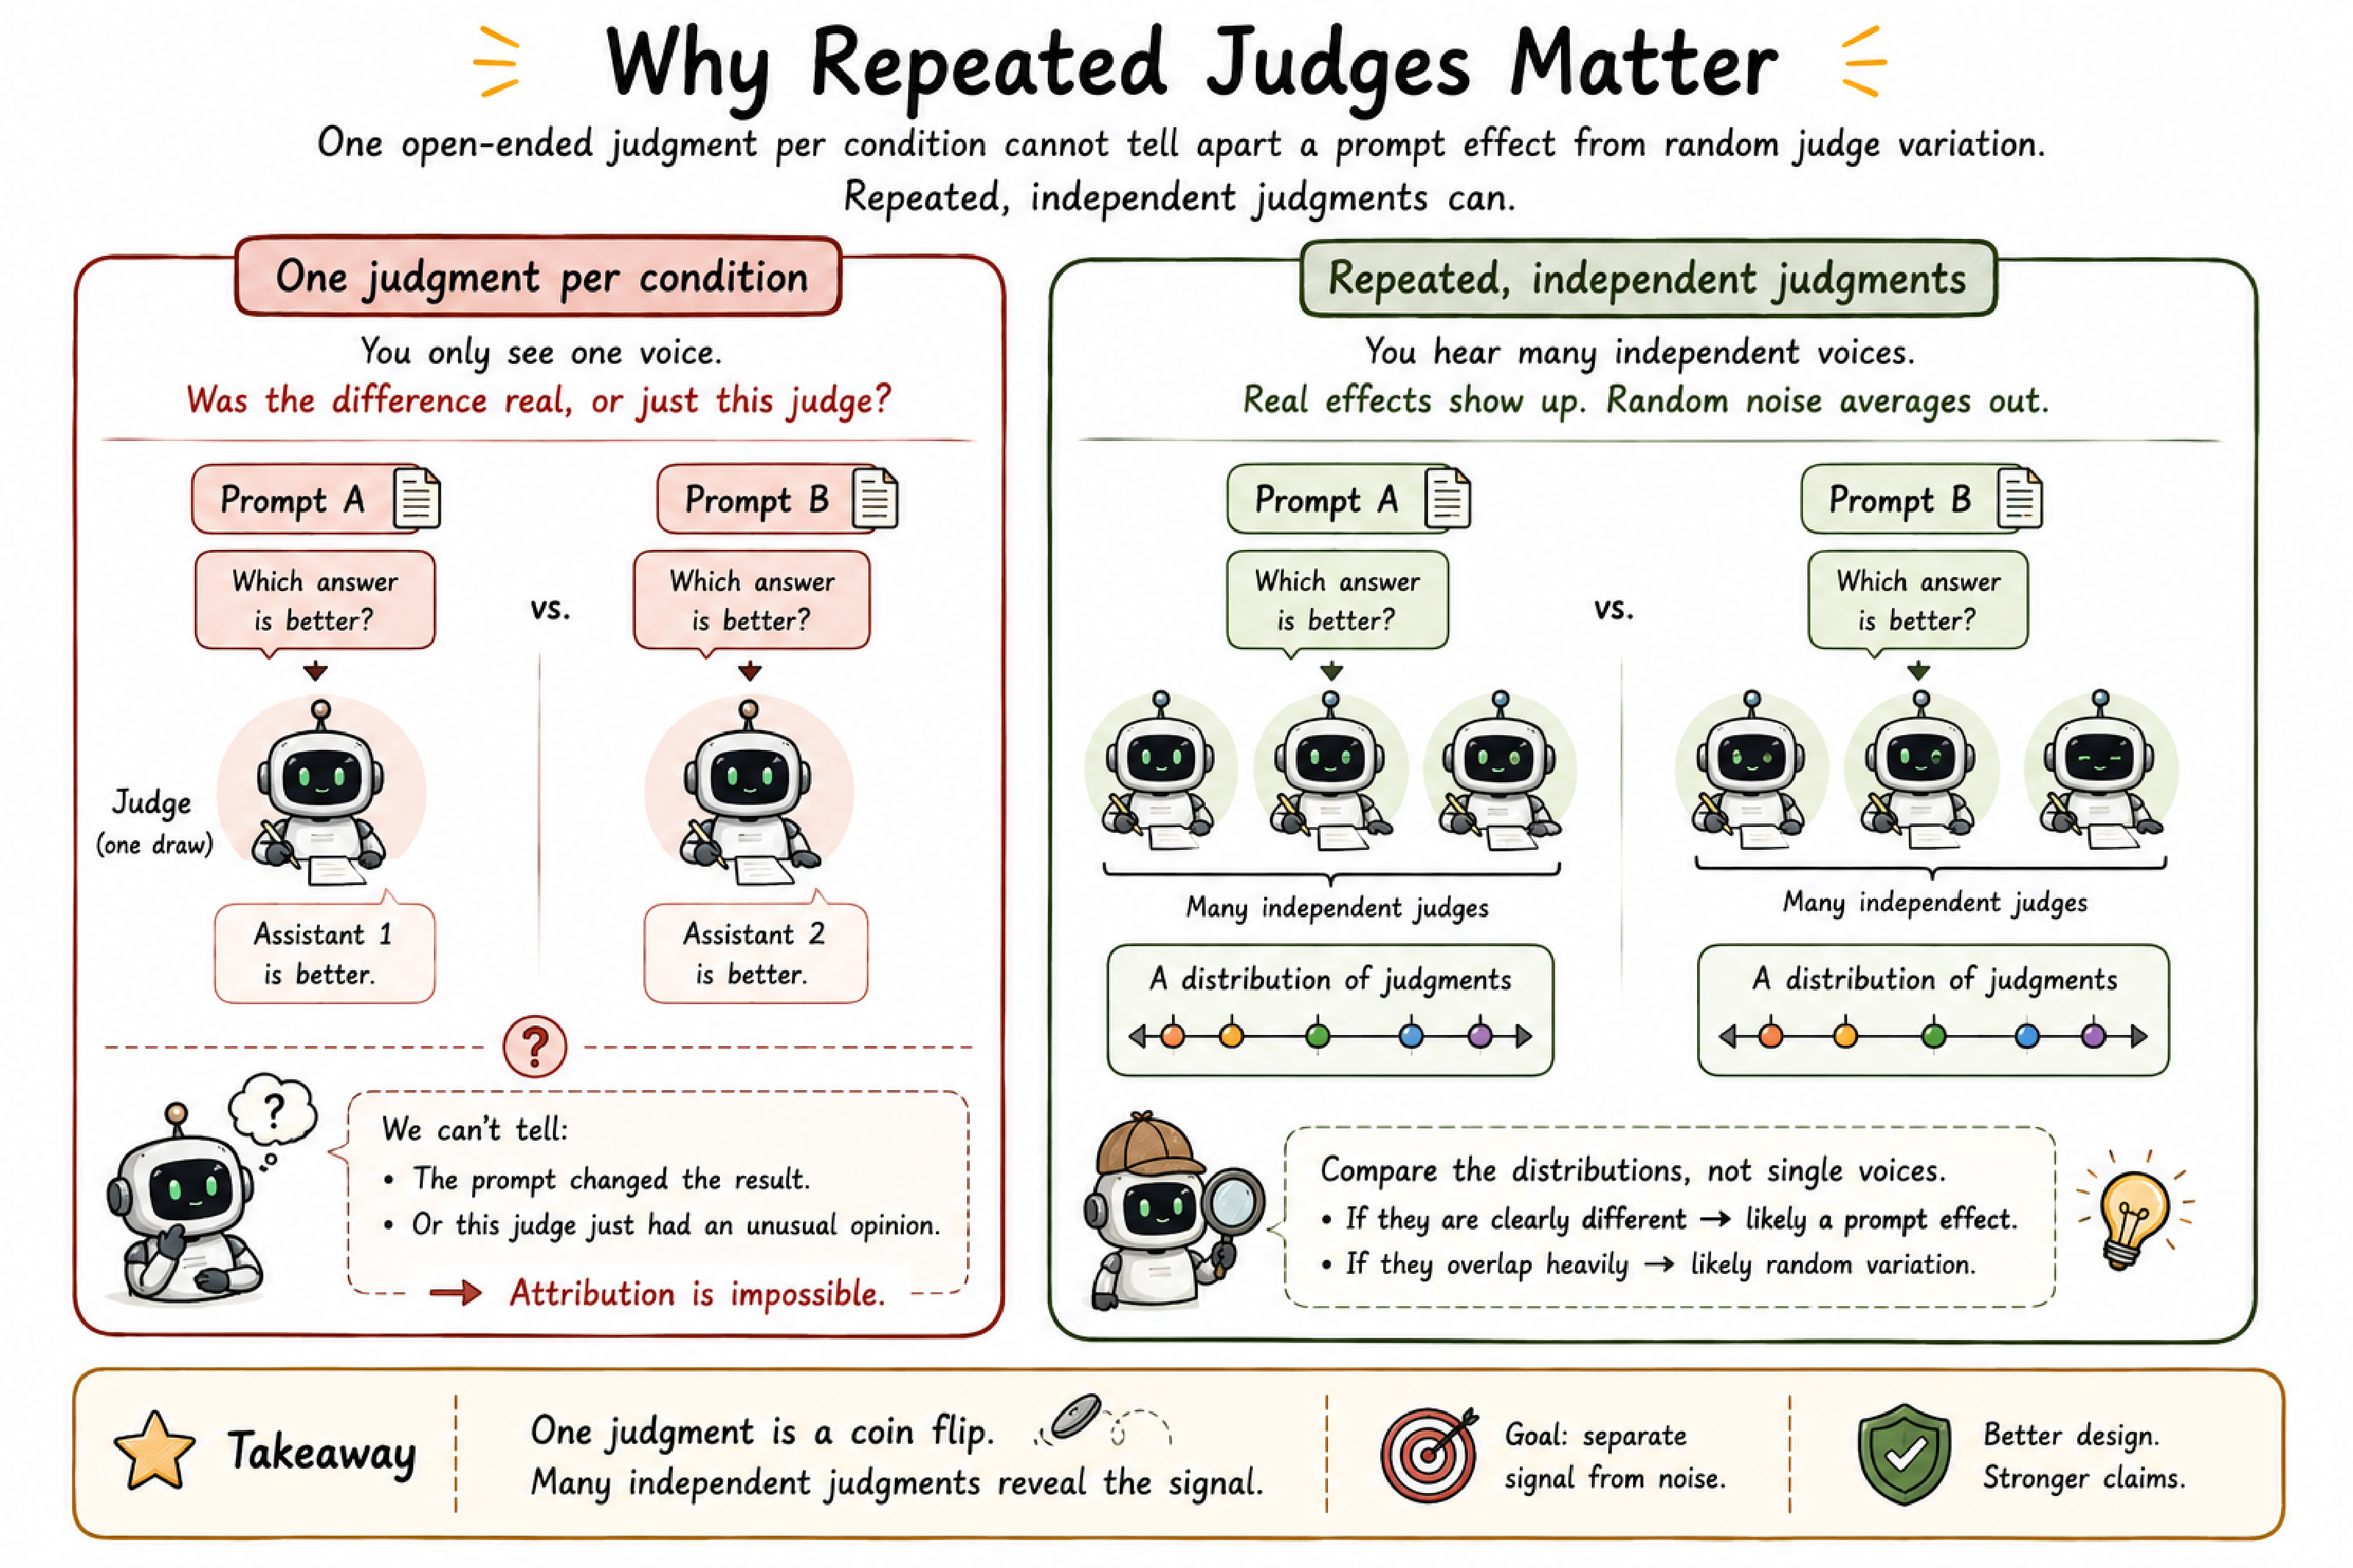
\includegraphics[width=0.98\textwidth]{figures/appendix/repeated_judges.pdf}
\caption*{\small\textit{Conceptual illustration.} Repeated independent judgments matter for open-ended outputs. With
only one judgment per item and condition, a design cannot separately estimate
condition-by-item variation and residual judge variation. Repeated independent
judgments make that decomposition possible, although they do not on their own
establish construct validity or transfer.}
\end{figure*}

The two estimates above use forced-choice probes. This one does not. MT-Bench
\cite{zhengmt2023judging} has models produce free multi-turn text, which a
language-model judge then compares in pairs, and the released judgments record
the same comparison run in \emph{both} presentation orders. Presentation order
is therefore a fully crossed probe factor over an open-ended behaviour. We treat
the item as a (question, model pair, turn) triple and the outcome as the judge's
preference with a tie scored at one half, over $4{,}796$ comparisons on $80$
questions and $30$ model pairs. There is one released judge decision per
item-by-order cell, however, so interaction with order and judge noise are
confounded. This setting identifies the strict main-effect fraction and directly
observed disagreement, but not broad $\phi$.

The result separates two things that are usually reported as one. The
\emph{systematic} part of the position effect is small: the judge prefers
whichever answer it sees first $51.1\%$ of the time, a signed bias of
$\hat\beta=+0.011$ with an item-paired bootstrap interval of
$[+0.006,+0.015]$, small but
reliably non-zero. The \emph{per-item} effect is not small at all. The two
orders disagree on $16.3\%$ of individual comparisons, $8.6\%$ being outright
reversals rather than ties, while $\hat\phi_{\text{strict}}=0.001$. These
quantities make a clear point without overidentifying the decomposition: the
average position effect is small, but a single judged comparison can still be
order-dependent. Repeated, independently sampled judgments per item-by-order cell
would be needed to determine how much of that disagreement is a genuine
item-by-order interaction rather than scorer noise.

That distinction has a practical consequence which cuts \emph{against} the
alarmed reading, and we report it as we found it. Because the bias is
unsystematic, averaging rescues the aggregate: recomputing every model's win
rate under each order separately moves it by at most $10$ percentage points and
reverses only $21$ of $465$ model pairs, or $4.5\%$. A leaderboard built from
these judgments is largely stable. A single comparison from it is not: the two
released orders produce different verdicts on $16.3\%$ of comparisons. The data
cannot separate a genuine order interaction from judge noise. This also explains an
apparent conflict in the literature, where per-comparison flip rates as high as
$82\%$ \cite{wang2024fair} coexist with usable judge leaderboards: the two
numbers concern different aggregation levels and should not be used
interchangeably.

\subsection{Where the Probe Variance Actually Sits}
\label{app:components}

The two-way estimator splits variance into item and probe. That summary hides a
question worth asking: is the probe's effect a \emph{main} effect, a constant
push on every item, or an \emph{interaction}, pushing different items in
different directions? The distinction matters because a main effect is visible
in the mean, whereas an interaction cancels in the mean and is invisible to any
analysis that only asks whether the average moved.

MoralChoice is crossed on three probe factors at once, so we can answer it. We
fit
$y_{ifos}=\mu+a_i+b_f+c_o+(ab)_{if}+(ac)_{io}+(bc)_{fo}
+(abc)_{ifo}+\varepsilon$
over scenario $i$, question form $f$, option order $o$, and sample $s$, and
report each between-cell component as a share of between-cell variation
(Table~\ref{tab:components}).

\begin{table}[t]
\centering
\small
\setlength{\tabcolsep}{4pt}
\renewcommand{\arraystretch}{1.1}
\begin{adjustbox}{max width=\columnwidth}
\begin{tabular}{@{}l r r@{}}
\toprule
\textbf{Component} & \textbf{Dilemmas} & \textbf{Clear answer} \\
\midrule
Scenario (signal)            & $0.514$ & $0.208$ \\
\midrule
Question form                & $0.009$ & $0.212$ \\
Option order                 & $0.062$ & $0.011$ \\
Form $\times$ order          & $0.017$ & $0.037$ \\
\emph{joint-probe main effect} & \emph{0.125} & \emph{0.283} \\
\midrule
Scenario $\times$ form       & $0.189$ & $0.217$ \\
Scenario $\times$ order      & $0.065$ & $0.098$ \\
Scenario $\times$ form $\times$ order & $0.083$ & $0.175$ \\
\emph{item-by-joint-probe interaction} & \emph{0.314} & \emph{0.490} \\
\midrule
Sampling variance (raw)      & $0.120$ & $0.034$ \\
\bottomrule
\end{tabular}
\end{adjustbox}
\caption{Median between-cell sum-of-squares share by component, over $12$
models. Grouped rows are computed within each model before taking the median,
so they need not equal the sum of displayed component medians. The sampling row
is raw within-cell variance, shown separately and not as a share. The probe's
effect is overwhelmingly an interaction with the item rather than a constant
shift: on genuine dilemmas the median within-model ratio is $3.2$, and the
interaction exceeds the main effect for $10$ of $12$ models ($7$ of $12$ on
the clear-answer set).}
\label{tab:components}
\end{table}

Three things follow. First, the interaction dominates: reporting only whether
the \emph{average} moved when the format changed, which is what a main-effect
analysis does, understates probe sensitivity by roughly a factor of three on
this data. This is why we report $\phi_{\text{broad}}$, which counts the
item-by-probe interaction, alongside the narrower $\phi_{\text{strict}}$, and
why the two differ so widely. Second, the two probe factors trade places with
the task, as Appendix~\ref{app:phiempirical} found: form carries $0.212$ where a
clear answer exists and collapses to $0.009$ on dilemmas, where order takes
over. Third, sampling noise is not negligible on dilemmas ($0.120$), so a study
reporting a single generation per item is exposed to a component that more
samples would remove for free. A study that reports one number under one probe
is therefore exposed to all three at once, and cannot tell them apart.

\textbf{Binary and ordinal outcomes.} The decomposition above is on the cell
mean, the reported accuracy or preference rate, which is the level at which the
claim is made, so the components are on the same scale as the number a study
publishes. When one instead wants variance components on the individual binary
responses, the raw proportion mixes the effect of interest with Bernoulli
sampling noise that scales as $p(1-p)$, so a naive components-of-variance on
$0/1$ data attributes structural variance to the residual. The fix is a
generalised linear mixed model: fit
$\text{logit}\,\Pr(y_{ik}=1)=\mu+a_i+b_k+(ab)_{ik}$ with $a_i,b_k,(ab)_{ik}$
Gaussian random effects (a cumulative-link mixed model for ordinal scores), read
the variance components on the latent scale, and take $\phi$ as their probe
share exactly as in Eq.~\ref{eq:phimodel}. On the latent scale the residual is
fixed by the link ($\pi^2/3$ for the logit), so probe variance is not diluted by
sampling noise. We report the cell-mean decomposition in the main text because
it is what a reader reproduces from released outcome tables without refitting a
model; the GLMM is the estimator to prefer when only item-level $0/1$ responses
are available.
For a confirmatory analysis we fit both logit and probit links, inspect
overdispersion and singular random effects, and use posterior-predictive or
parametric-bootstrap checks on the item and probe margins. A conclusion that
changes link function is reported as estimator-sensitive rather than averaged
away.

\subsection{Anchoring the Threshold in a Decision}
\label{app:phithreshold}

An earlier version of this survey proposed $\phi\gtrsim0.5$ as the point at which
a measurement is probe-dominated. That cutoff was intuitive but arbitrary, and
our own data show it is too lenient. We replace it with a threshold derived from
the error a reader will accept.

The reason $\phi$ is decision-relevant is asymmetric shrinkage. Item noise and
sampling noise shrink as a study adds items and samples, which studies routinely
do; a probe effect does not shrink at all unless the study adds \emph{probes}.
In the regime real studies occupy, many items and one probe, the residual share
washes out and the probe share is precisely the error that survives. For two
models truly separated by $\delta$, measured under $K$ probes,
\[
\begin{aligned}
\sigma_{AB}^2&=\sigma_A^2+\sigma_B^2-2\rho\sigma_A\sigma_B,\\
P(\text{inversion})&=\Phi\!\left(-\delta/\sqrt{\sigma_{AB}^2/K}\right),
\end{aligned}
\]
where $\sigma_A^2$ and $\sigma_B^2$ are probe-disturbance variances and $\rho$
is their correlation across probe conditions. Under equal variances,
$\sigma_A^2=\sigma_B^2=\phi\sigma^2_{\rm total}$, the denominator becomes
$\sqrt{2\phi\sigma^2_{\rm total}(1-\rho)/K}$,
which we verified against simulation (agreement to three decimals).

\textbf{Where the expression comes from.} The derivation is three lines and worth
seeing, because it is what makes $\phi$ a design parameter rather than a
descriptive statistic. Write model $A$'s measured score under probe pool $k$ as
its true score plus a probe disturbance, $\hat\mu_A=\mu_A+u_A$, and likewise for
$B$. Averaging over $K$ probes drawn from the pool shrinks that disturbance in
the usual way, so $\mathrm{Var}(u_A)=\sigma^2_{\text{probe}}/K$, and by
definition $\sigma^2_{\text{probe}}=\phi\,\sigma^2_{\text{total}}$. A study
reports the wrong order exactly when the measured difference has the wrong sign,
that is when $(\hat\mu_A-\hat\mu_B)<0$ while the truth is
$\delta=\mu_A-\mu_B>0$. That measured difference is $\delta+(u_A-u_B)$, whose
disturbance term has variance
$(\sigma_A^2+\sigma_B^2-2\rho\sigma_A\sigma_B)/K$. Treating it as approximately
normal and standardising gives the expression above. Independence is therefore
a sensitivity case, not a hidden assumption.
Two features of the result matter more than the algebra. The item count $n$ does
not protect against the common probe main effect in this approximation. An
item-by-probe interaction can average down with more items, so broad $\phi$
requires the fuller design-specific bootstrap. Here $K$ enters only through
$\sqrt{K}$, so
halving inversion risk costs four times the probes, which is why the sizing
question is worth answering before a study is run rather than after.

\textbf{What the bound assumes, and when it fails.} The expression is a normal
approximation and should be read as one. It assumes (i) that the probe effects
entering a model's score are approximately Gaussian once averaged over items,
(ii) that their variance is comparable across the two models being compared
(homoscedasticity), and (iii) that the $K$ probes are drawn independently from
the probe pool a study would actually use. Here $\sigma^2_{\text{total}}$ is the
total variance of the \emph{reported score} on the scale the claim is made,
pooled over items within a model, and $\delta$ is the true difference between two
models' scores on that same scale; both are therefore metric-specific, and the
threshold must be recomputed when the reported quantity changes. Assumption (i)
is the one that bites. It is reasonable when a score averages many items, by the
central limit theorem, and unreliable in three regimes: very small probe pools
($K\le3$, where the average of a handful of probe effects is not yet normal),
scores near a floor or ceiling (where the binomial variance $p(1-p)$ makes the
effect heteroscedastic and the distribution skewed), and heavy-tailed probe
effects, which arise when one pathological format dominates the pool. In all
three, the closed form understates risk on the skewed side. The remedy is
cheap and needs no new data: resample probes with replacement and read the
inversion rate off the bootstrap directly, which is what
Appendix~\ref{app:phici} compares against the closed form. On our data the normal
approximation is accurate on the dilemmas ($0.290$ against a bootstrap $0.275$,
Spearman rank correlation $0.90$) and conservative on the low-ambiguity set ($0.288$ against
$0.186$), exactly the ceiling regime the assumption predicts. We therefore do
not offer a universal $\phi$ cutoff. A numerical threshold additionally requires
the score scale, the pairwise gap, the model correlation, and the admissible probe
population. Table~\ref{tab:ktable} is a conditional sensitivity illustration,
not a data-derived pass/fail rule; a named ranking should instead report its
paired probe-bootstrap inversion rate.

The measured correlation is positive rather than zero: median $\rho=0.435$ on
dilemmas and $0.800$ on clear-answer items, with $53/66$ and $58/66$ model pairs
positive. Under equal variances the independence table is conservative by
$1/(1-\rho)$, factors $1.77$ and $4.99$ at those medians. For a named model pair
we therefore bypass the equal-variance approximation and paired-bootstrap the
difference. On dilemmas, five of the other eleven models are more
probe-dependent than GPT-4 at the $97.5\%$ paired-bootstrap level. One model is
significantly less probe-dependent, so the broader claim that GPT-4 is the most
robust does not survive. No such comparison survives on the clear-answer set.

The predicted failure rate is borne out. Across the six probe conditions,
$76\%$ of the $66$ model pairs reverse their ordering on the high-ambiguity set
and $44\%$ on the low-ambiguity set. Among pairs separated by less than five
percentage points, \emph{every} pair reverses; below ten points, $94\%$ do.
Three different models can be named the most moral of the twelve depending on
which question form and option order the study happened to use. A leaderboard of
moral behaviour built from a single probe is, at these effect sizes, close to
arbitrary.

\subsection{What Each Remedy Buys}
\label{app:mitigation}

A remedy recommended without a measured effect is just another assertion, so we
measure what each one buys. The crossed MoralChoice design lets us simulate
each remedy by aggregating over the probe factor it would have controlled, and
then ask what a study using that protocol would still be exposed to. We report
the residual probe variance of a model's score and, more directly, the
\emph{verdict-flip rate}: how often two models' ordering reverses between two
independent applications of the same protocol.

On the genuine dilemmas, a single probe leaves a probe variance of $0.025$ and
flips $36\%$ of pairwise verdicts. Symmetrising the two option orders within one
question form costs twice the inference and cuts those to $0.003$ and $16\%$, a
removal of $88\%$ of the variance and $55\%$ of the flips. A template ensemble
over the three question forms costs three times the inference and removes only
$29\%$ and $22\%$. On the clear-answer items the ranking of remedies reverses:
template ensembles remove $75\%$ of the variance against order symmetrisation's
$25\%$.

\textbf{Reading these as $\phi$ before and after.} A mitigation acts on the
\emph{numerator} of $\phi$, the probe variance, while leaving the signal it is
measured against unchanged; the percentages above are therefore exactly the
before-and-after change in that numerator, and the flip rates are its
decision-level consequence. We deliberately do not report $\phi$ itself as a
ratio after a mitigation, because averaging over a probe factor removes variance
from the denominator as well, so the residual shares mechanically inflate and a
successful remedy can appear to raise $\phi$. The quantity to compare across
remedies is the absolute probe variance (or the flip rate), with $\phi$ read once
on the unmitigated design to decide whether a remedy is worth testing. The
acceptable residual depends on the score scale, model gap, probe population, and
accepted reversal risk; this table identifies the largest reduction in this
specific design rather than a universal requirement.

\subsection{How $\phi$ Relates to Other Sensitivity Indices}
\label{app:phivsposix}

Several indices now summarise probe sensitivity, and a reader is entitled to ask
whether $\phi$ is a fourth name for the same thing. Conceptually the measures
differ in what they attach to. POSIX \citep{chatterjee2024posix} scores how far a
\emph{model's output distribution} moves under perturbation, so it is a property
of a model. $\Pi_m$ \citep{romanou2026brittlebench} partitions benchmark variance
and is a property of a benchmark-model pair. $\phi$ is the share of a
\emph{reported measurement} that is probe rather than signal, so it is a property
of a claim: the same model can have a low $\phi$ for one claim and a high $\phi$
for another measured on the same outputs, because the denominator changes with
what the study says it is measuring. Related proposals estimate how many prompt
resamplings a reliable estimate needs \citep{lior2025reliableeval} or score the
worst prompt rather than the average \citep{cao2024worst}; these answer design
and lower-bound questions rather than the attribution question.

Generalizability-theory and many-facet rater models are complementary rather
than competing estimators. They model declared facets, such as raters, tasks,
and formats, then use a D-study to allocate a future measurement budget. IRT is
the right tool when item difficulty and a latent ability scale are the target.
$\phi$ is the smaller, claim-relative report one can compute after that design:
the observed share assigned to one named probe axis. It does not establish
construct validity by itself.

Empirically they agree about which models are fragile. On the MoralChoice
dilemmas we computed, for each of the $12$ models, $\phi_{\text{broad}}$ and a
POSIX-style index defined as the mean over scenarios of the spread of
$P(\text{action 1})$ across the six probe conditions. The two rank models almost
identically (Spearman $\rho=0.92$, $p<0.001$; Pearson $r=0.95$). This is the
expected result and it is reassuring rather than redundant: when the signal is
held fixed, as it is within one corpus, a model whose outputs move more under
perturbation also has a larger probe share. The indices come apart precisely when
the signal changes. A capability benchmark and a behavioural probe can produce
similar output spreads while their $\phi$ values differ by two orders of
magnitude, because the between-item signal is large in the first case and small
in the second; this is the contrast in Appendix~\ref{app:phiempirical}, and it is
invisible to an index that does not divide by the signal. The practical rule is
that a model-attached index answers ``is this model twitchy'', whereas $\phi$
answers ``does this particular reported number survive'', and only the second is
what a validity audit needs.

That reversal is not a curiosity, it follows from the variance components of
Appendix~\ref{app:phiempirical}. Where a clear answer exists the format
term dominates, so averaging formats is the effective remedy; on genuine
dilemmas the order term dominates, so symmetrising orders is. The general rule
is therefore cheap and specific: estimate the components first, then spend the
inference budget on the factor that carries the most variance, rather than
applying a favoured remedy by habit. Two caveats. Averaging all six conditions
drives the measured residual to zero by construction, since no probe variation
remains \emph{within this design}; paraphrase, persona, and seed variation are
untouched by it and would reappear in a wider pool. And these are efficacies for
one behavioural task, so they justify the decompose-then-target rule rather than
the specific percentages.

\subsection{Confidence Intervals and the Normal Approximation}
\label{app:phici}

A severity index reported without an uncertainty analysis invites the same single-number
habit this survey argues against. Our earlier items-only bootstrap was wrong for
a claim about a finite probe pool: it conditioned on the six conditions and
therefore omitted the larger source of uncertainty. Resampling scenarios and
probe conditions together changes the median strict-$\phi$ sensitivity width from
$0.034$ to $0.172$ on dilemmas and from $0.062$ to $0.382$ on clear-answer
items, inflation factors $5.1$ and $6.2$. For broad $\phi$, the dilemma width
changes from $0.046$ to $0.303$. Only $3/66$ dilemma pairs and $7/66$
clear-answer pairs have non-overlapping sensitivity intervals. These resamples
treat the six compound form-by-order cells as a finite probe pool; they are not
population confidence intervals over all possible wordings and orders. The ordering of
models by point-estimate fragility is not well separated; only a paired
bootstrap can support a named comparison.

The normal approximation is adequate where it is used and degrades where it is
not. Comparing its predicted inversion rate against the rate measured directly
by drawing probe conditions, the mean predicted and empirical rates agree
closely on the high-ambiguity set ($0.290$ against $0.275$, median absolute
discrepancy $0.022$, rank correlation $0.90$). On the low-ambiguity set the
approximation is conservative, over-predicting inversions ($0.288$ against
$0.186$), because the per-condition scores there are strongly skewed rather than
symmetric. The practical recommendation follows: use the closed form for design
and sizing, where being conservative is the right error, and report the
bootstrap rate when making a claim about a specific pair.

\begin{table}[t]
\centering
\small
\setlength{\tabcolsep}{4pt}
\renewcommand{\arraystretch}{1.12}
\begin{adjustbox}{max width=\columnwidth}
\begin{tabular}{@{}l r r r@{}}
\toprule
& \multicolumn{3}{c}{\textbf{probe variants $K$ needed}} \\
\cmidrule(l){2-4}
\textbf{fragility $\phi$} & small gap & typical gap & large gap \\
\midrule
$0.05$ & $8$   & $2$  & $1$ \\
$0.10$ & $16$  & $4$  & $1$ \\
$0.25$ & $40$  & $8$  & $3$ \\
$0.50$ & $80$  & $16$ & $5$ \\
$0.75$ & $120$ & $24$ & $8$ \\
\bottomrule
\end{tabular}
\end{adjustbox}
\caption{Conditional MoralChoice-scale illustration: probe variants needed under a
normal, equal-variance approximation to hold inversion risk below $5\%$. The
rows assume a common score scale and probe population, and the columns use the
$25$th percentile, median, and $75$th percentile gaps observed on MoralChoice
($0.041$, $0.095$, $0.167$). Total score variance is anchored at twice the
observed mean probe variance, equivalently $\phi=0.5$ at that anchor. The table
is not a universal $\phi$ threshold: a
new study must supply its own score scale, model correlation, and bootstrap
check.}
\label{tab:ktable}
\end{table}

\subsection{Does Contamination Change the Spread, Not Just the Level?}
\label{app:contam}

We argue in Appendix~\ref{app:t6mech} that memorisation moves a score's level
rather than its spread, so a variance ratio should survive it. That deserved a
test rather than an assertion, and testing it turned up a real counterexample,
which we report because it revises one of our own numbers downward.

The mechanism is arithmetic. A binary outcome with mean $p$ has variance exactly
$p(1-p)$: for $0/1$ data the spread is fixed by the level. An item the model has
memorised is answered correctly under every phrasing, so $p$ approaches $1$ and
its probe variance approaches zero, not because the probe stopped mattering but
because there is no room left to move. Contamination, by raising $p$, compresses
probe variance as a side effect.

The size of the effect is what matters, and on a heavily exposed benchmark it is
large. Re-analysing PromptEval, which records $0/1$ correctness for MMLU items
under $100$ meaning-preserving templates \citep{polo2024efficient}, we find that
a median of $37\%$ of items sit at a ceiling ($p\ge0.9$) and $41\%$ at a floor
($p\le0.1$), so roughly four items in five carry almost no room for a probe
effect. Computing $\phi_{\text{strict}}$ over all items gives a median of
$0.001$; computing it over only the mid-difficulty items ($0.2<p<0.8$) gives
$0.033$, about twenty times larger, and the direction is the same in $47$ of the
$47$ subject-model matrices we examined. The more ceiling items a matrix
contains, the larger the correction (Spearman $\rho=0.47$).

Two consequences follow. First, our headline capability figure of $\phi\approx
0.003$ is deflated by this mechanism, so the honest comparison against the
behavioural corpus is roughly one order of magnitude rather than two. The
qualitative claim, that the tested dilemma axis has larger strict $\phi$ than
the matched MMLU template axis, survives; the multiplier does not. Second, this
ceiling mechanism has a known sign: it pushes $\phi$ down and can make a fragile
finding look robust. A study reporting a small $\phi$ on a
benchmark whose items cluster at the ceiling should say so, or restrict the
estimate to mid-difficulty items, which costs nothing but a filter.

\subsection{Does the Interaction Ever Change the Verdict?}
\label{app:verdictflip}

Including the item-by-probe interaction raises $\phi$, but a reviewer is right to
ask whether it ever changes a \emph{decision} rather than a number. It does, and
routinely.

Take the design rule above: a study running $K=5$ probe
variants that will accept a one-in-twenty chance of ranking two models the wrong
way round. Its budget is $\phi\le0.17$. Reading the same MoralChoice data both
ways, eight of the twelve models pass on the additive reading and fail once the
interaction is counted. On the clear-answer items the same design reverses five
of twelve at $K=5$. A study using the additive model would have declared its probe pool
adequate and published a ranking that its own data does not support.

\subsection{Does the Probe Story Hold Outside These Two Corpora?}
\label{app:crossbench}

The empirical base for $\phi$ is narrow, and the fair question is whether the
pattern is a quirk of the corpora we happened to re-analyse. We can give a
partial answer from an independent source. A pre-existing companion run applies the
same crossed logic, one frozen model answering each item under a panel of
persona, paraphrase and option-order views, across twelve benchmarks and four
open-weight models, and stores a variance decomposition per cell. Several of its
benchmarks are cultural or cross-national rather than English forced choice:
NormAd etiquette norms asked plain, by country, by value and by both,
GlobalOpinionQA, DICES, and D3CODE.

One caveat governs how far we can read it. That run stored the components
\emph{within} each item and averaged over items, and did not retain the
between-item term, so it gives the composition of $\phi$'s numerator, what the
probe contributes and how it splits, but not $\phi$ itself, which needs the
signal in the denominator. We report it as such.

Read that way it replicates the finding that surprised us most. Across the $48$
benchmark-by-model cells, option order carries a median $69\%$ of the probe
variance and is the largest of the three axes in $33$ of them, with persona at
$20\%$ and paraphrase at $4\%$. On the cultural and cross-national benchmarks
specifically, order carries $73\%$. The probe term is about five times the
within-item residual. It is not universal, and the exceptions are informative in
the same way the main-text contrast is: on D3CODE and Scruples paraphrase
dominates instead, and on MoralBench persona takes almost all of it. Which axis
matters is a property of the task, which is exactly why we recommend decomposing
before choosing a remedy rather than reaching for a default.

\subsection{A Different Variance Decomposition}
\label{app:altdecomp}

One further clarification pre-empts a natural confusion. Variance decomposition
has been applied to language model behaviour before, but at the level of
next-token probability over pretraining: \citet{michaelov2025phases} explain up
to $98\%$ of word-level variance with frequency, $n$-gram, and semantic
similarity heuristics. Our estimand is different. The fragility fraction is the
share of variance in a \emph{behavioural measurement} attributable to the
\emph{probe}, with the model held fixed.

\subsection{Why We Do Not Pool the Corpora}
\label{app:pooled}

A catalogue of existence proofs is not a pooled magnitude, but neither is a
meta-analysis obtained by treating models sharing one finite probe pool as
independent studies. That shortcut conditions on the probes, recreates the
items-only interval error of Appendix~\ref{app:phici}, and invites pooling
claim-relative quantities measured on different axes. We therefore withdraw the
earlier DerSimonian-Laird pooled values and use the harmonised table only for the
specific comparison between MMLU and MoralChoice that it identifies.

A reliable pooled estimate per threat requires primary studies to release
probe-level outcomes, a common estimand and task-family pool, and uncertainty
that propagates item, probe, and study sampling. The present literature rarely
provides the first of these. The living repository therefore stores per-effect
records and subset curves, not a domain constant. Heterogeneity across models and
axes remains a result; averaging it into one number would erase the result.

\subsection{When Judge-Based Scoring Helps, and When It Hides}
\label{app:judgescoring}

A natural objection to the reliability tier is that some of the sensitivity it
documents is an artefact of \emph{scoring} rather than of the model, and that
replacing brittle exact-match scoring with a model judge reduces measured
prompt variance. Both halves of that claim can be true at once, and the
distinction that matters is where the variance went.

Two mechanisms produce a drop in $\phi$ after switching to a judge, and they
have opposite implications. In the first, the original variance was \emph{scoring error}: the model's behaviour was stable but a string matcher failed on valid paraphrases, so a semantic scorer removes measurement noise that was never in the model. \citet{hua2025flaw} make exactly this case, finding across seven models and six benchmarks that much reported prompt sensitivity traces to heuristic scoring rather than to the model. This is a genuine improvement and exactly what the
reliability tier asks for. In the second, the variance was real behavioural
instability, and the judge absorbs it by imposing its own prior, so the reported
number stabilises because it now reflects the judge rather than the subject.
Position, verbosity, and self-enhancement priors are documented in judges at
scale \cite{ye2024justice,wang2024fair,zhou2026judgebias}, and a length-controlled
protocol raises agreement with humans from $0.94$ to $0.98$ precisely because
uncontrolled verbosity was doing part of the scoring
\cite{dubois2024lengthcontrolled}. A stabilised number from an unaudited judge
is a T1 improvement bought with a T3 liability.

The two are separable with tests this survey already recommends. First, audit
the judge as an instrument in its own right: report its signed position-bias
statistic with an interval and its self-agreement across meaning-preserving
rephrasings \cite{bellibatlu2026judgesense}, so that any variance the judge
removes can be compared against variance the judge itself contributes. Second,
apply the behavioural-entailment condition of
Appendix~\ref{app:construct}: check that the judge-scored quantity still
predicts held-out behaviour it was not fitted to. A judge that lowers $\phi$
while preserving entailment has removed scoring error; a judge that lowers
$\phi$ while entailment degrades has replaced a noisy measurement of the model
with a quiet measurement of the judge. Reporting $\phi$ alone cannot tell these
apart, which is why the index is proposed as one tier of an audit rather than as
a summary statistic.

\section{A Worked Audit End to End}
\label{app:casestudy}

\textbf{The audit end to end.} Applied to the claim that a model \emph{has} a
stable personality profile, all three tiers fail in sequence: equivalent prompts
yield significantly different Big Five scores \cite{gupta2024self,shu2024dont};
up to $90\%$ of between-model variance is response bias rather than trait
\cite{meyer2026apparent}; and the questionnaire barely predicts open-ended
behaviour \cite{song2025psychometric}. What began as ``model $M$ has personality
$X$'' is, audited, a statement about the questionnaire
\cite{suhr2023challenging}. Not every claim fails, and it matters that the
framework says so: judge \emph{position bias} passes all three tiers, and our own
analysis adds a narrower second survivor on the genuine dilemmas: five named
models are more probe-dependent than GPT-4 in a paired bootstrap over all six
conditions
\cite{shi2025judging,wang2024fair,li2025calibraeval}. At high
fragility the supported claims are about stability under probe variation, not
the level of a disposition (Appendix~\ref{app:casestudy}).

Section~\ref{sec:checklist} audits a personality claim; we run a second claim,
that \emph{language models are cooperative}, through the same three tiers, and
close with a claim that survives. \textbf{Reliability.} Measured cooperation is
probe-dependent: decoding and format move it (Section~\ref{sec:reliability}),
and its value is not read off a single prompt. \textbf{Validity.} The construct
and comparison target are unstable: cooperation falls from $95\%$ to $16\%$
between a model and its reasoning-tuned variant \cite{li2025spontaneous}, while
framing and payoff structure both alter strategic behaviour, with their relative
importance varying by model \cite{lore2024strategic}. Thus ``cooperative''
conflates a disposition, model configuration, and test design.
\textbf{Generalizability.} The canonical
Prisoner's Dilemma is the easy, probably memorised case; welfare swings from
$7\%$ to $80\%$ once payoffs are rewritten \cite{tewolde2026coopeval}, and
societies of the same agents fail to sustain a shared resource in more than
half of runs \cite{piatti2024govsim}. ``Language models are cooperative''
survives no tier as stated; what survives is the narrower, probe-indexed claim
that a \emph{specific} model cooperates at a measured rate in a \emph{specific}
game under a \emph{stated} payoff and framing.

\subsection{A Named Re-Audit, and What It Changes}
\label{app:reaudit}

The audits above are constructed from magnitudes reported across many papers. It is fair to ask for one worked end to end on a single published study, with
its own data, so that the change in conclusion is visible rather than argued. We use \citet{scherrer2023evaluating}, and we chose it precisely because
it is careful work: the authors cross three question forms with both option
orders and five samples, release every response, and state plainly that their
low-ambiguity and high-ambiguity sets support different kinds of claim. It is
because they did all of that that a re-audit is possible at all; a study
reporting one number under one probe could not be audited by anyone, including
its authors. Nothing below contradicts a claim they make. What it shows is which
readings their data licenses, which is a question the field has not had the
vocabulary to ask.

\emph{Reliability.} Recomputing the fragility fraction on their released
responses gives a median $\hat\phi_{\text{broad}}$ of $0.38$ on the genuine
dilemmas, with two of twelve models above $0.5$, and a measured preference that
moves by up to $94$ percentage points across the six probe conditions
(Appendix~\ref{app:phiempirical}). A per-model rate of moral choice, read from
any single question form and option order, is therefore not reproducible at the
precision at which such rates are usually quoted.

\emph{Validity and generalizability.} The consequence for comparison is sharper
than for any single model. Across the six conditions, $76\%$ of the $66$ model
pairs reverse their ordering; among pairs separated by less than five percentage
points, every pair reverses; and three different models can be named the most
moral of the twelve depending only on which form and order a study happened to
use (Appendix~\ref{app:phithreshold}). A ranking of models by moral behaviour
built from a single probe is, at these effect sizes, close to arbitrary.

\emph{What survives.} The re-audit is not a demolition, and this is the part we
would emphasise. The scenario \emph{profile} replicates strongly across probe
conditions (split-half rank correlation $0.89$ after correction) and is
more stable across tested probes than across models
(Appendix~\ref{app:structural}). So the relational claim, that a given model
finds these scenarios harder than those, is well supported by exactly the data
that does not support the absolute claim. The conclusion changes from ``model
$M$ chooses the moral action $x\%$ of the time, and more often than model $N$''
to ``model $M$ orders these dilemmas in this stable way''. That is a narrower
claim, but it is one the measurement earns, and it is the template we would like
future studies to reach for.

\subsection{A Claim That Survives}
\label{app:survivor}

The framework credits robust findings, not only
debunks fragile ones. That judges carry a \emph{position bias} is itself a
reliable, valid, and general claim: it reproduces across runs with test-retest
stability typically above $0.95$ (reported range $0.93$ to $1.00$)
\cite{shi2025judging}, it is measured by a construct
(order sensitivity) that the instrument directly manipulates rather than
borrows from humans, and it transfers across datasets and judge families
\cite{wang2024fair,li2025calibraeval}. A claim reported as a function of the
probe, with its fragility quantified, is exactly what the checklist is meant to
let through.

A second survivor comes from our own estimates, and it is instructive because it
is \emph{comparative} rather than a stable-trait claim. On the moral-dilemma data of
Appendix~\ref{app:phiempirical}, almost no absolute claim survives: preferences
move by up to $94$ points across probe conditions and $76\%$ of model pairs
reverse their ordering. But a narrower comparative claim does on the genuine
dilemmas. GPT-4 has $\hat\phi_{\text{broad}}=0.20$ on the common panel. Five of
the other eleven models have larger values at the $97.5\%$
paired-bootstrap level. One model is significantly lower, so the data do not
support calling GPT-4 the most robust. No such comparison survives on the
clear-answer set. The surviving claim must therefore name both the comparison
set and probe pool.

\section{Threat-Specific Protocols and Templates}
\label{app:t6mech}

This appendix collects the operational recipes referenced from the body, one per
threat: the ecological mechanisms of T6 and a leakage protocol, the scoring-target
discipline for T4, the instrument redesign for T3, and an auditing recipe beyond
English and text. Each is a procedure a study can run, not a caveat it can state.

\textbf{Ecological mechanisms (T6).} A further interaction belongs here.
T4$\times$T6 runs through contamination: a canonical benchmark is both the
likeliest to be memorised and the likeliest to have a settled scoring target, so
a model can look correct against the scoring standard exactly where the answer is
recalled rather than computed, and the two threats mask each other. T6 otherwise
aggregates distinct failure mechanisms that share a probe-to-deployment gap but
call for different safeguards (Table~\ref{tab:t6mech}). Separating them lets a
study report residual risk per mechanism rather than a single caveat.

\begin{table}[H]
\centering
\footnotesize
\setlength{\tabcolsep}{3pt}
\renewcommand{\arraystretch}{1.18}
\begin{adjustbox}{max width=\columnwidth}
\begin{tabular}{@{}>{\raggedright\arraybackslash}p{1.9cm}>{\raggedright\arraybackslash}p{2.6cm}>{\raggedright\arraybackslash}p{2.5cm}@{}}
\toprule
\textbf{Mechanism} & \textbf{Diagnostic} & \textbf{Safeguard} \\
\midrule
Transfer failure & Information-asymmetric, multi-turn variant \cite{liu2024autonomous} & Report the toy-to-deployment gap, not the toy score \\
Contamination / leakage & Canonical-vs-novel and payoff-perturbed gap \cite{tewolde2026coopeval,sainz2023nlp} & Procedurally generated items; a contamination registry \\
Eval-awareness & Deployment-vs-eval discrimination test \cite{needham2025evalaware} & Held-out task families; blinded, deployment-like probes \\
Sandbagging & Capability elicitation under incentive \cite{vanderweij2025sandbagging} & Adversarial elicitation; report the elicited ceiling \\
Emergent dynamics & Multi-agent run absent from single probes \cite{park2023generative,ashery2025emergent} & Report population-level effects separately from individual ones \\
\bottomrule
\end{tabular}
\end{adjustbox}
\caption{The five mechanisms folded into T6, each with a distinct diagnostic and
safeguard. A behavioural study touching deployment should state which mechanisms
it controlled for and the residual risk from those it did not.}
\label{tab:t6mech}
\end{table}

\subsection{A Leakage and Calibration Protocol}
\label{app:leakcal}

Two operations in the table need more than a pointer.

\textbf{Leakage.} Use a matched canonical-to-novel design. For each canonical
item, such as a named game or published questionnaire, create a semantically
matched novel version by procedural generation or payoff perturbation. Hold the
remaining features fixed. Report the canonical-minus-novel gap as the leakage
estimate, rather than reporting the canonical score alone. A non-zero gap bounds
how much of the headline result may be recall.

Screening item text against a contamination registry \cite{sainz2023nlp} is a
useful first pass, but it cannot detect paraphrased memorisation. When the
canonical-to-novel gap is ambiguous, add one of two controls. Provenance
filtering keeps items first made public after the model's training cutoff.
Dynamic generation draws a fresh item family for each evaluation from an
evaluator-controlled generator. The trade-off should be explicit: provenance
filtering reduces and recentres the item pool; dynamic generation prevents exact
memorisation but requires a versioned, released generator for comparisons across
evaluations.

\textbf{Calibration.} A model-based judge or annotator needs a jointly labelled
shared set $D_{\text{shared}}$. Draw it from the target distribution and stratify
it over every subgroup named in the claim. Label it with the gold procedure the
judge is intended to replace, and keep it separate from all data used to select
or tune that judge. Set its size by the desired precision, power, subgroup
coverage, and sampling design rather than by a generic item count.
Prediction-powered inference is one construction that combines those labels
with model predictions and provides an interval under its stated assumptions
\cite{angelopoulos2023ppi}.

\subsection{Choosing and Reporting a Scoring Target (T4)}
\label{app:scoringtarget}

Normative-benchmark
validity fails silently when the scoring standard is left implicit, so we recommend
stating it as an explicit choice among three, in this order. If the claim is
about \emph{optimality}, score against the game-theoretic solution and report
the solution concept used. If the claim is about \emph{preference}, do not score
against equilibrium at all: infer the implied objective from choices by revealed
preference and report that objective, which separates ``incoherent'' from
``coherently optimising something else''. If the claim is about
\emph{human-likeness}, score against a stated human reference population, and
report which one, since the same behaviour can be human-like against one
population and not another. Divergence across the three is itself a result and
should be reported: a model that is far from equilibrium, coherent under
revealed preference, and close to a human sample is not irrational but is
optimising a human-like objective, and the three targets should not be
collapsed into one verdict.

\subsection{A Reporting Template for the Scoring Target}
\label{app:t4template}

The procedure above says which target to choose; this says what to print. A T4
report should carry five fields, and the discipline is that the first three are
fixed \emph{before} the results are seen.

\textbf{Target.} The scoring rule, named: a solution concept (which one),
a revealed-preference objective (over what choice set), or a human reference
population (which sample). \textbf{Justification.} One sentence on why that
target answers the question asked, since ``irrational'' is only meaningful
relative to a stated optimum. \textbf{Alternatives.} The other targets that were
plausible and will also be scored. \textbf{Divergence.} The score under each
target, with intervals, reported side by side rather than collapsed.
\textbf{Verdict.} A statement in the form licensed by the pattern: agreement
across targets supports ``the model is (in)coherent''; disagreement supports
only ``the model is far from target~A while coherent under target~B'', which is
a claim about the objective and not about the model's competence. A model that
is far from equilibrium, coherent under revealed preference, and close to a human
sample is not irrational, and a report that prints only the first number will say
that it is.

\subsection{Instrument Redesign for T3: Response Style and Forced Choice}
\label{app:sdr}

The construct tier has a mitigation literature the survey should name, because
it addresses the exact failure that Appendix~\ref{app:catalogue} records as the
largest single artefact. When $81$ to $90\%$ of between-model variance on
personality batteries is directional response bias rather than trait
\cite{meyer2026apparent}, the diagnosis is a response-style problem, and the
psychometric remedy is instrument redesign rather than post-hoc correction.
Two moves transfer to models. \emph{Graded forced choice} replaces a rating
scale with a choice between statements matched on desirability, which removes
the shared direction that acquiescence and desirability exploit; the cost is that
raw scores become ipsative, comparable within a subject but not across subjects,
so between-model comparison then requires a normative model fitted at the item
level rather than raw sums. \emph{Desirability matching} requires items paired on
an independently measured desirability rating, which for models must be measured
on models rather than borrowed from human norms, since desirability is exactly
the property least likely to transfer. Both are testable within the criterion of
Appendix~\ref{app:construct}: a redesigned instrument should raise structural
replication and lower the artefact share without collapsing the trait signal,
and a redesign that lowers artefact variance while also destroying behavioural
entailment has removed the construct along with the bias.

\subsection{Auditing Beyond English and Text}
\label{app:mmrecipe}

Section~\ref{sec:mmul} argues the threats recur across languages and modalities;
the checklist needs a concrete form there. The probe pool acquires one axis per
channel. For \emph{multilingual} audits, the pool should cross at least the
formats and orders already required with a language set chosen for typological
and resource spread rather than convenience, and the reported statistic should be
per-language rather than pooled, since a pooled mean hides exactly the
low-resource collapse the audit is looking for. Cross-language self-agreement is
the natural reliability statistic, but it must be reported against a stated
item set: a $\kappa$ computed over easy items is not comparable to one computed
over hard items, so we recommend reporting $\kappa$ alongside the per-language
accuracy it was computed at. For \emph{multimodal} audits the perturbation set is
modality-specific and must preserve meaning in that modality: for images,
crops, resamplings, and small spatial shifts; for audio, speaker, speed, and
noise variation; for both, the option-order permutations that text audits already
use, since order priors are not text-specific
\cite{atabuzzaman2025mcqa,lin2025hearing,rosenfeld2025questioning}. The
fragility fraction is defined identically in each case. Its unitless form permits
a common report, but not unrestricted numerical comparison: comparisons require
compatible outcome links, item populations, ceiling regimes, and declared probe
universes. A study should therefore report $\phi$ per language or modality before
comparing them, rather than pooling incomparable perturbations.

\section{Toward a Model-Native Criterion for Constructs}
\label{app:construct}

The framework this survey imports was built for people, and the objection that a
language model is not a person is fair. We therefore propose a minimum
\emph{behavioural evidence bundle} for a construct claim, in terms that never
ask whether the model resembles a human. The three checks below can support a
probe-indexed interpretation of $X$ for model $M$; they are neither necessary
for every useful model-level regularity nor sufficient evidence of a mechanism.

\textbf{(i) Probe-invariance.} The statistic said to measure $X$ is stable under
probe perturbations that preserve the question, which is exactly what a stated
fragility fraction reports (Appendix~\ref{app:templates}). Without it, an
absolute level claim is not licensed: the measurement may primarily describe the
probe. Behavioural entailment and structural replication can still be measured,
but they must then be interpreted as properties of a probe-dependent instrument.

\textbf{(ii) Behavioural entailment.} The statistic predicts held-out behaviour
in situations that were not used to measure it. This is where current
questionnaire constructs fail rather than succeed: instrument scores can
anti-predict the downstream behaviour they are meant to explain
\cite{jung2025psychometric}, and self-report barely predicts open-ended
behaviour \cite{song2025psychometric}. A construct that survives (i) but fails
(ii) is a reliable scoring artefact.

\textbf{(iii) Structural replication.} The pattern of dependencies among items
or tasks replicates across independent probe sets, which is testable with
latent-variable tools \cite{rodriguez2021irt} and, for simulated populations,
with correlation-structure matching \cite{li2025silicon}. A Clever-Hans shortcut
and a genuine construct can produce the same mean and different structures, so
this condition separates them where average scores cannot.

\subsection{A Worked Structural Test}
\label{app:structural}

Condition (iii) is the one most often advocated and least often run, so we run
it, on the same MoralChoice data as Appendix~\ref{app:phiempirical}. The
question a structural test asks is not whether a model scores high on a trait
but whether the \emph{pattern} of responses across items holds its shape when
the probe changes. We build each model's scenario profile, its per-scenario
probability of choosing the first action, and ask three things: whether the
profile replicates across disjoint halves of the probe pool, whether it agrees
across models, and whether changing the probe disturbs it more than changing the
model does.

The result separates two things the aggregate had fused. On the genuine
dilemmas, the profile replicates well across probe conditions: the median
split-half rank correlation is $0.89$ after the Spearman-Brown correction, and a
first singular component carries $70\%$ of the variance. The profiles also
differ more across models than across tested probes on rank correlation: holding the model fixed
and changing the probe leaves a median rank correlation of $0.56$, whereas
holding the probe fixed and changing the model drops it to $0.30$. Two models
disagree with each other more than one model disagrees with itself across
question forms.

That is the opposite conclusion from the one the fragility fraction reached on
the same data, and both are correct because they are about different quantities.
The \emph{level} of the measured preference is probe-dominated
($\hat\phi_{\text{broad}}=0.38$, a $94$-point swing across conditions), while the
\emph{ordering} of scenarios within a model is comparatively stable. So the
claim supported by this dataset is relational, that a given model finds these
scenarios harder than those, and the unsupported one is absolute, that the model
chooses the moral action $x\%$ of the time. A study reporting only the aggregate
discards the part of its measurement that would have survived an audit.

The low-ambiguity set behaves differently and the contrast is diagnostic. There
the split-half replication falls to $0.38$, the first factor carries $46\%$, and
the probe-change and model-change correlations become nearly indistinguishable
($0.17$ against $0.14$). When items have a clear answer, between-scenario
variation is mostly difficulty, and whether the model finds the answer is
largely up to the probe, so there is little model-specific structure left to
replicate. Structural replication and probe-invariance are therefore genuinely
independent checks: a measurement can pass one while failing the other. Neither
check alone, or the three together, identifies a mechanism; together they justify
only the narrow behavioural interpretation stated at the start of this appendix.

\subsection{A Fourth Condition We Do Not Require, and Why}
\label{app:convergent}

A reader from psychometrics will notice an omission. Classical construct
validation asks for \emph{convergent} evidence: the construct should show up in a
second channel, not only in the behaviour used to define it. Our three conditions
are all behavioural, which means a construct could satisfy all of them and still
be a stable artefact of the elicitation process rather than a property of the
model. We do not add convergence as a fourth requirement, because for most
studies no second channel is available: closed models expose no internals, and
demanding one would put the criterion out of reach of the literature it is meant
to discipline.

We do want to record what convergence looks like when it is available, because it
is the strongest form of evidence in this space and it is now demonstrable.
\citet{sofroniew2026emotion} validate a behavioural signal, a model's expressed
preferences scored as pairwise ratings, against an internal representation, by
steering that representation and measuring the behavioural consequence: the
steering effect correlates at $r=0.85$ with the purely observational measure.
That triangulation is what a behavioural measurement alone cannot provide. Their
design also supplies a discriminant-validity template our threats need, holding
the surface form of a prompt almost constant while varying only the semantic
content that should matter, which separates a construct from a lexical artefact
far more cleanly than paraphrase alone. Where a model's internals are
accessible, we recommend both. Where they are not, the three behavioural
conditions are the most that can be asked, and a claim that meets them should be
stated as being about the measurement rather than about the mechanism.

\subsection{Reading the Criterion}
\label{app:criterionreading}

The criterion is deliberately about the measurement rather than about the model's
inner life. It licenses ``$X$ is a probe-indexed behavioural regularity that this
instrument supports measuring'' and never ``the model possesses $X$'', so it is available
even to a reader who rejects the psychological analogy entirely. It also
explains the survey's central asymmetry: reliability is necessary but sits below
the bar, which is why a judge's position bias can be perfectly reproducible
\cite{shi2025judging} and still not be a construct about judging quality. Appendix~\ref{app:structural} shows the three conditions are not
redundant: on the same data a construct fails probe-invariance while passing
structural replication. We are not aware of a behavioural construct for
language models that has been shown to meet all three conditions, and establishing the first is, in our view, the more
tractable form of the question that Section~\ref{sec:conclusion} raises as a
theory of constructs.

\section{The Living Repository}
\label{app:repo}

\begin{figure}[t]
\centering
\resizebox{0.94\columnwidth}{!}{%
\begin{tikzpicture}[
  every node/.style={font=\small},
  hub/.style={draw=ink, line width=1.8pt, rounded corners=10pt,
              fill=cardgreen, align=center, inner sep=6pt,
              font=\bfseries\footnotesize,
              blur shadow={shadow blur steps=8, shadow xshift=1.4pt,
              shadow yshift=-2.8pt, shadow blur radius=2.8pt,
              shadow opacity=34}},
  pill/.style 2 args={rounded corners=8pt, draw=ink, line width=1.5pt,
               fill=#1, align=center, inner sep=4pt,
               minimum width=2.7cm, text width=2.55cm, minimum height=1.55cm,
               font=\footnotesize\bfseries, text=#2,
               blur shadow={shadow blur steps=8, shadow xshift=1.2pt,
               shadow yshift=-2.4pt, shadow blur radius=2.4pt,
               shadow opacity=30}},
  link/.style={-{Triangle[length=2.8mm,width=2.6mm]}, line width=1.7pt, ink,
               shorten <=2pt, shorten >=3pt},
]
\node[hub] (h)
  {
\includegraphics[width=1.05cm]{figures/icons/paper/badge.png}\\[1pt]Trustworthy\\behavioural claims};
\node[pill={tierBbg}{tierB}] (d1) at ( 90:4.15cm)
  {
\includegraphics[width=0.8cm]{figures/icons/paper/cognitive.png}\\[1pt]Model-native\\psychometrics};
\node[pill={tierCbg}{tierC}] (d2) at ( 30:5.05cm)
  {
\includegraphics[width=0.8cm]{figures/icons/paper/exploration.png}\\[1pt]Distribution-first\\simulation};
\node[pill={tierCbg}{tierC}] (d3) at (-30:5.05cm)
  {
\includegraphics[width=0.8cm]{figures/icons/paper/test-tube.png}\\[1pt]Contamination-\\controlled probes};
\node[pill={tierAbg}{tierA}] (d4) at (-90:4.15cm)
  {
\includegraphics[width=0.8cm]{figures/icons/paper/audit.png}\\[1pt]Signed-bias\\reporting norms};
\node[pill={takebg}{taketitle}] (d5) at (210:5.05cm)
  {
\includegraphics[width=0.8cm]{figures/icons/paper/languages.png}\\[1pt]Multilingual \&\\multimodal maps};
\node[pill={leafbg}{ink}] (d6) at (150:5.05cm)
  {
\includegraphics[width=0.8cm]{figures/icons/paper/blackboard.png}\\[1pt]A theory of\\constructs};
\foreach \n in {d1,d2,d3,d4,d5,d6}{\draw[link] (h) -- (\n);}
\end{tikzpicture}}
\caption{Six future directions, coloured by the tier each one addresses.}
\label{fig:future}
\end{figure}

\textbf{Artefact statement.} A submission artifact should reproduce every
reported estimate end to end. The present release staging area contains a
documented public-core build, input checksums, deterministic seeds, and a
manifest mapping core claims to commands and outputs. Public corpora are fetched
or verified from their original releases
\cite{polo2024efficient,scherrer2023evaluating,zhengmt2023judging}; a result is
not included in the submitted artifact unless its licensed input is available by
that route. The public-core analyses are deterministic CPU re-analyses of
released model outputs: they require no model training, model inference, or GPU.
The environment, source revisions, licenses, commands, and output checksums are
recorded in the artifact. Derived CSV files alone are not treated as sufficient
provenance.

The next artifact version should add a structured effect catalogue, coverage
coding, reusable probe pools, and reference implementations for the estimator
and signed-bias statistic. That expansion matters because hosted models can
change beneath a stable name, and because a living catalogue must accept a null
effect as readily as a dramatic one. Records should preserve model version,
access date, decoding settings, probe pool, effect scale, source, and immutable
correction history.

\balance
\section{Coverage and Related-Work Tables}
\label{app:tables}

These two lookup tables complement the narrative in Sections~\ref{sec:related}
and~\ref{sec:checklist}: one maps evidence by subfield, and the other positions
the survey against its closest neighbours.

\textbf{Where each subfield has looked.} Table~\ref{tab:coverage} reads the same
evidence across subfields rather than threats. Direct manipulations support
$14/30$ cells; the remaining $16/30$ are partial or indirect. The coding rubric
and its limitations are reported in Appendix~\ref{app:protocol}.

\newcommand{\covy}{\textcolor{tierC}{\ding{51}}}
\newcommand{\covp}{\textcolor{tierB}{\raisebox{0.18ex}{\scalebox{1.15}{$\circ$}}}}
\newcommand{\covn}{\textcolor{black!40}{\raisebox{0.18ex}{\scalebox{1.4}{$\cdot$}}}}
\begin{table}[H]
\centering
\small
\setlength{\tabcolsep}{3pt}
\renewcommand{\arraystretch}{1.12}
\begin{adjustbox}{max width=\columnwidth}
\begin{tabular}{@{}l|cc|cc|cc@{}}
\toprule
\rowcolor{cardblue!55}
\textbf{Subfield} & \textcolor{tierA}{\textbf{T1}} & \textcolor{tierA}{\textbf{T2}}
                  & \textcolor{tierB}{\textbf{T3}} & \textcolor{tierB}{\textbf{T4}}
                  & \textcolor{tierC}{\textbf{T5}} & \textcolor{tierC}{\textbf{T6}} \\
\midrule
Machine psych.\ / psychom. & \covy & \covy & \covy & \covp & \covp & \covy \\
\rowcolor{leafbg}
Opinion / cultural simul.  & \covy & \covy & \covy & \covp & \covy & \covp \\
Strategic \& econ.\ games  & \covy & \covp & \covp & \covy & \covp & \covp \\
\rowcolor{leafbg}
Multi-agent societies      & \covp & \covy & \covp & \covp & \covp & \covp \\
Language-model-as-judge    & \covy & \covy & \covy & \covp & \covp & \covp \\
\bottomrule
\end{tabular}
\end{adjustbox}
\caption{Exploratory map of which validity threats each subfield has tested in the surveyed
literature: \covy~direct evidence, \covp~partial or indirect evidence,
\covn~largely untested. Column colour groups mark the three tiers
(\textcolor{tierA}{reliability}, \textcolor{tierB}{validity},
\textcolor{tierC}{generalizability}). The final coding and representative
evidence are released. Raw coder outputs were not retained, so comparative
coverage claims should receive limited weight.}
\label{tab:coverage}
\end{table}

\textbf{How this survey relates to prior work.} Table~\ref{tab:surveycmp}
compares scope and organising axis, not quality. It also makes explicit how the
construct-validity review of \citet{bean2025measuring} and the Goodhart-oriented
review of \citet{uluirmak2026evalsafetygap} complement this survey.

\begin{table}[H]
\centering
\scriptsize
\setlength{\tabcolsep}{2.5pt}
\renewcommand{\arraystretch}{1.12}
\begin{adjustbox}{max width=\columnwidth}
\begin{tabular}{@{}lccccc@{}}
\toprule
\textbf{Survey / position} & \textbf{Bhv.} & \textbf{4 dm.} & \textbf{R/V/G} & \textbf{Thr.} & \textbf{Chk.} \\
\midrule
Ye et al.\ psychom.\ \citeyearpar{ye2025psychometrics}     & \cmark & \xmark & \pmark & \xmark & \xmark \\
Laskar et al.\ review\ \citeyearpar{laskar2024systematic} & \pmark & \xmark & \pmark & \pmark & \xmark \\
L\"ohn et al.\ reqs.\ \citeyearpar{lohn2024requirements}  & \xmark & \xmark & \pmark & \pmark & \pmark \\
Xiao et al.\ metrics\ \citeyearpar{xiao2023metriceval}    & \xmark & \xmark & \pmark & \pmark & \xmark \\
Gu et al.\ judge \citeyearpar{gu2024judge}                 & \pmark & \xmark & \xmark & \pmark & \xmark \\
Sun et al.\ games \citeyearpar{sun2025gametheory}          & \pmark & \xmark & \xmark & \xmark & \xmark \\
Mou et al.\ sim.\ \citeyearpar{mou2024individual}          & \pmark & \xmark & \xmark & \xmark & \xmark \\
Wallach et al.\ \citeyearpar{wallach2025position}          & \cmark & \xmark & \cmark & \xmark & \pmark \\
Bean et al.\ \citeyearpar{bean2025measuring}               & \xmark & \xmark & \pmark & \xmark & \cmark \\
Uluirmak et al.\ \citeyearpar{uluirmak2026evalsafetygap}   & \xmark & \xmark & \xmark & \pmark & \xmark \\
\midrule
\textbf{This survey} & \cmark & \cmark & \cmark & \cmark & \cmark \\
\bottomrule
\end{tabular}
\end{adjustbox}
\caption{How this survey relates to the closest prior work. \textbf{Bhv.}: treats
the model as a behavioural subject. \textbf{4 dm.}: spans all four behavioural
domains (games, simulation, psychometrics, judging). \textbf{R/V/G}: organised
by reliability, validity, and generalizability. \textbf{Thr.}: uses a
validity-threat taxonomy as the axis. \textbf{Chk.}: gives a practitioner
checklist. \cmark~yes, \pmark~partial, \xmark~no.}
\label{tab:surveycmp}
\end{table}

\end{document}
